\documentclass[10pt,twocolumn,fleqn,polish]{article}

% \renewcommand{\sfdefault}{lmss}
% \renewcommand{\familydefault}{\sfdefault}

\usepackage[T1]{fontenc}
\usepackage[utf8]{inputenc}
\usepackage{amsmath}

\usepackage[landscape,a4paper]{geometry}
\geometry{verbose,margin=2cm}
\usepackage{lipsum}
\usepackage{graphicx}
\usepackage{enumitem}
\setlist{topsep=0.5em,itemsep=-0em}
\usepackage[dvipsnames]{xcolor}
\usepackage[per-mode=symbol]{siunitx}

\usepackage[euler-digits,small]{eulervm}
% \usepackage{mathpazo}
\usepackage{palatino}
\usepackage{microtype}

% \usepackage{fontspec}

% \setsansfont[Ligatures=TeX]{Itim-Regular.ttf}
% \setsansfont[Ligatures=Tex]{Avant Garde}


% \makeatletter
% \def\mathcolor#1#{\@mathcolor{#1}}
% \def\@mathcolor#1#2#3{%
%   \protect\leavevmode
%   \begingroup
%     \color#1{#2}#3
%   \endgroup
% }
% \makeatother

\providecommand{\mathcolor}[2]{{\color{#1}#2}}
\newcommand{\mred}[1]{\mathcolor{BrickRed}{#1}}
\newcommand{\mgreen}[1]{\mathcolor{Green}{#1}}
\newcommand{\mblue}[1]{\mathcolor{Blue}{#1}}

\newcommand{\diff}{\mathop{}\!{d}}
\newcommand{\derivative}[2][]{\mathop{}\!\frac{{d}#1}{{d}#2}}
\newcommand{\fourvec}[1]{\bar{\bar{#1}}}

\newenvironment{eqsystem}
  {\left\lbrace
    \begin{array}{@{}l@{}}}
  {\end{array}\right.}

\usepackage[polish]{babel}

\begin{document}
\setlength{\abovedisplayskip}{0.5em}
\setlength{\belowdisplayskip}{0.5em}
\setlength{\abovedisplayshortskip}{0.5em}
\setlength{\belowdisplayshortskip}{0.5em}
% \setlength{}

\section{Kilka słów wstępu}
\noindent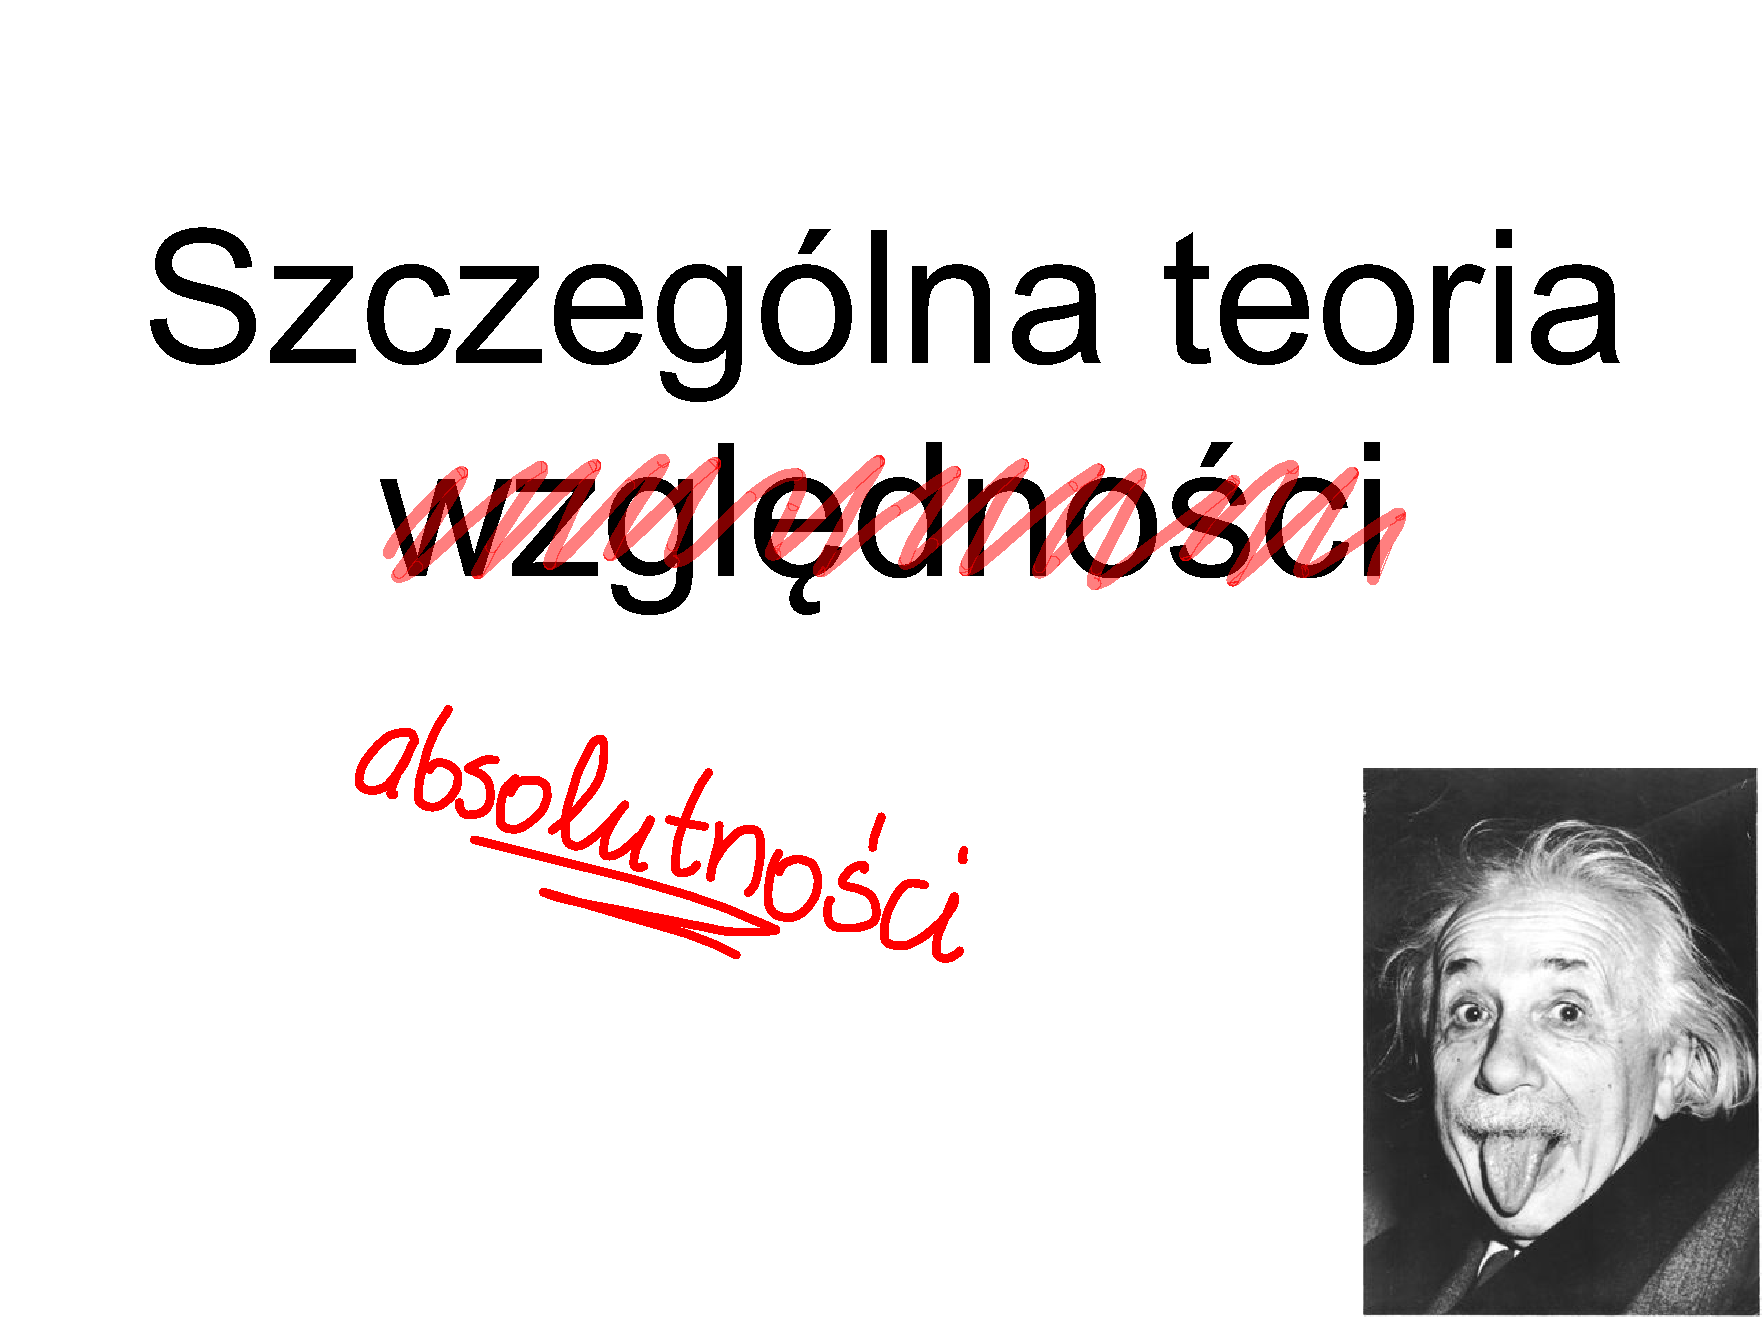
\includegraphics[width=1\linewidth]{pages/STA-page0}
Cześć, w tym wykładzie omówię podstawy szczególnej teorii względności, która
zyskała wielką sławę i jeszcze więcej niezrozumienia.
Ponieważ obrazki są jak Rafaello i wyrażają więcej niż tysiąc słów, będę sporo
się nimi wspomagał.

Przejdziemy stopniowo od fizyki klasycznej jeszcze z czasów Galileusza do
równań Lorentza w czasoprzestrzeni Minkowskiego.
Opowiem dlaczego teoria względności jest nie taka względna jak by chciała
oraz policzymy ile czasu gotuje się jajko na statku kosmicznym.
Rozwiążemy też odwieczne pytanie czy tyczka zmieści się w stodole oraz jak
szybko porusza się fala meksykańska.
Na koniec wyjaśnię dlaczego $E$ nie równa się $mc^2$.

Niestety, większość zagadnień jest omówiona dość powierzchownie, bo inaczej
cały wykład zająłby kilkaset stron i wiele miesięcy pisania.
Zachęcam cię zatem do głębszego przeanalizowania informacji zawartych na każdej stronie
i zadawania dodatkowych pytań i udzielania na nich odpowiedzi.
\newpage

\section{Wszystko było dobrze, dopóki nie przestało być}
\noindent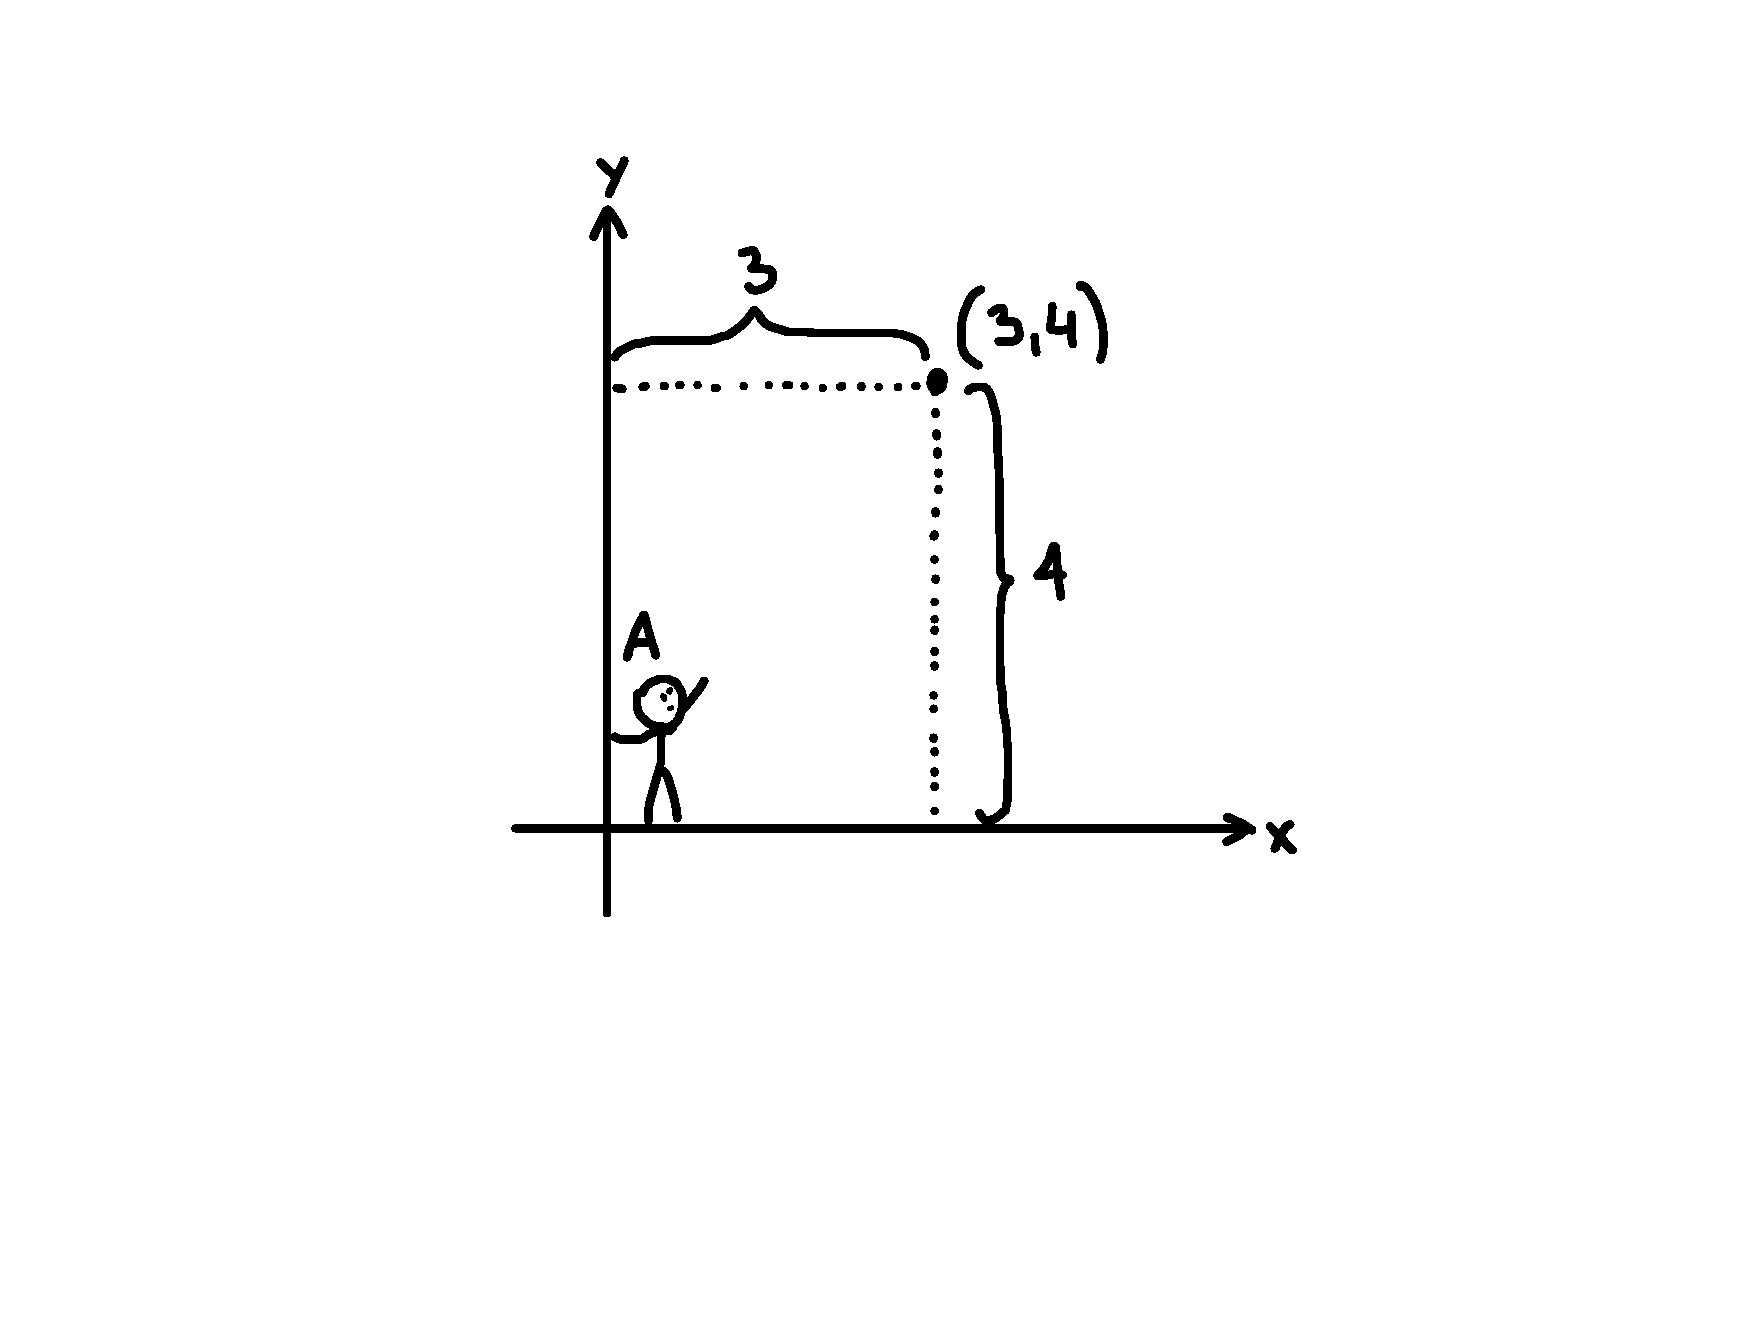
\includegraphics[width=1\linewidth]{pages/STA-page1}
Poznajcie Alfreda. Alfred żyje w dwu-wymiarowym układzie współrzędnych,
w którym nie dzieje się zbyt wiele. W zasadzie nie dzieje się zupełnie nic, bo
w tym układzie nie ma czasu. Jest tylko przestrzeń i nieruchomy punkt
zawieszony w pustce, które Alfred lubi obserwować. Ponieważ nie ma wokół żadnego
punktu odniesienia, Alfred wybrał samego siebie jako centrum układu.
Przecież każdy układ jest równie dobry, prawda?

My mieszkający na Ziemi intuicyjnie wybieramy powierzchnię Ziemi jako
układ odniesienia, według którego mierzymy położenie i prędkość.
Nie jest to jedyny słuszny wybór, bo każdy układ inercjalny jest równie prawidłowy.
Niektóre są jednak dla nas bardziej użyteczne od innych.
Sytuacja drastycznie zmienia się w przestrzeni kosmicznej, gdzie
takiego punktu zaczepienia nie ma.
\newpage

\noindent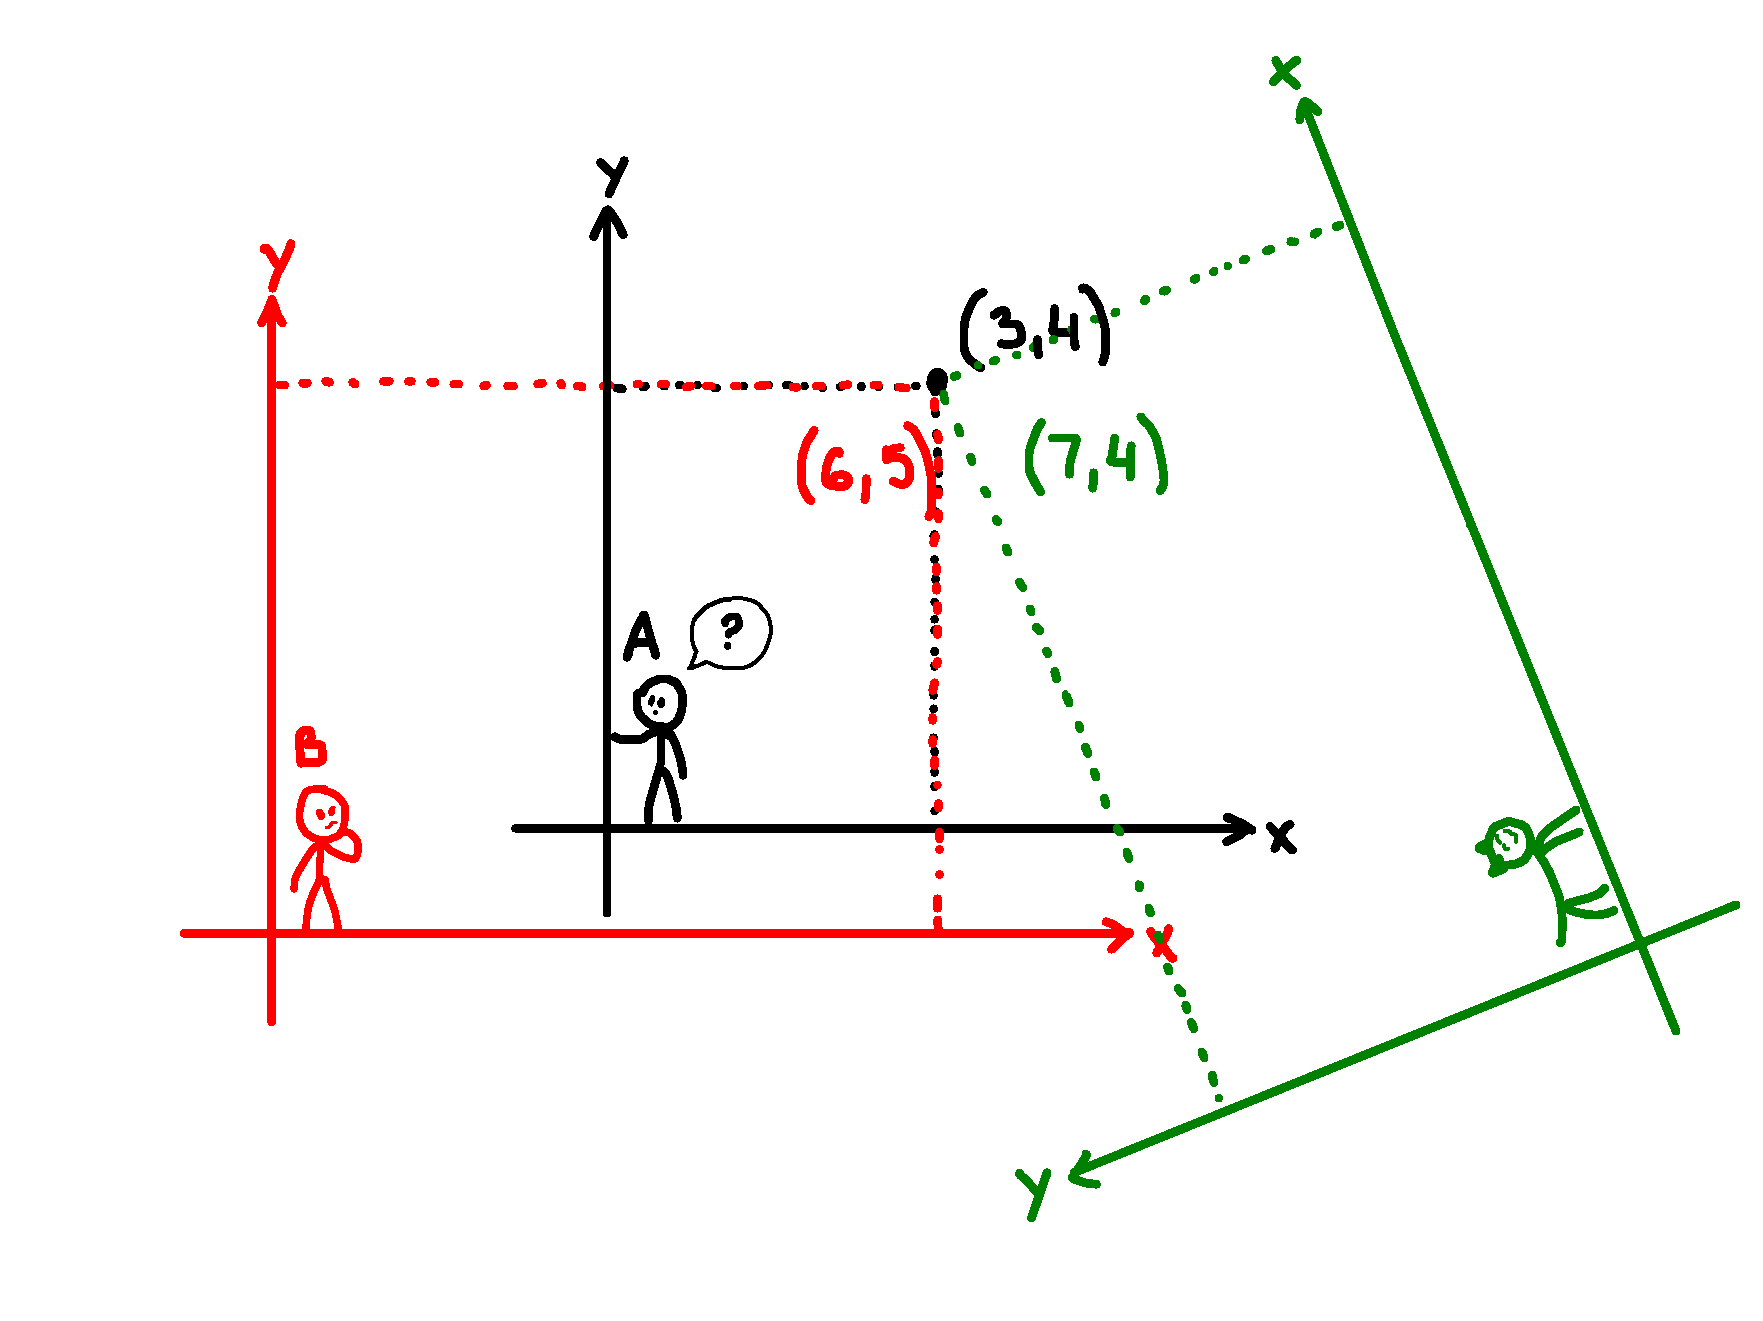
\includegraphics[width=1\linewidth]{pages/STA-page2}
Problemy zaczęły się (a raczej były zawsze z powodu nieistnienia czasu),
gdy Alfred chciał wskazać punkt Beacie i jej kotu.
Okazuje się, że położenie mierzone przez Alfreda było niezgodne z obserwacjami innych.
Oczywiście różne obserwacje wynikały z odmiennego położenia
lub orientacji obserwatorów względem Alfreda.
By zrozumieć jak inni widzą przestrzeń, Alfred musi dokonać transformacji
współrzędnych\footnotemark:
\[
  \begin{eqsystem}
    \mathcolor{BrickRed}{x'} = x - x_{BA} \\
    \mathcolor{BrickRed}{y'} = y - y_{BA},
  \end{eqsystem}
\]
gdzie $(x, y)$ i $(\mathcolor{BrickRed}{x'}, \mathcolor{BrickRed}{y'})$ to położenie
punktu zanotowane kolejno przez Alfreda i Beatę, a $(x_{BA}, y_{BA})$ to położenie
Beaty z punktu widzenia Alfreda.
\footnotetext{Pełna transformacja uwzględniająca obrót jest opisana w dodatkach}
\newpage

\noindent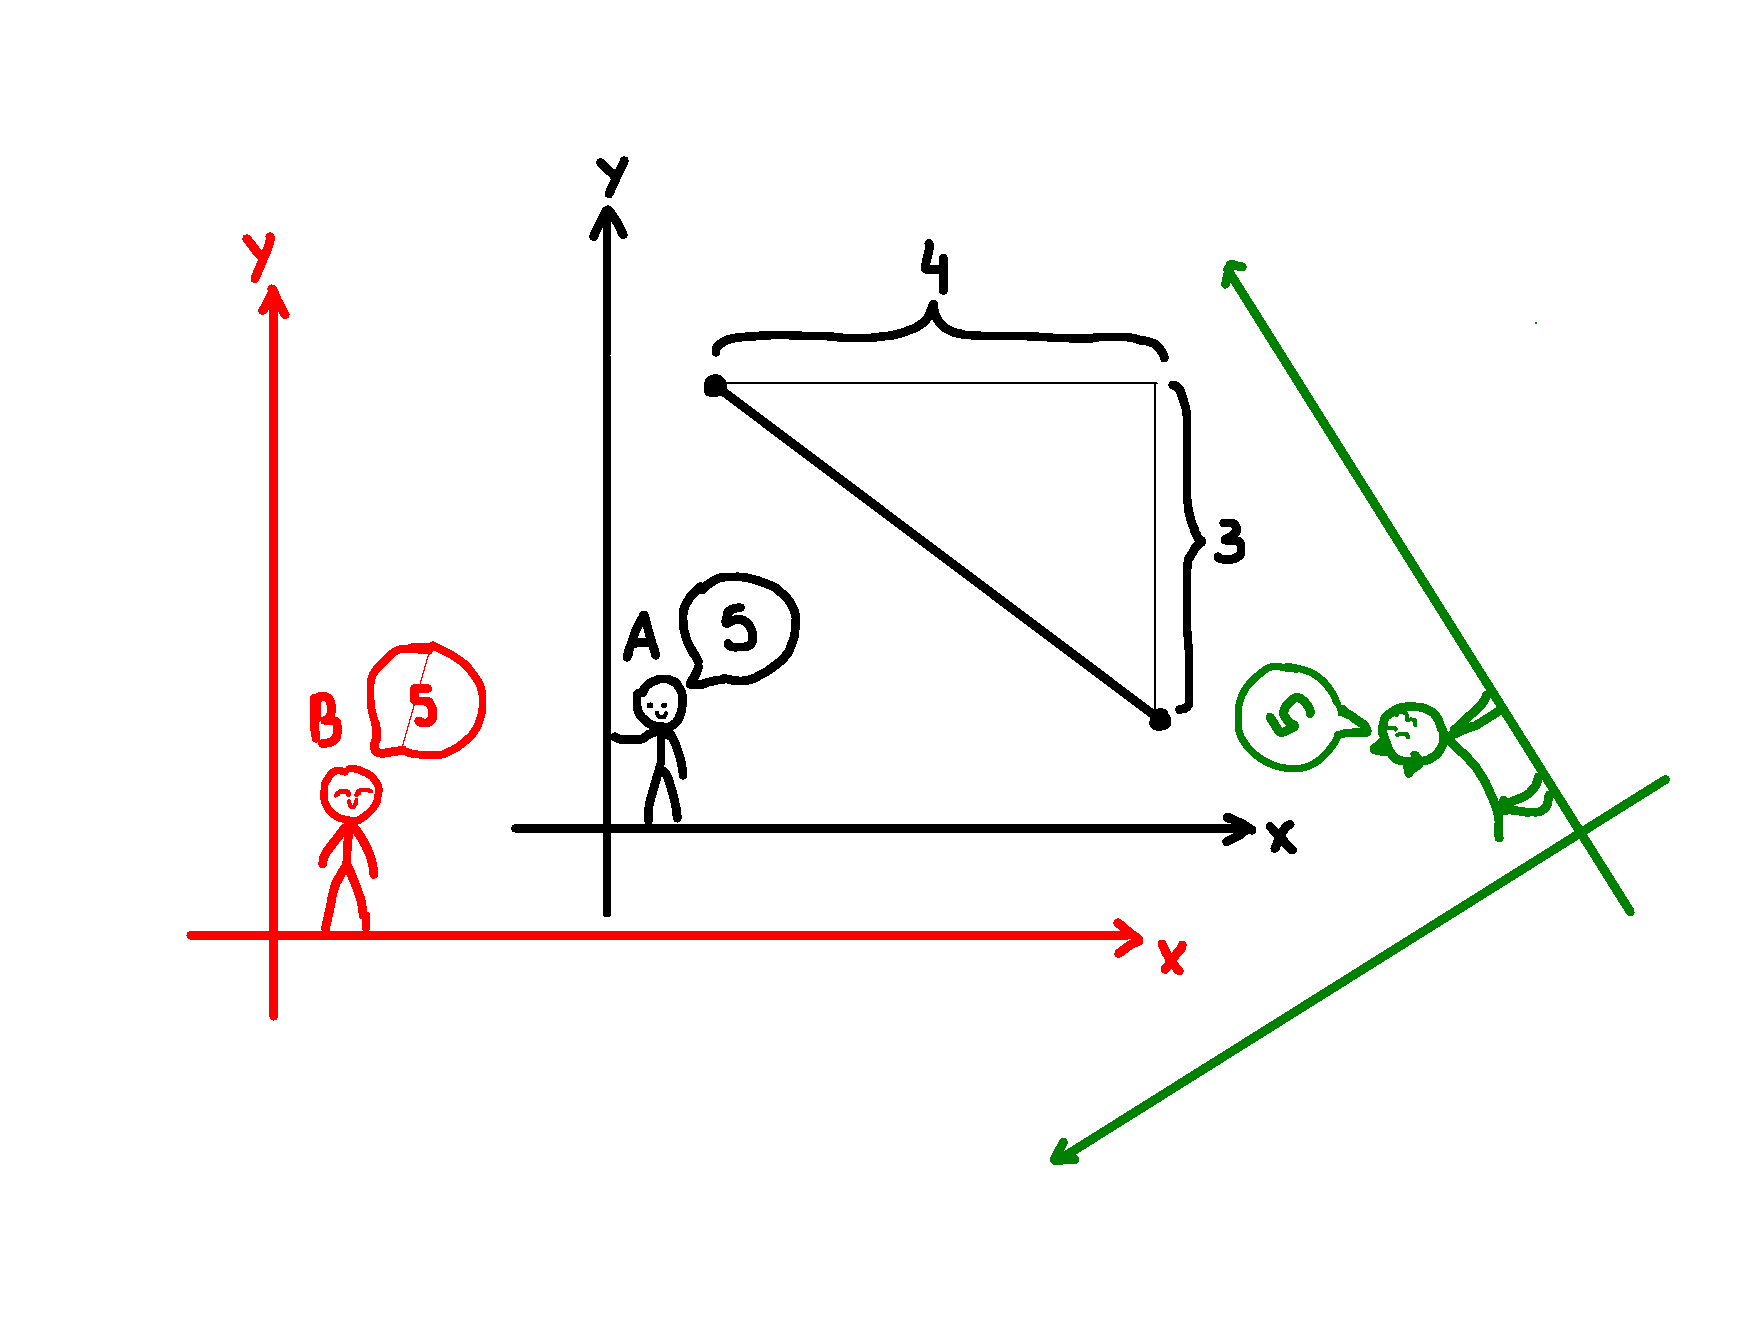
\includegraphics[width=1\linewidth]{pages/STA-page3}
Jeśli położenie jest względne to czy jest coś absolutnego? A może jesteśmy
skazani na życie w świecie gdzie wszystko jest zależne od wyboru obserwatora.

Jeśli dokładnie przeanalizujemy równanie transformacji współrzędnych,
okazuje się, że jest pewna wartość, która się nie zmienia pod wpływem
przesunięcia lub obrotu. Jest to $x^2 + y^2$ czyli inaczej
odległość między dwoma punktami.
Może nie jest to w pełni zadowalający rezultat, ale to przynajmniej
jedna wielkość co do której wszyscy są zgodni.
\newpage

\noindent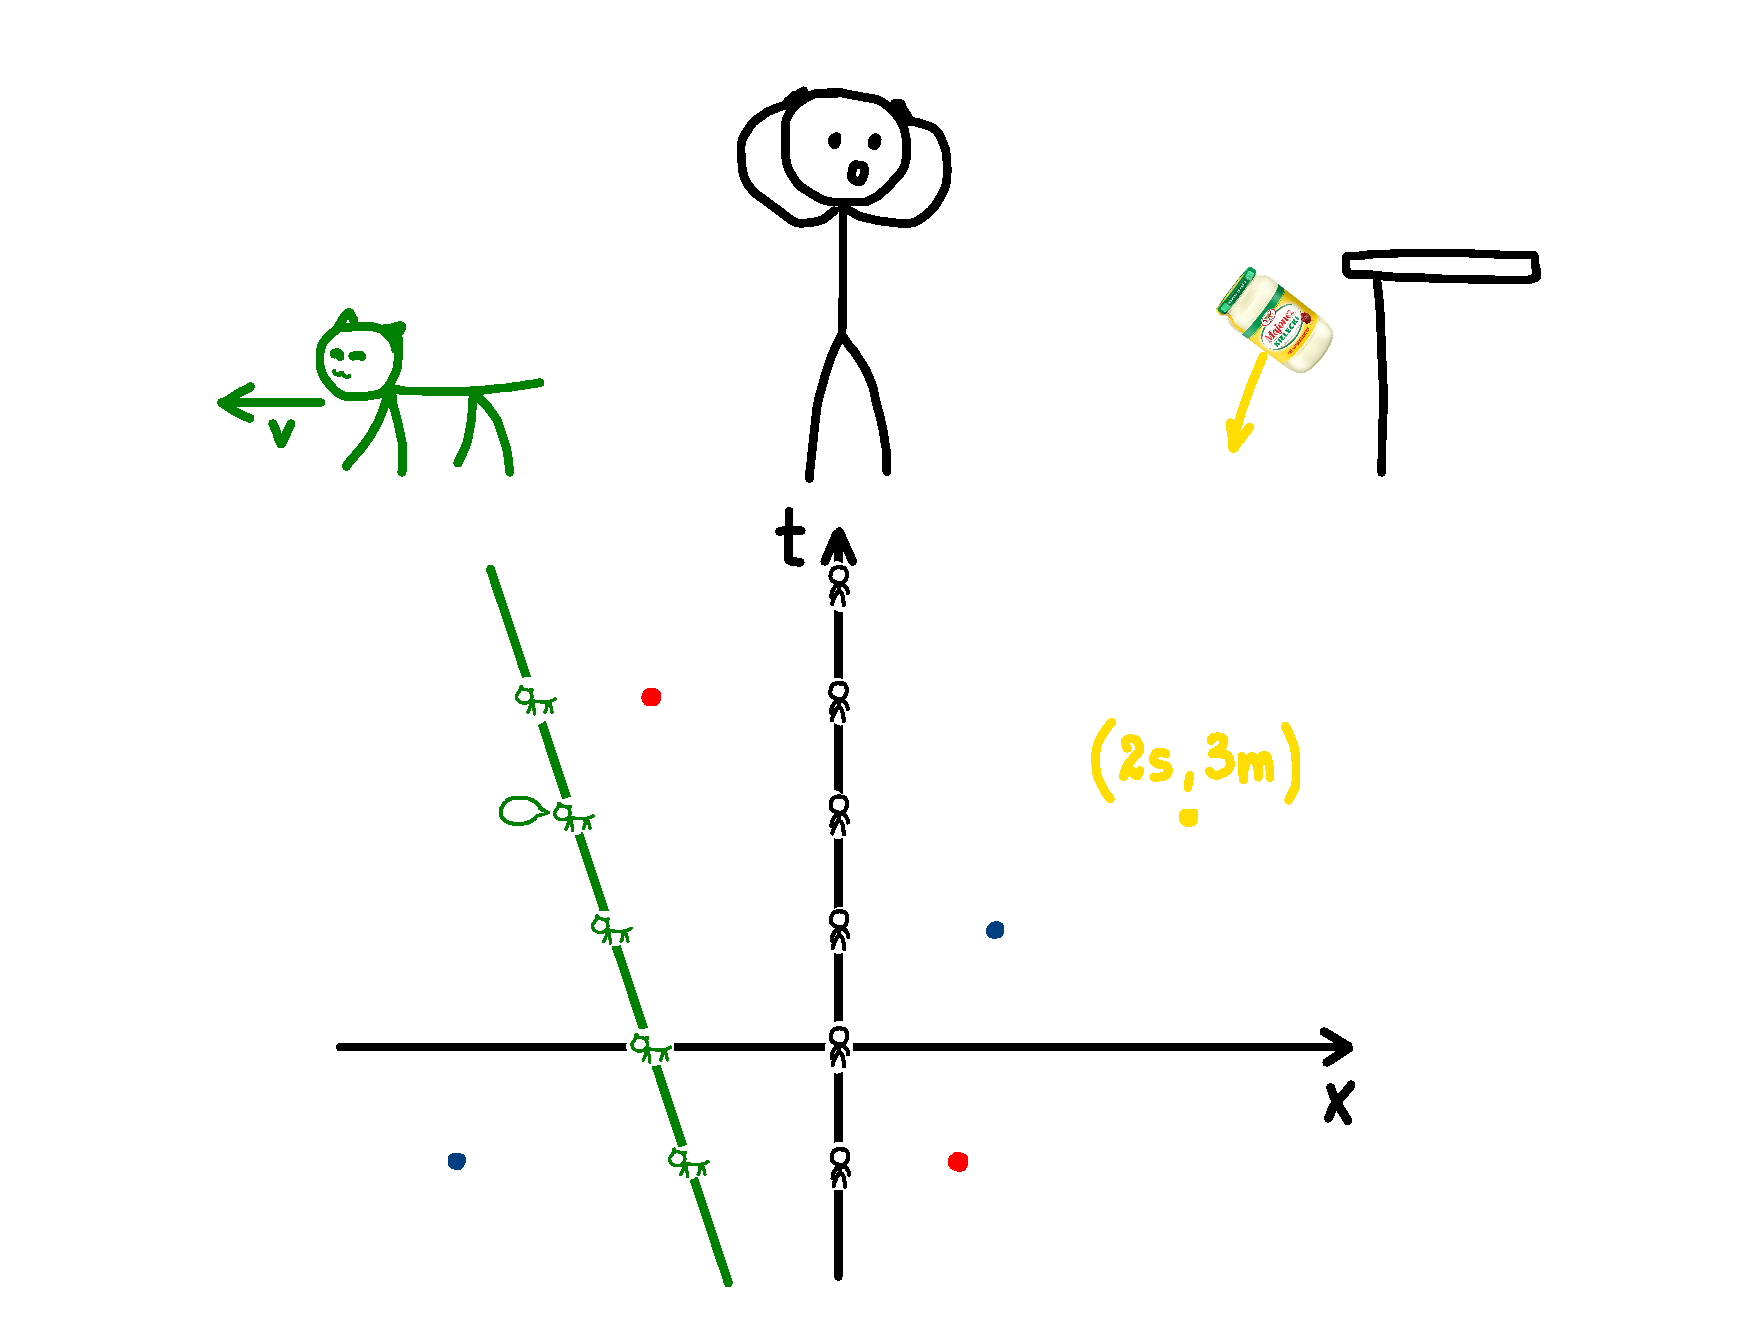
\includegraphics[width=1\linewidth]{pages/STA-page4}
Zróbmy teraz małą zmianę i dodajmy trochę akcji do świata Alfreda. Będzie
nam w tym celu potrzebny czas. Zamiast statycznych punktów będziemy od
teraz mówić o zdarzeniach, które mają jedną współrzędną czasową (kiedy się zdarzyły)
i jedną przestrzenną (gdzie się zdarzyły).

Zdarzenie jest niczym więcej jak punktem w czasoprzestrzeni.
Może oznaczać uderzenie słoika majonezu o podłogę lub sekwencję położeń kota.
Pamiętajmy, że położenie Alfreda w jego własnym
świecie zawsze będzie $x=0$ (no chyba, że Alfred wyjdzie z siebie i stanie obok,
ale to zdarza mu się bardzo rzadko).

Jeśli połączymy linią kolejne położenia w czasoprzestrzeni
otrzymamy ``linię świata''  danego obiektu, tor, którym porusza się w czasoprzestrzeni.
Linia świata Alfreda obserwowana przez niego samego będzie zawsze pokrywać się z osią czasu, bo
w swoim własnym układzie każdy jest nieruchomy.
Linie świata innych obiektów mogą być liniami prostymi równoległymi
do linii Alfreda, gdy ich położenie się nie zmienia, lub pochylone
pod kątem jeśli poruszają się ruchem jednostajnym.

Przypadek ruchu niejednostajnego będzie tu omawiany.
\newpage

\noindent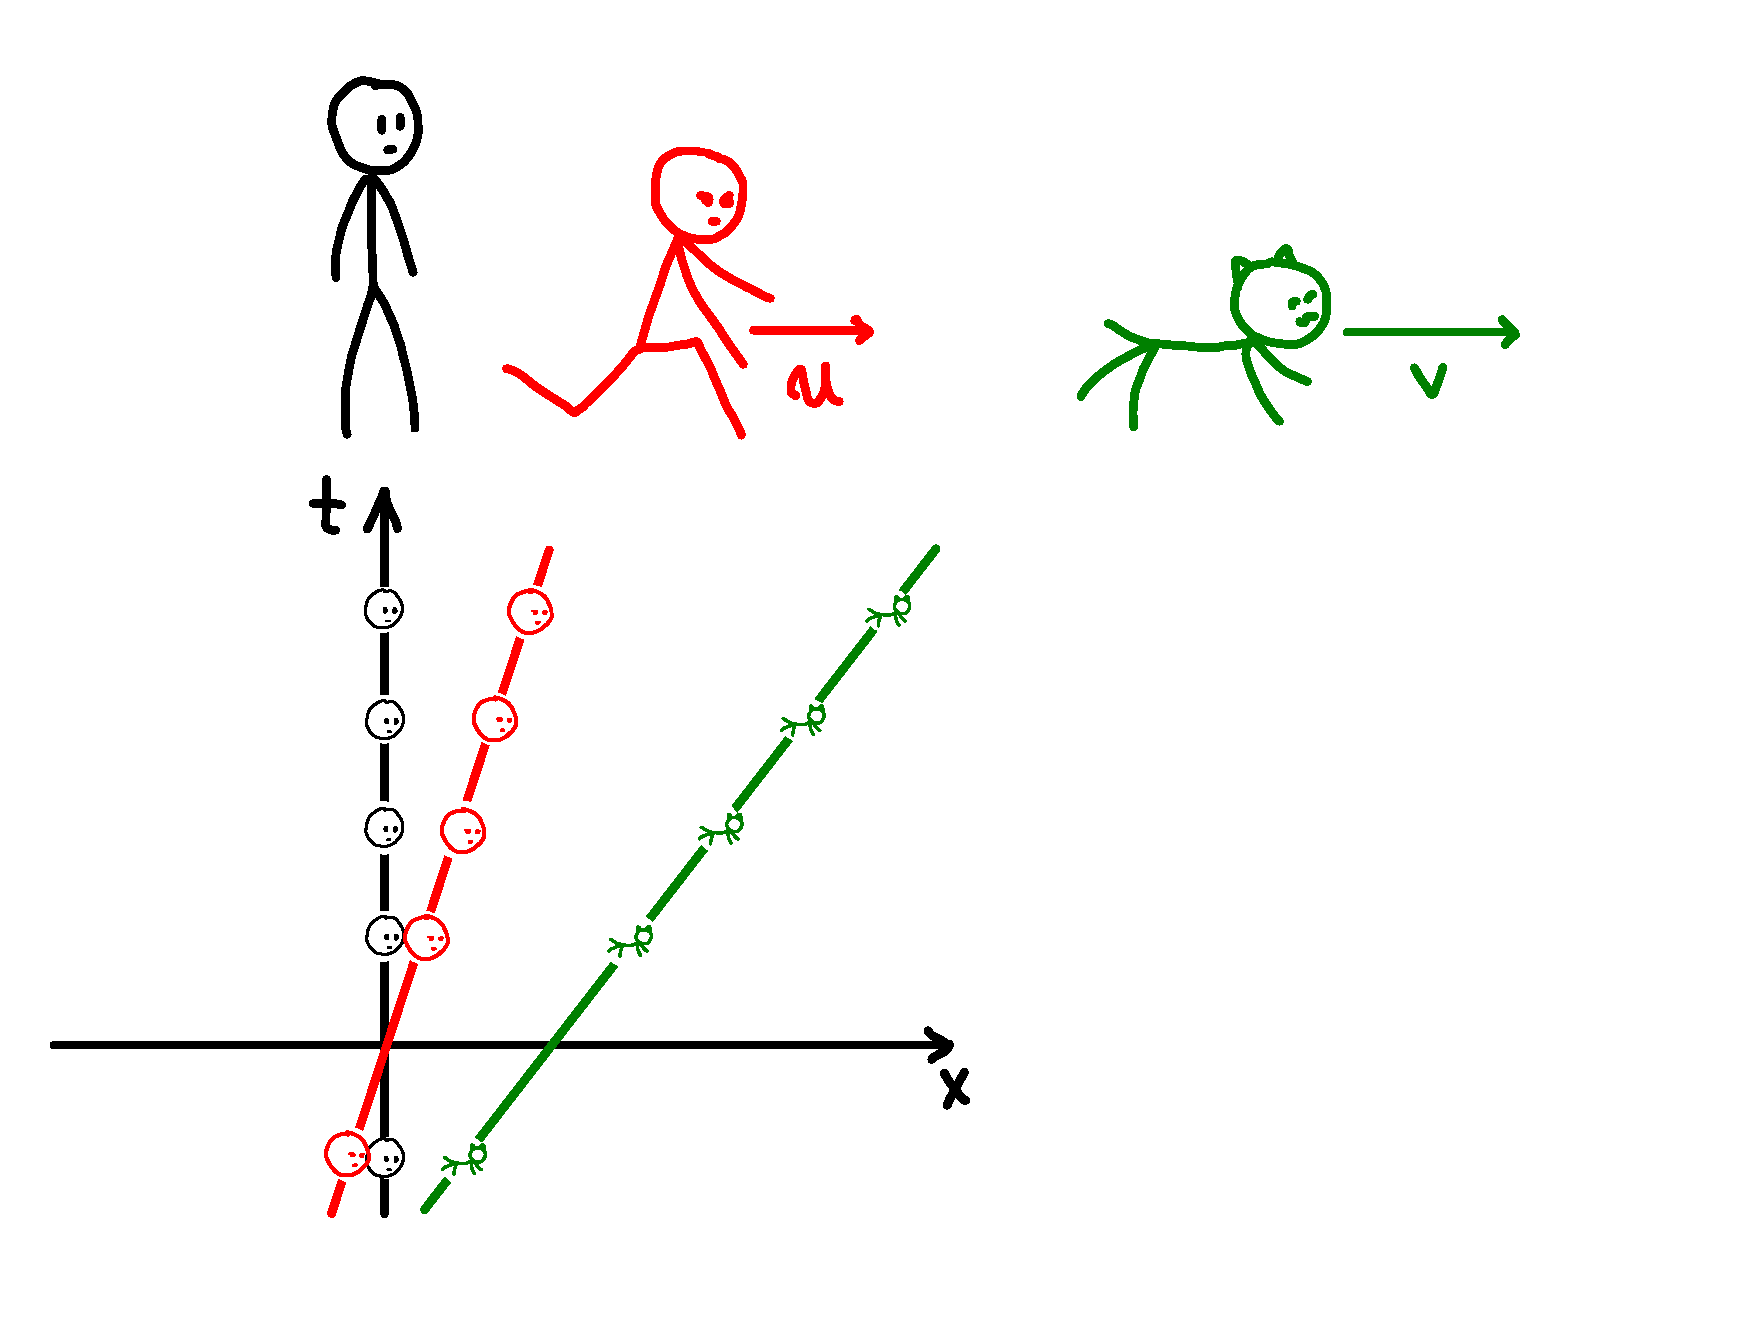
\includegraphics[width=1\linewidth]{pages/STA-page5}
Tak jak rozważaliśmy transformację położenia przy przesunięciu
się w inne miejsce w przestrzeni, podobnie możemy transformować
współrzędne czasoprzestrzenne gdy zmieniamy położenie lub prędkość.

Jeśli będziemy obserwować położenie kota względem Alfreda i Beaty,
nie tylko położenie kota będzie inne, ale dojdziemy też do wniosku,
że kot od Beaty oddala się wolniej.
Nie jest w tym nic dziwnego skoro Beata go goni.

Albert może opisać położenie Beaty i kota prostymi wzorami:
\[ \mathcolor{Blue}{x_B} = u\mathcolor{Blue}{t}, \]
\[ \mathcolor{Blue}{x_K} = {x_K}_0 + v\mathcolor{Blue}{t}. \]
Zatem położenie kota z punktu widzenia Beaty będzie wynosić:
\[
  \mathcolor{BrickRed}{x_K'}
  = \mathcolor{Blue}{x_K} - \mathcolor{Blue}{x_B}
  = {\color{Blue}x_K} - u\mathcolor{Blue}{t}
    = {x_K}_0 + (v-u)\mathcolor{Blue}{t}.
\]
\newpage

\noindent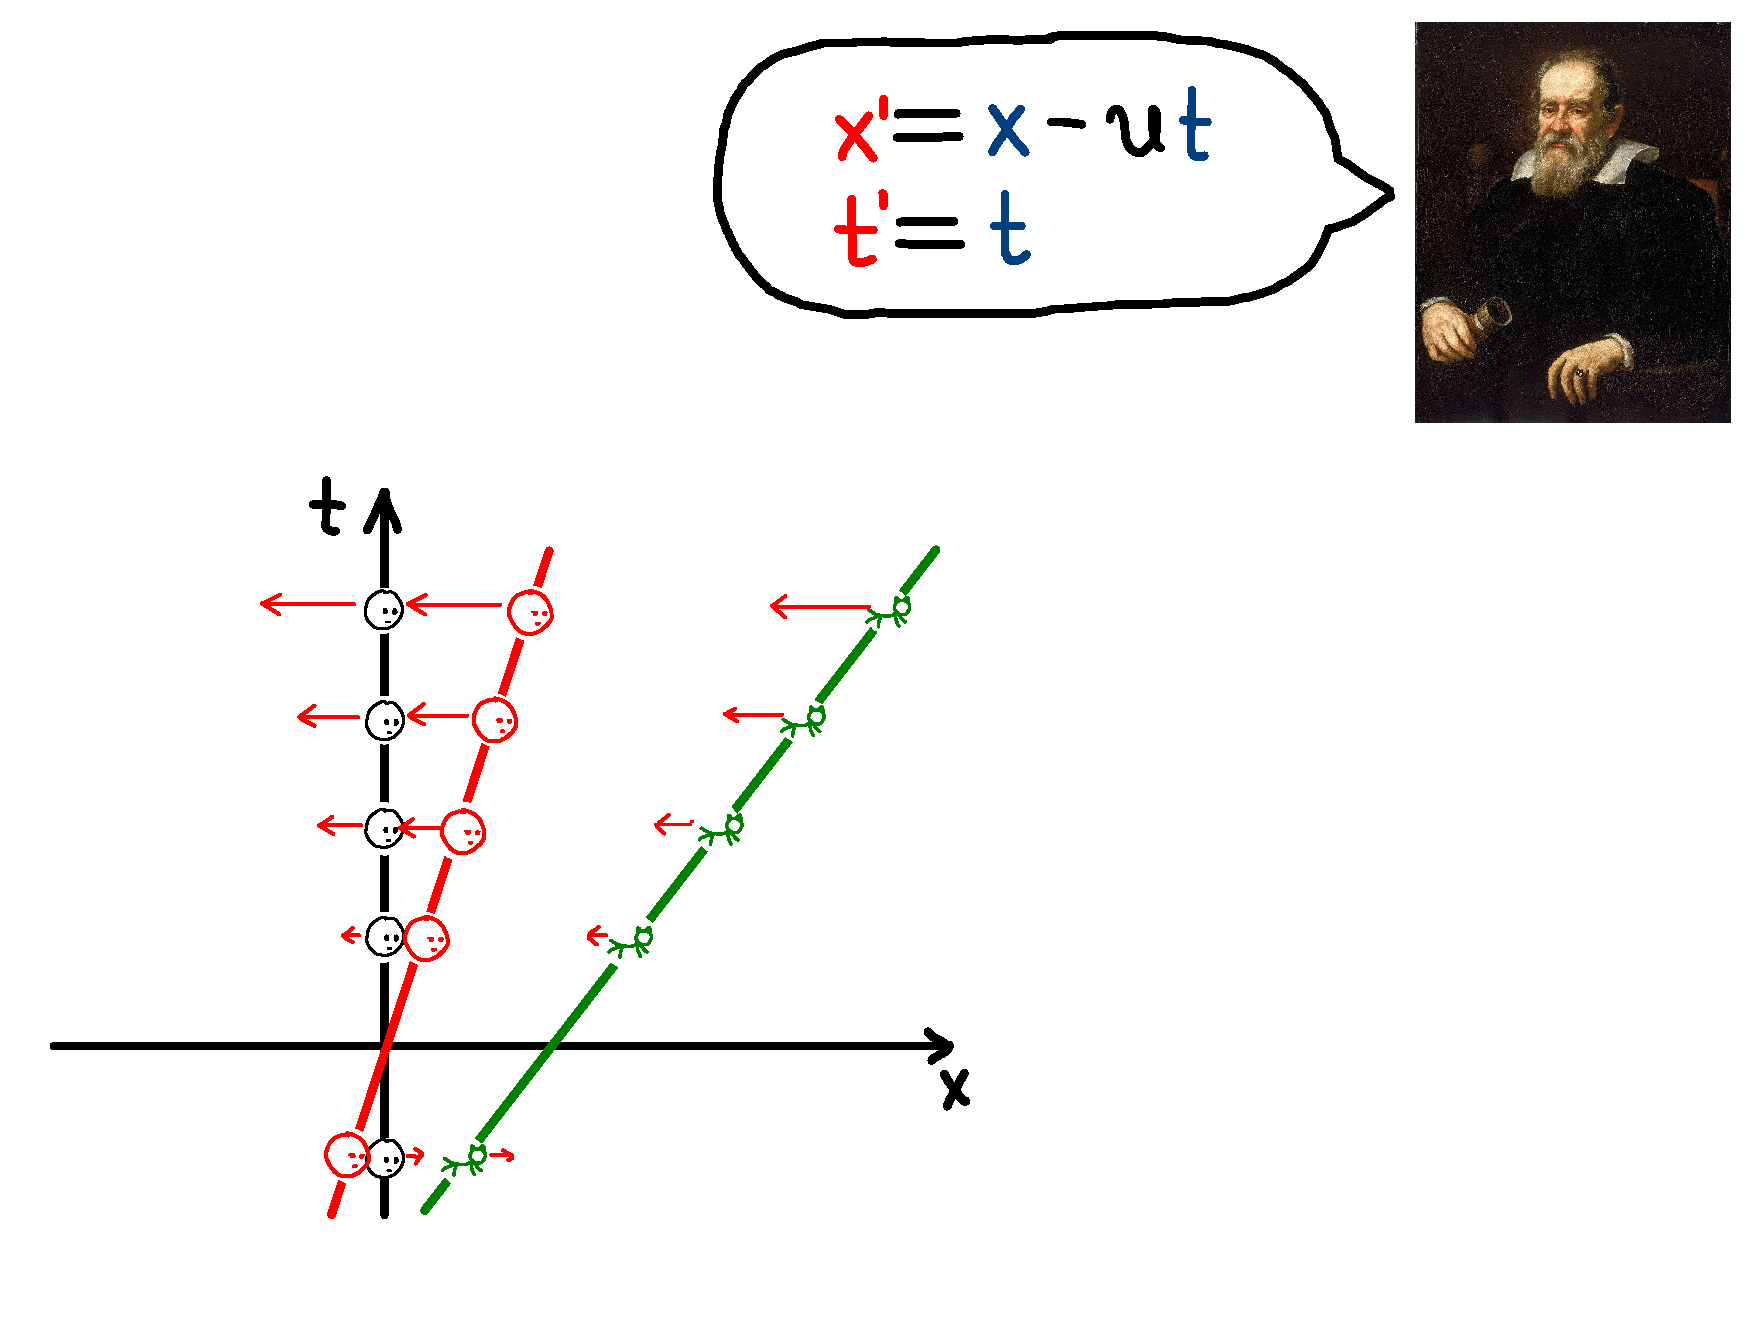
\includegraphics[width=1\linewidth]{pages/STA-page6}
Takie przekształcenie współrzędnych czasoprzestrzennych nie jest żadną
nowością w świecie fizyki. Były opisane jeszcze przez Galileusza na przełomie
XVI i XVII wieku. Transformacja Galileusza mówi nam, że przy zmianie układu
odniesienia obliczając położenie zdarzenia musimy też uwzględnić jego czas.
Nowe współrzędne będą wynosić:
\[
  \begin{eqsystem}
    \mathcolor{BrickRed}{x'} = \mathcolor{Blue}{x} - u\mathcolor{Blue}{t} \\
    \mathcolor{BrickRed}{t'} = \mathcolor{Blue}{t}
  \end{eqsystem}
\]

Graficznie jest to przesunięcie wszystkich punktów równolegle do osi $x$
(prostopadle do osi $t$) tak aby teraz to linia świata Beaty pokrywała
się z osią czasu.
\newpage

\noindent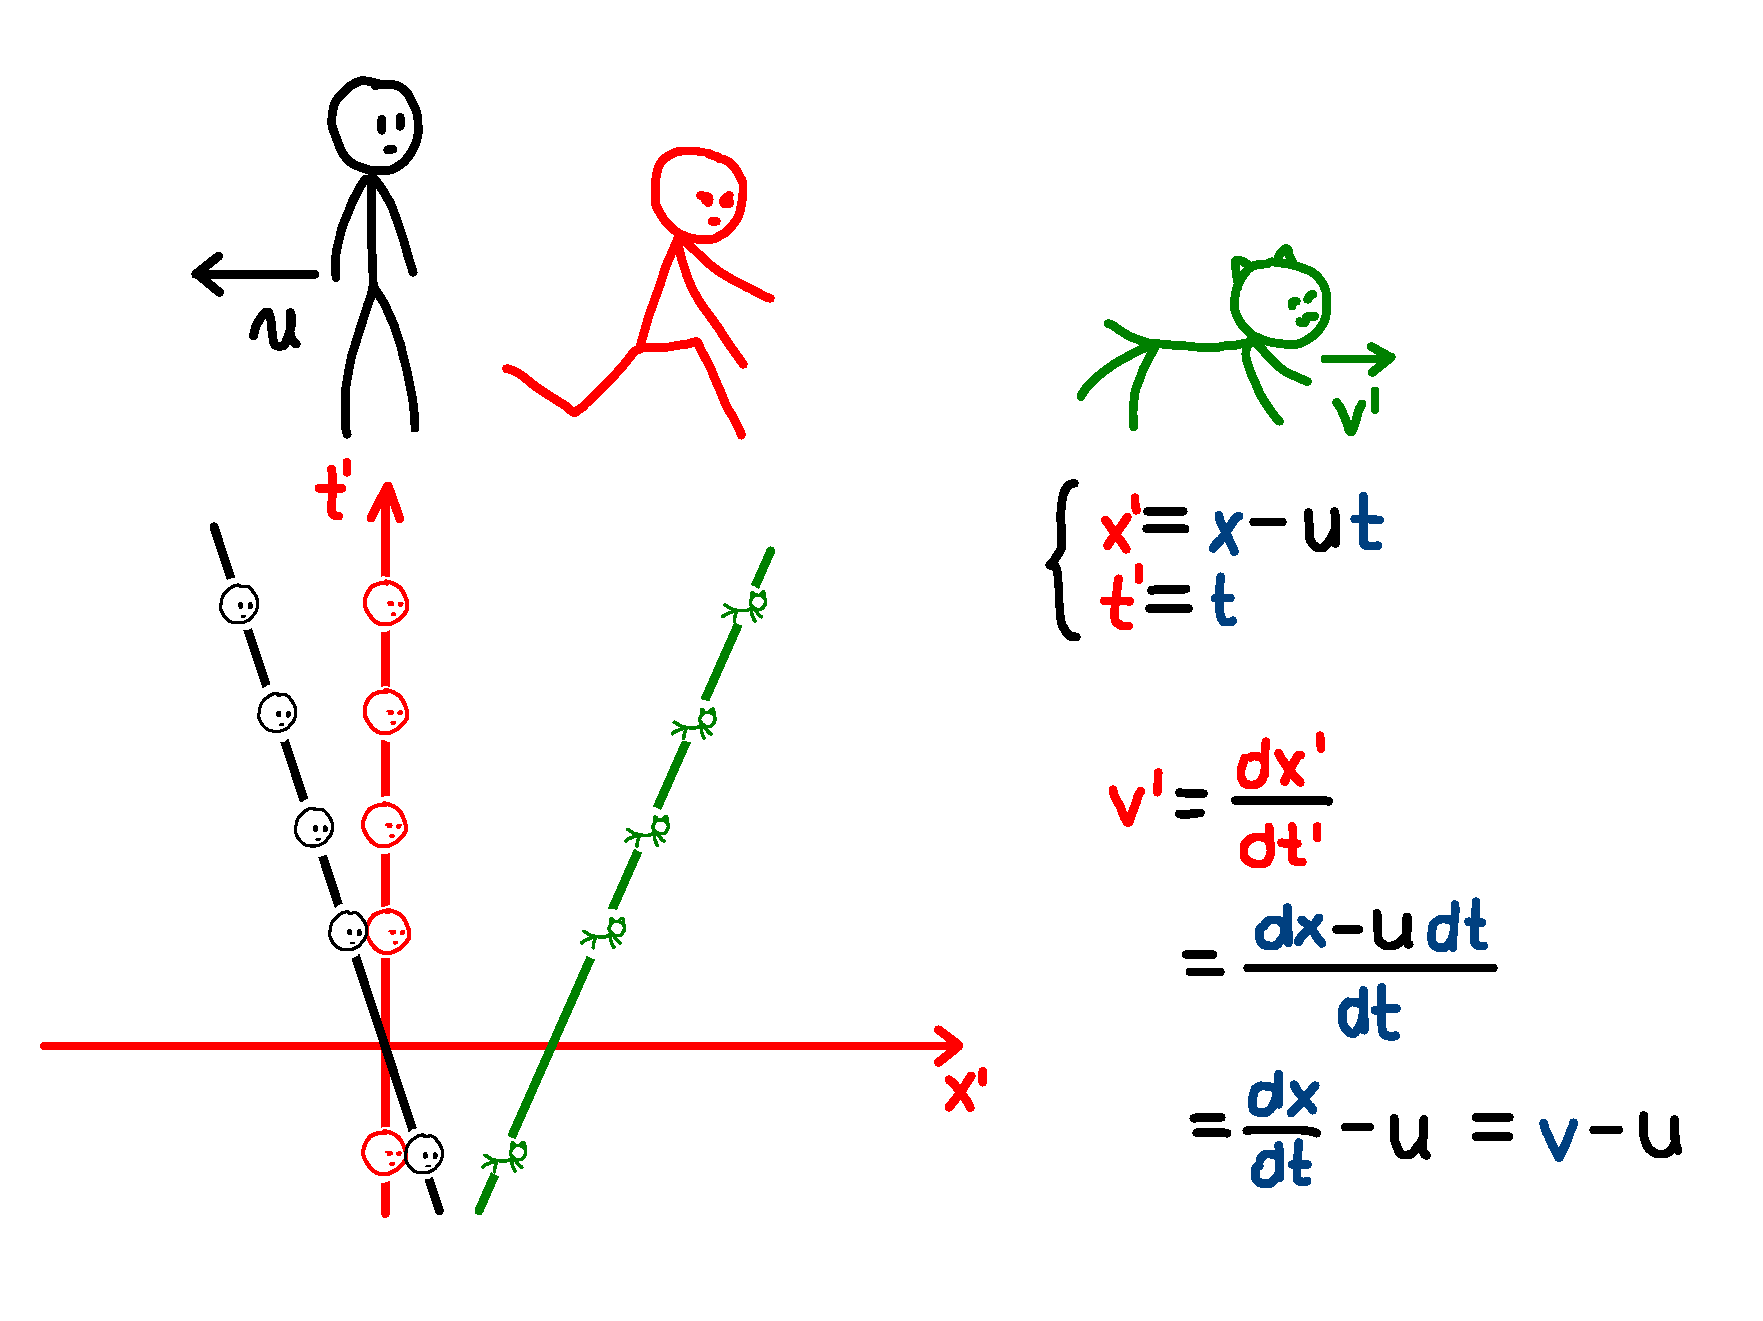
\includegraphics[width=1\linewidth]{pages/STA-page7}
Po transformacji możemy obserwować świat oczami Beaty, w którym Alfred
dostaje w tyle i oddala się z szybkością $u$ a kot nadal pozostaje
niedościgniony, ale teraz trochę mniej.

Zanim przejdziemy dalej możemy zweryfikować regułę dodawania prędkości.
Zaczynając od równań transformacji możemy zamienić współrzędne na
malutkie przyrosty $\diff x$ i $\diff t$ a następnie wstawić je do wyrażenia na prędkość.
\begin{gather*}
  \begin{eqsystem}
    \mathcolor{BrickRed}{x'} = \mathcolor{Blue}{x}- u\mathcolor{Blue}{t} \\
    \mathcolor{BrickRed}{t'} = \mathcolor{Blue}{t}
  \end{eqsystem} \\
  \begin{eqsystem}
    \mathcolor{BrickRed}{\diff x'} = \mathcolor{Blue}{\diff x}- u\mathcolor{Blue}{\diff t} \\
    \mathcolor{BrickRed}{\diff t'} = \mathcolor{Blue}{\diff t}
  \end{eqsystem}
\end{gather*}
\[
  \mathcolor{BrickRed}{v'}
  = \mathcolor{BrickRed}{\derivative[x']{t'}}
  = \frac{\mathcolor{Blue}{\diff x} - u \mathcolor{Blue}{\diff t}}{\mathcolor{Blue}{\diff t}}
  = {\color{Blue}\derivative[x]{t}} - u
    = {\color{Blue}{v}} - u
\]
Jak widać matematyka dała nam ten sam wynik, który znaliśmy już wcześniej.
\newpage

\noindent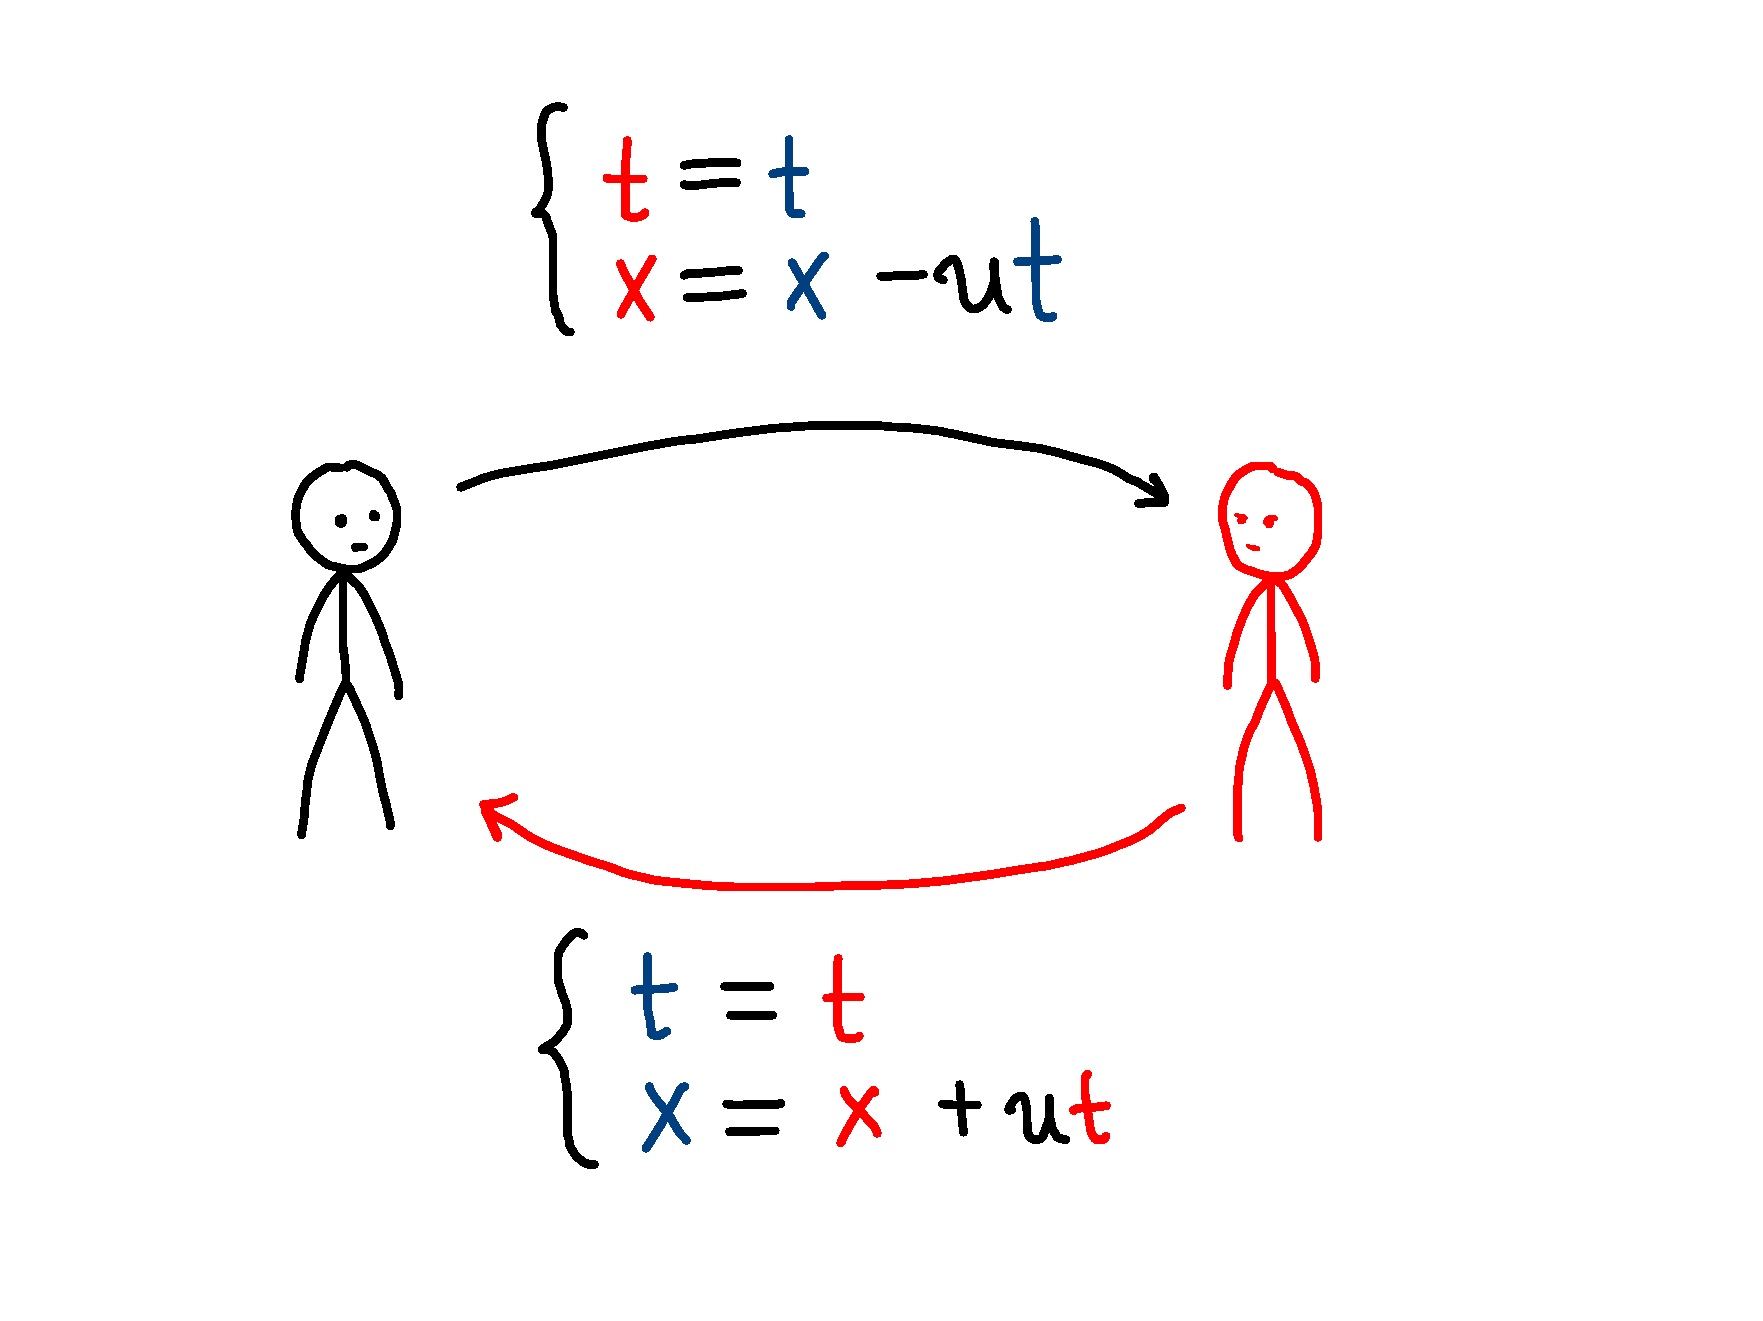
\includegraphics[width=1\linewidth]{pages/STA-page8}
Transformacja Galileusza ma jeszcze jedną bardzo ważną właściwość,
jest symetryczna względem kierunków. Ani układ Alfreda ani Beaty nie jest uprzywilejowany
i przejście z jednego do drugiego odbywa się w identyczny sposób.
W końcu z punktu widzenia Alfreda Beata porusza się z prędkością $u$,
ale z jej punktu widzenia to Alfred się porusza z tą samą prędkością
tylko w przeciwnym kierunku.
\newpage

\subsection*{Pytania}
\begin{itemize}
  \item Jakie jest położenie Alfreda względem Beaty jeśli Beata według Alfreda
        znajduje się w punkcie $(-5, 3)$
  \item Jakie położenie kota zaobserwuje Beata, jeśli Alfred odnotował
        współrzędne kota $(8, 4)$ i współrzędne Beaty $(3, 6)$?
  \item Jakie jest położenie Alfreda względem Beaty jeśli
        odnotowane przez nich położenie kota to kolejno $(3, 4)$ oraz $(6,5)$?
  \item Jakie przekształcą się współrzędne gdy obrócimy układ o \SI{90}{\degree}
        przeciwnie do ruchu wskazówek zegara?
  \item Przy ulicy stoją dwie sygnalizacje świetlne oddalone od siebie o \SI{500}{\metre}.
        Drugie światło zmienia się na zielone dokładnie \SI{30}{s} po pierwszym.
        Z jaką prędkością należy jechać aby obie zmiany świateł zaszły w tym samym miejscu
        (mierzonym przed kierowcę samochodu)?
\end{itemize}
\newpage

\section{Problem elektromagnetyczny}

\noindent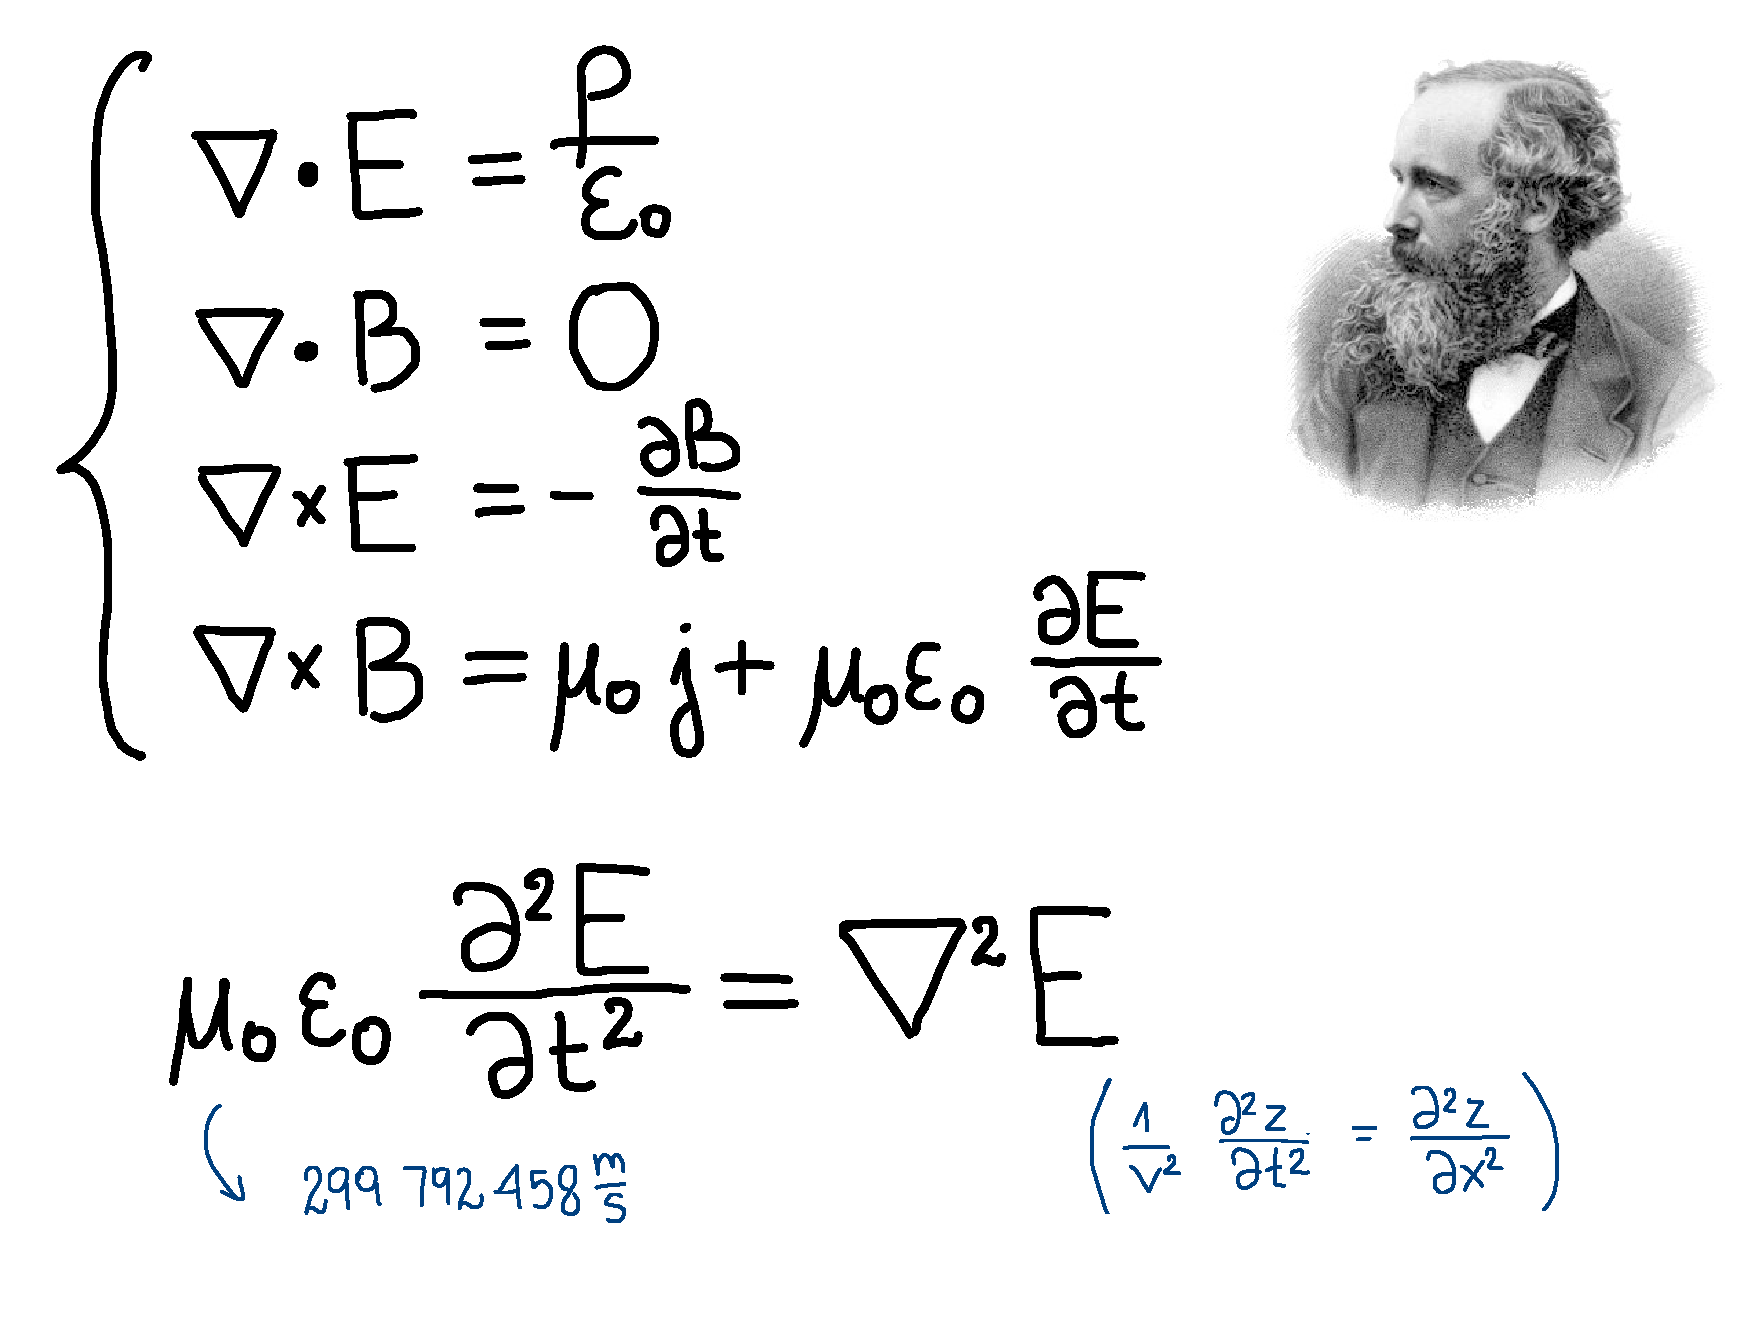
\includegraphics[width=1\linewidth]{pages/STA-page9}
Dotychczasowa kinematyka opisywała ruch bardzo starannie, dopóki James Clerk Maxwell
nie namieszał swoją teorią elektromagnetyzmu. Sformułował on cztery
równania opisujące zmiany pola elektrycznego i magnetycznego w pobliżu
stojących lub płynących ładunków elektrycznych oraz ich wzajemny wpływ na siebie.
\begin{align*}
  \nabla \cdot \vec E  & = \frac{\rho}{\varepsilon_0}                                             &
  \nabla \times \vec E & = - \frac{\partial \vec B}{\partial t}                                     \\
  \nabla \cdot \vec B  & = 0                                                                      &
  \nabla \times \vec B & = \mu_0 \vec j + \mu_0 \varepsilon_0 \frac{\partial \vec E}{\partial t},
\end{align*}
gdzie $\rho$ to ładunek elektryczny przypadającym na jednostkę objętości a $\vec j$ to natężenie
prądu na jednostkę powierzchni przez którą przepływa.
Operator $\nabla$ (nabla) jest pochodną pola wektorowego po kierunkach $x, y, z$.
Bez wchodzenia w matematyczne szczegóły możemy zaobserwować, że zmiany pola elektromagnetycznego
mogą występować pod całkowitą nieobecność ładunków elektrycznych, gdy $\rho = 0$ i $\vec j = 0$.
Co więcej, podstawiając te równania do siebie nawzajem otrzymujemy równanie fali elektrycznej
\[\mu_0\varepsilon_0 \frac{\partial^2\vec E}{\partial t^2} = \nabla^2 \vec E.\]

Analogicznym równaniem dla wartości skalarnych np. fal na wodzie lub fal akustycznych
jest
\[
  \frac{1}{v^2} \frac{\partial^2 Z}{\partial t^2} = \frac{\partial^2 Z}{\partial x^2},
\]
gdzie $v$ to prędkość rozprzestrzeniania się fali. Przez analogię widać, że
nowo-odkryta fala elektromagnetyczna będzie rozchodzić się z szybkością
$\frac{1}{\sqrt{\mu_0\varepsilon_0}} = \SI{299792458}{\meter\per\second}$.

Fizycy szybko połączyli kropki, że wyznaczona szybkość rozchodzenia się fali
elektromagnetycznej jest taka sama co zmierzona eksperymentalnie prędkość
światła. Więc światło i elektromagnetyzm są ze sobą ściśle
związane lub nawet są tym samym.
Skoro jest fala, to musi istnieć też ośrodek, w którym się ta fala rozchodzi.
Bardzo skomplikowany ośrodek, który:
\begin{itemize}
  \item jest wektorowy, a nie skalarny,
  \item przenosi pole elektryczne i magnetyczne jednocześnie,
  \item wypełnia całą przestrzeń i kosmos wokół nas,
  \item przenika przez materię bez przeszkód,
  \item jest niezwykle sztywny, by móc utrzymywać tak ogromne prędkości fal.
\end{itemize}
Ośrodek nazwano \textit{eter} i od razu rozpoczęto jego intensywne badania.
\newpage

\noindent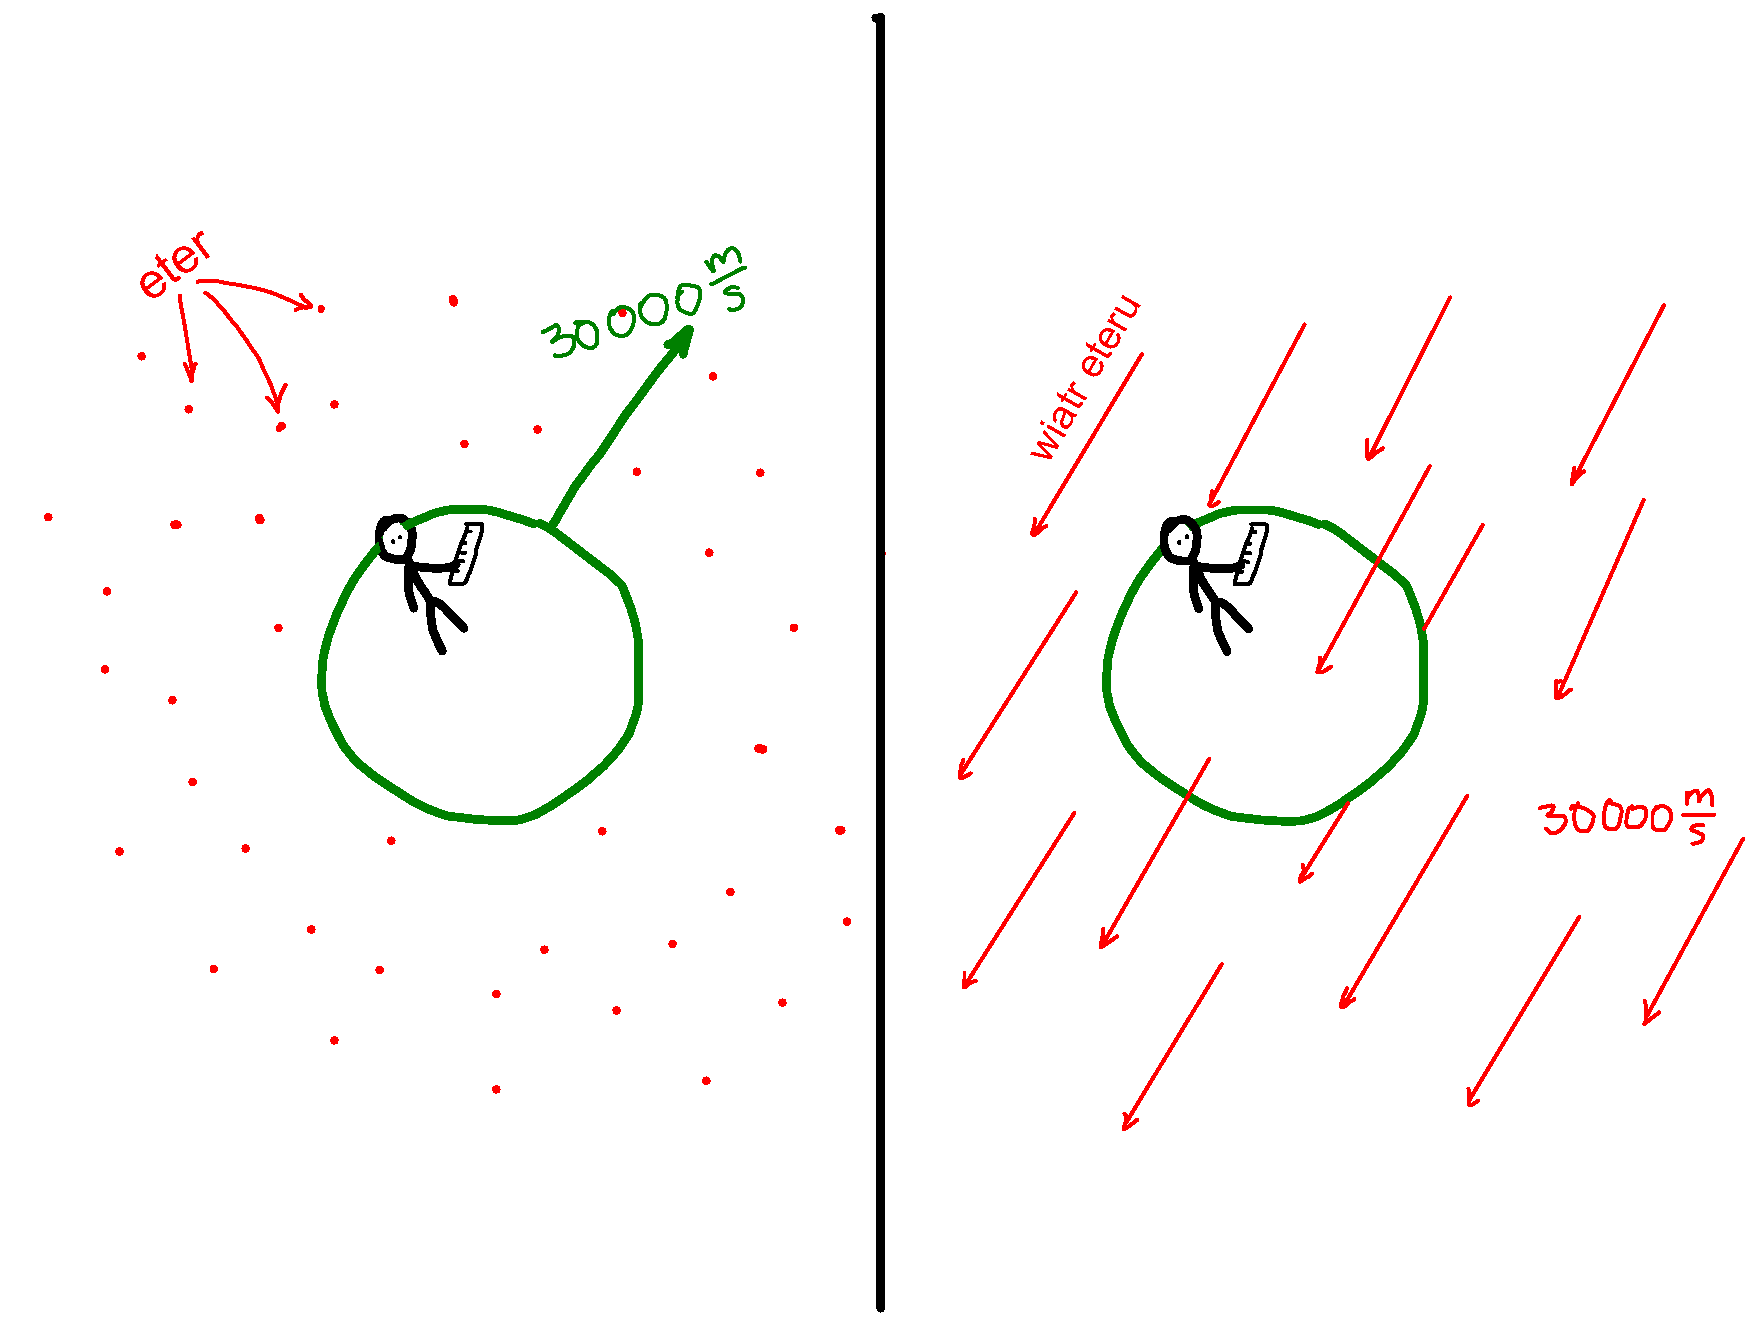
\includegraphics[width=1\linewidth]{pages/STA-page10}
Jednym z pomysłów na eksperyment badający eter była obserwacja \textit{wiatru eteru}.
Skoro cała przestrzeń kosmiczna jest nim wypełniona, a my siedząc na kamieniu
zwanym Ziemią przemierzamy przestrzeń z prędkością \SI{30}{\kilo\meter\per\second}
to stojąc na Ziemi powinniśmy odczuwać ``wiatr'' który będzie znosić światło
w jakimś kierunku. Ten kierunek zmieniałby się wraz z porą dnia i porami roku.

Pomysł był dobry jedynie w teorii. Żaden ówcześnie znany eksperyment nie był dość
dokładny by zmierzyć re odchylenia.
Najdokładniejsze pomiary prędkości światła miały margines błędu około
\SI{5}{\percent} zaś prędkość orbitalna Ziemi jest rzędu \SI{0.01}{\percent}
prędkości światła. Bezpośrednie pomiary były niemożliwe.
\newpage

\noindent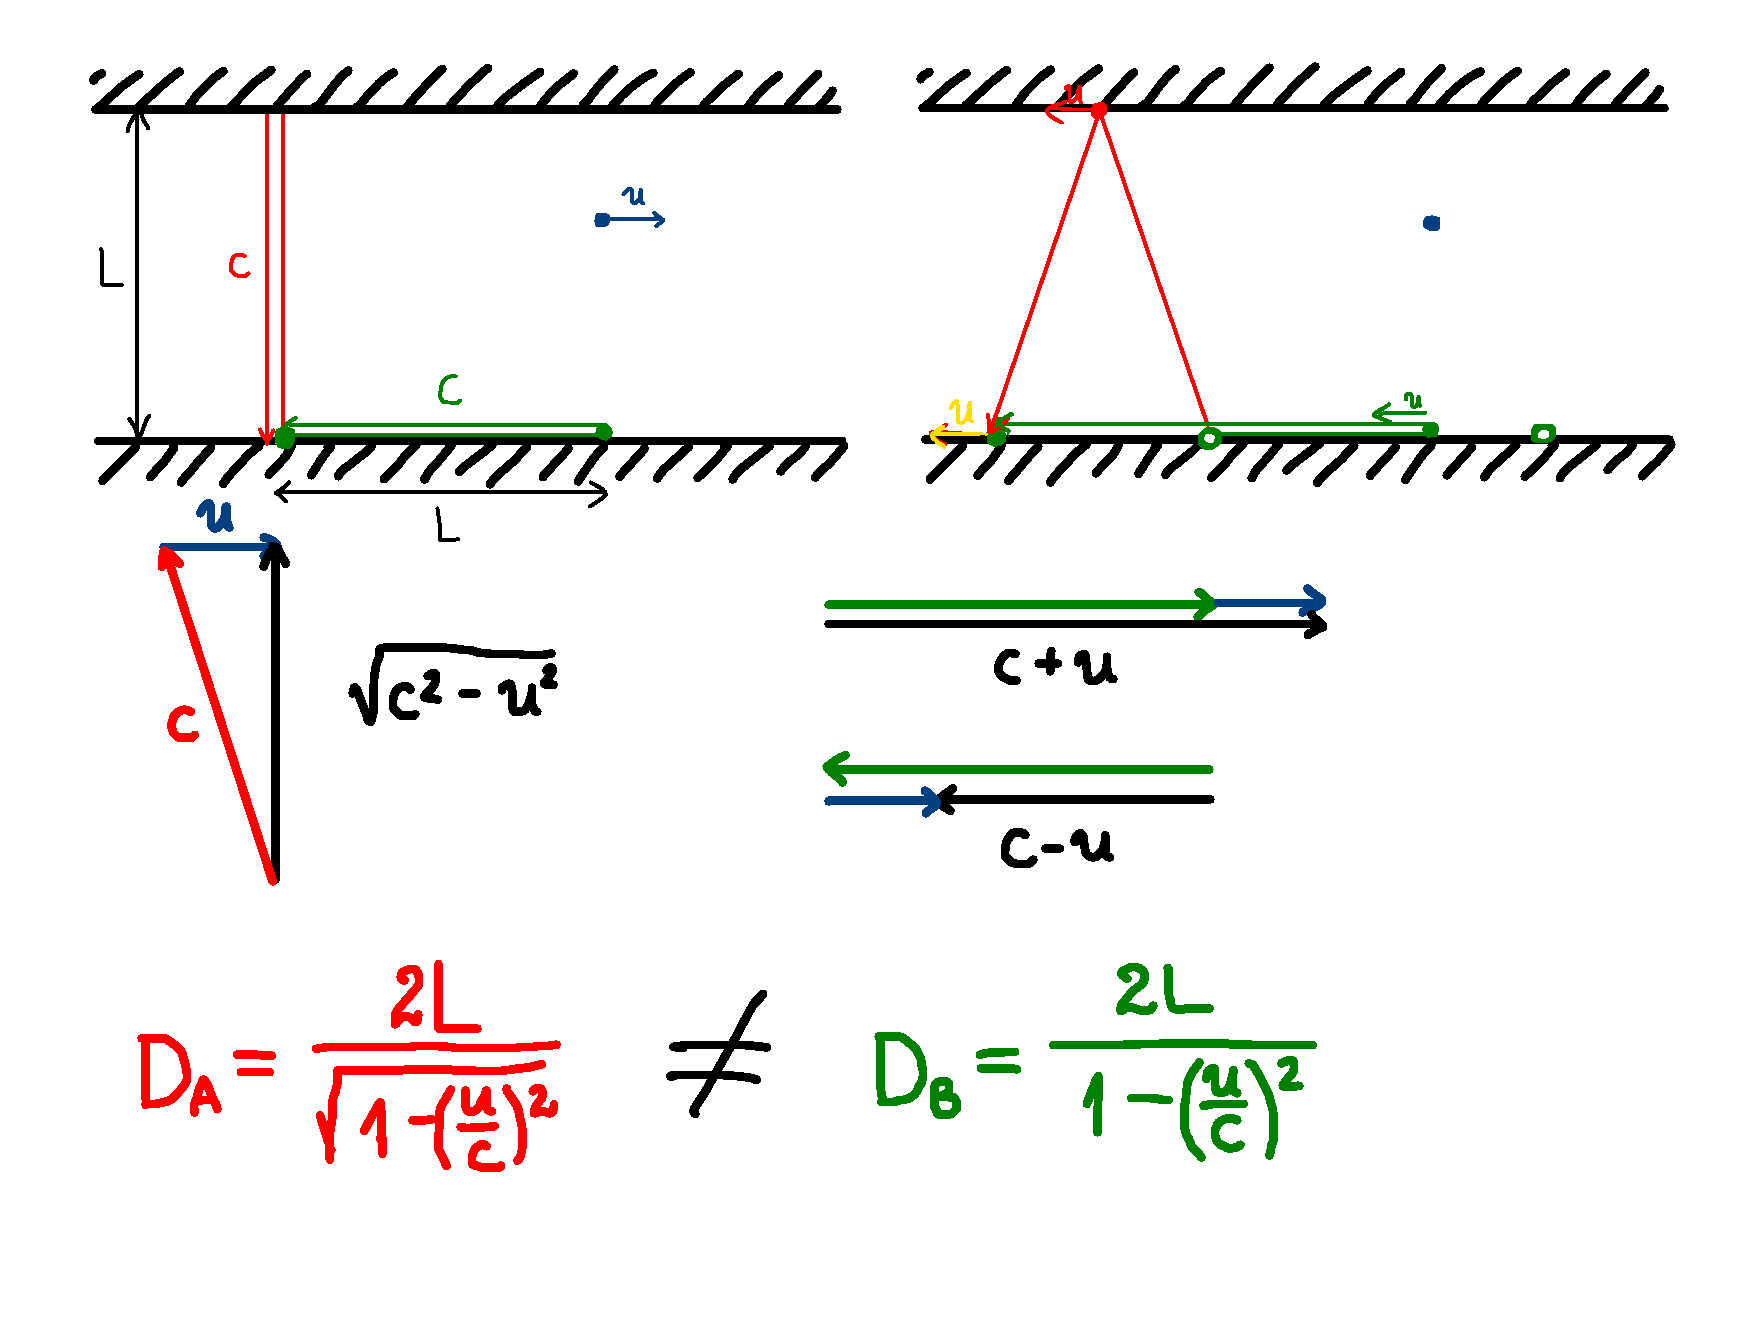
\includegraphics[width=1\linewidth]{pages/STA-page11}
Oderwijmy się na chwilę od elektromagnetyzmu i wykonajmy pewien eksperyment myślowy.
Wyobraźmy sobie dwóch wioślarzy płynących w rzece, której nurt ma prędkość $u$.
Obaj starują z tego samego punktu i płyną w wodzie z tą samą szybkością $c$.
Jeden z nich płynie do punktu na drugim brzegu na tej samej wysokości rzeki i z powrotem.
Drugi płynie na jednakową odległość wzdłuż brzegu. Najpierw w dół, a potem w górę rzeki.

Aby nie zostać zniesionym przez nurt, pierwszy z nich musi skierować
łódkę nieco przeciwnie do nurtu rzeki. Używając geometrii widzimy,
że składowa prędkości prostopadła do brzegu będzie wynosić $\sqrt{c^2-u^2}$.
Efektywna droga, którą przebył względem wody wynosi więc:
\[
  \mathcolor{BrickRed}{D_A}
  = c \mathcolor{BrickRed}{t_A}
  = c \frac{2L}{\sqrt{c^2-u^2}}
  = \frac{2L}{\sqrt{1 - (u/c)^2}}.
\]

Drugi wioślarz jest w nieco innej sytuacji. Najpierw wiosłuje z prądem, więc
płynie szybciej $c + u$, ale wraca pod prąd i płynie wolniej $c - u$.
Dla niego również możemy policzyć efektywną przebytą drogę:
\[
  \mathcolor{ForestGreen}{D_B}
  = c (\mathcolor{ForestGreen}{t_{B1}} + \mathcolor{ForestGreen}{t_{B2}})
  = c \left(\frac{L}{c+u} + \frac{L}{c-u}\right)
  = \frac{2L}{1 - (u/c)^2}
\]

Już na pierwszy rzut oka widać, że wartości nie są sobie równe.
Różnią się o czynnik $1 / \sqrt{1-(u/c)^2}$. Drugi wioślarz efektywnie
przebył dłuższą trasę i dotarł później.
Analizę można teraz przeprowadzić do tyłu i znając różnicę przebytych odległości
wyznaczyć szybkość z jaką płynie woda w rzece.

Myślę, że już domyślasz się co mają wioślarze wspólnego z elektromagnetyzmem.
Ten sam eksperyment można przeprowadzić używając światła i luster,
gdzie nurt rzeki to płynący eter. Taki eksperyment został przeprowadzony
przez Alberta Michelsona i Edwarda Morleya pod koniec XIX w.
\newpage

\noindent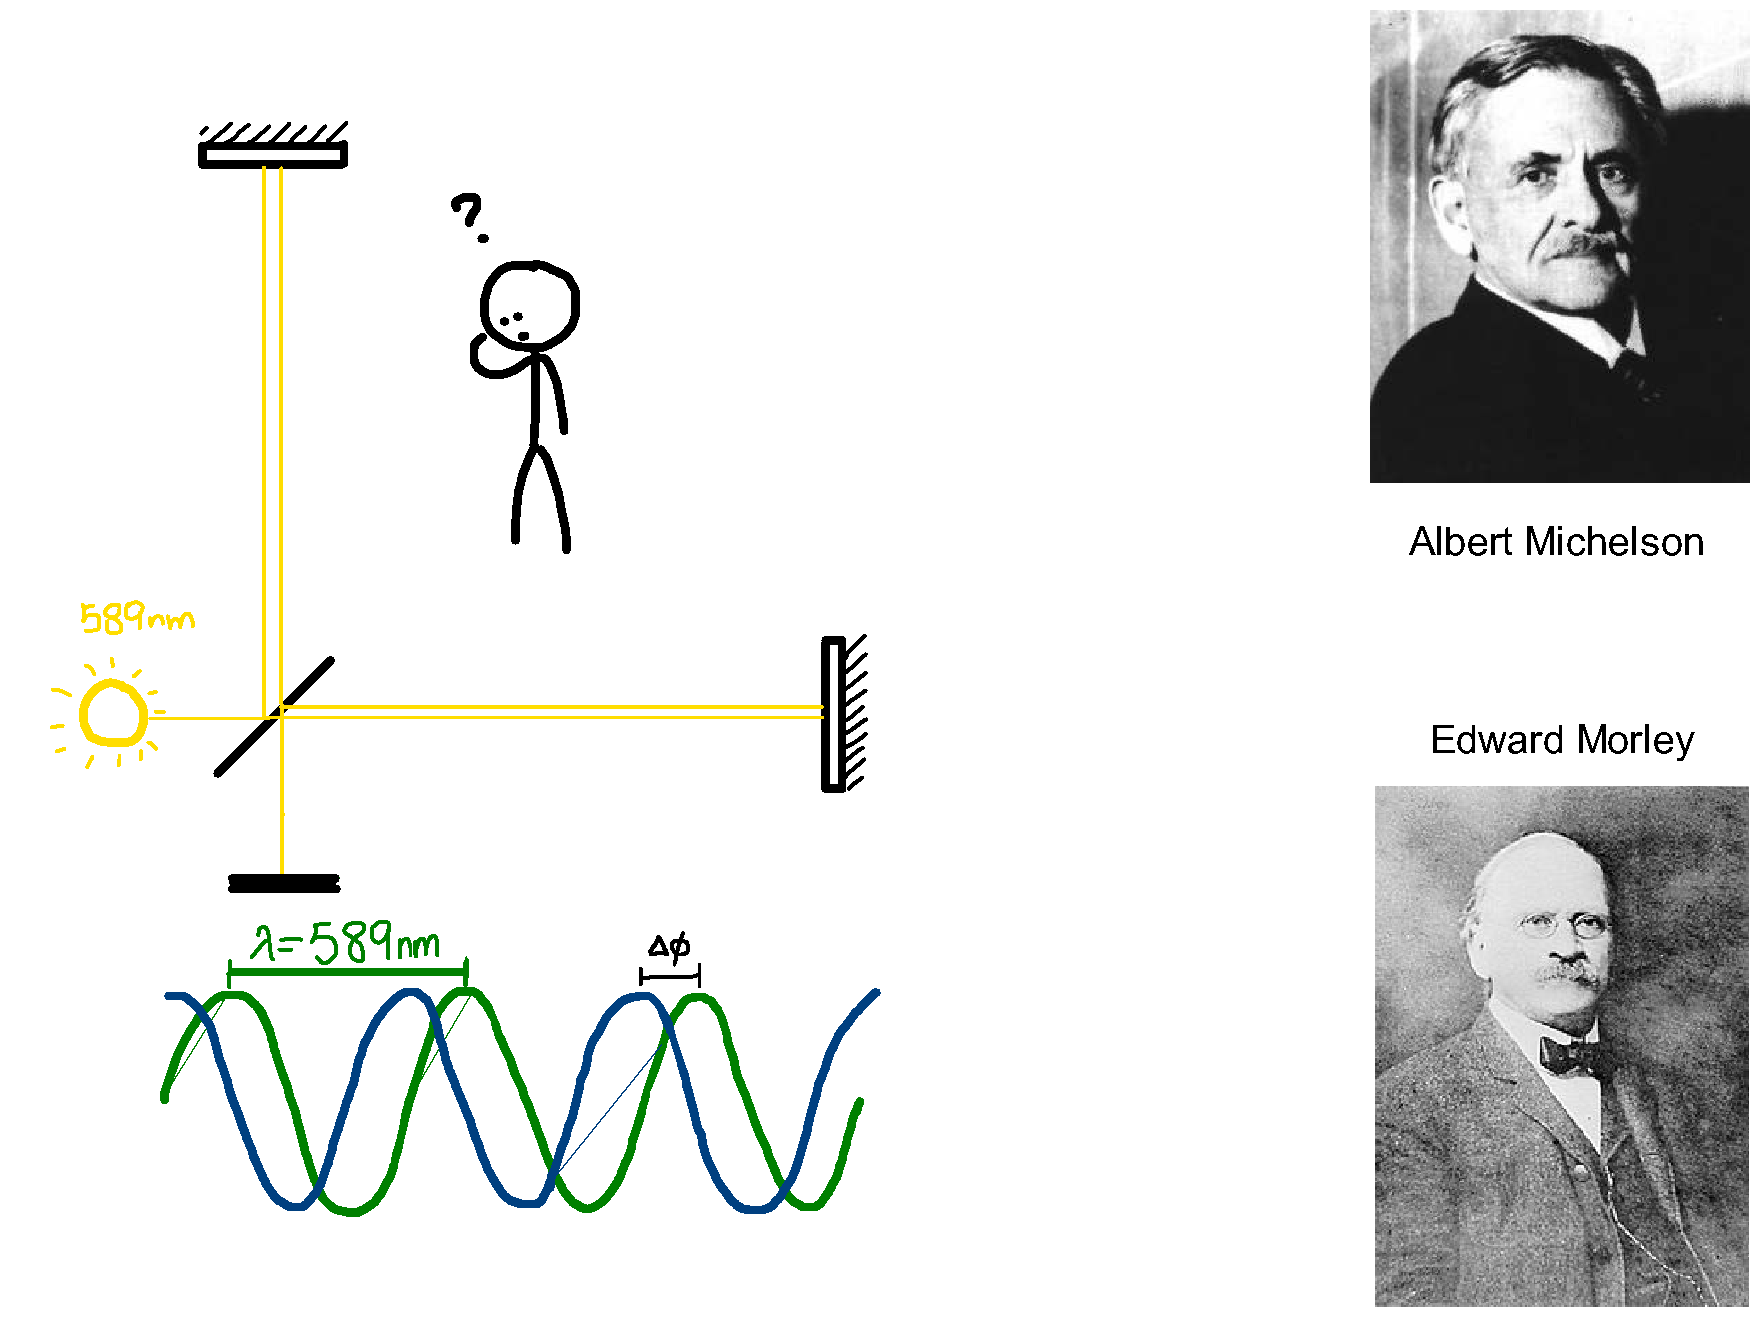
\includegraphics[width=1\linewidth]{pages/STA-page12}
Eksperyment Michelsona-Morleya, urządzenie nazwane interferometrem,
składa się ze źródła światła, płytki półprzepuszczalnej, dwóch luster i ekranu.
Światło (monochromatyczne lub białe) trafia na płytkę dzielącą,
która połowę padającego światła przepuszcza, a drugą połowę odbija pod kątem prostym.
Obie wiązki lecą wzdłuż ramion interferometru do równo oddalonych luster,
odbijają się i wracają do płytki gdzie się łączą.
Za płytką jest umieszczony ekran, na którym można oglądać interferencję dwóch wiązek.
Jeśli jedna z nich przebyłaby dłuższą drogę niż druga, będzie skutkować
to przesunięciem prążków interferencyjnych.

Zamiast pomiarów bezpośrednich, eksperyment pozwalał na pomiar odchylenia w stosunku do
długości fali światła widzialnego, około \SI{600}{\nano\metre}.
Poprzez wielokrotne odbicie światła uzyskano ramiona długości \SI{11}{\metre},
co pozwalało obserwować nawet nanometrowe odchylenia gołym okiem.

Całe urządzenie umieszczono na kamiennej płycie, która powoli obracała się
w basenie z rtęcią. Oczekiwano, że prążki będą przesuwać się
wraz z obrotem interferometru, jednak nie zaobserwowano
\textbf{żadnych} przesunięć. Wielokrotne powtarzanie eksperymentu dawało
dokładnie te same rezultaty.
\newpage

\noindent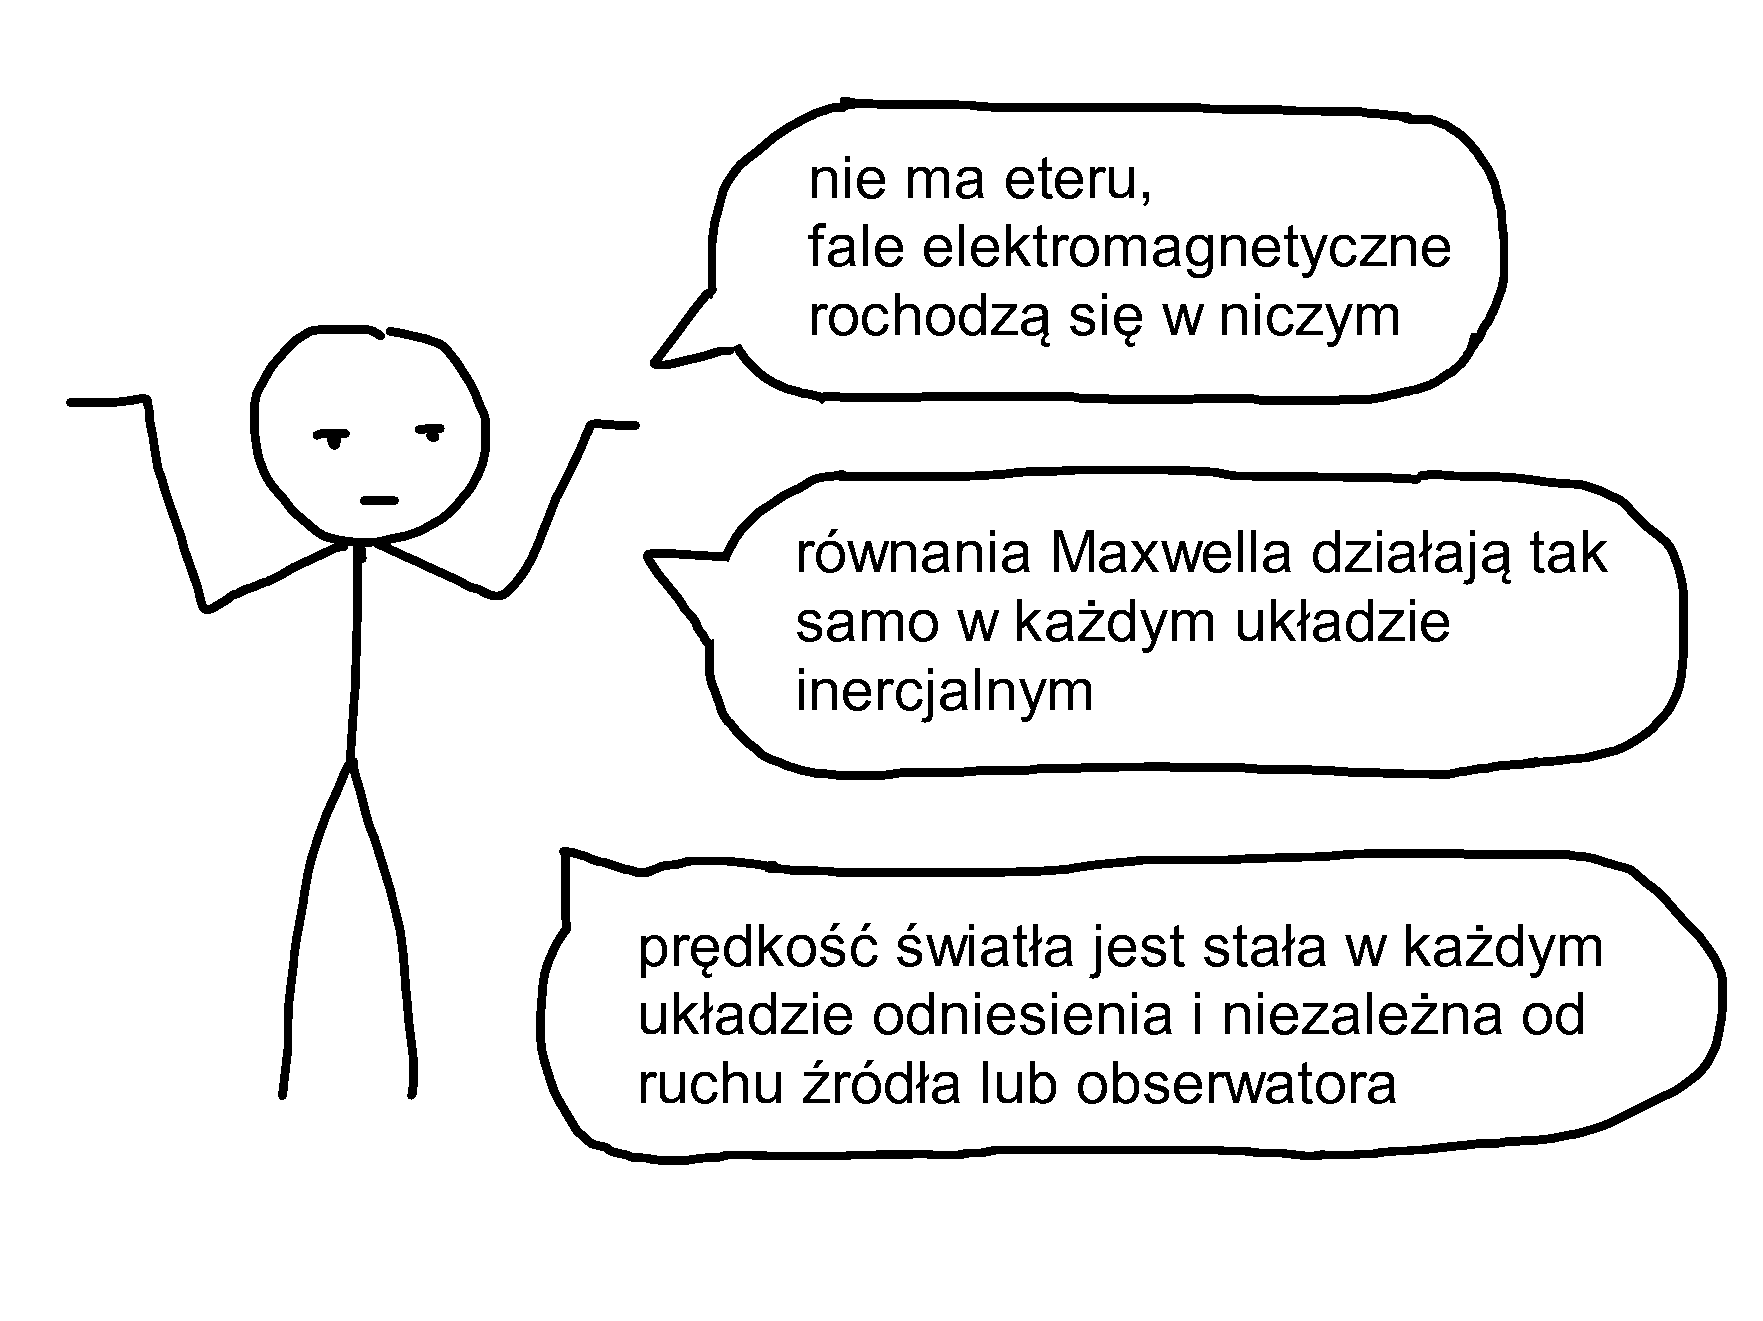
\includegraphics[width=1\linewidth]{pages/STA-page13}
Ten niewinnie wyglądający wynik eksperymentu niósł ze sobą poważne
konsekwencje, które postawiły na głowie świat fizyki.

Ponieważ eksperymenty wskazywały na brak istnienia eteru, trzeba było
przyjąć, że fale elektromagnetyczne rozchodzą się w niczym i nie ma żadnego
punktu odniesienia do mierzenia ich prędkości. Dalej, równania Maxwella
muszą być prawdziwe w każdym układzie odniesienia, bo nie ma powodu, by
którykolwiek, a w szczególności nasz ziemski był przez przyrodę faworyzowany.
Wynika więc, że każdy obserwator będzie widział taką samą prędkość światła,
niezależnie od ruchu jego samego lub źródła światła.

W tym momencie słychać już śmieciarkę jadącą po dotychczasową fizykę
opartą na obserwacjach Galileusza. Skoro $c$ dla każdego jest takie same
to znaczy, że prędkości się nie dodają, położenie i odległości nie mogą być
jednoznacznie ustalone przez różnych obserwatorów i cała kinematyka i dynamika
nadaje się do kosza.
\newpage

\noindent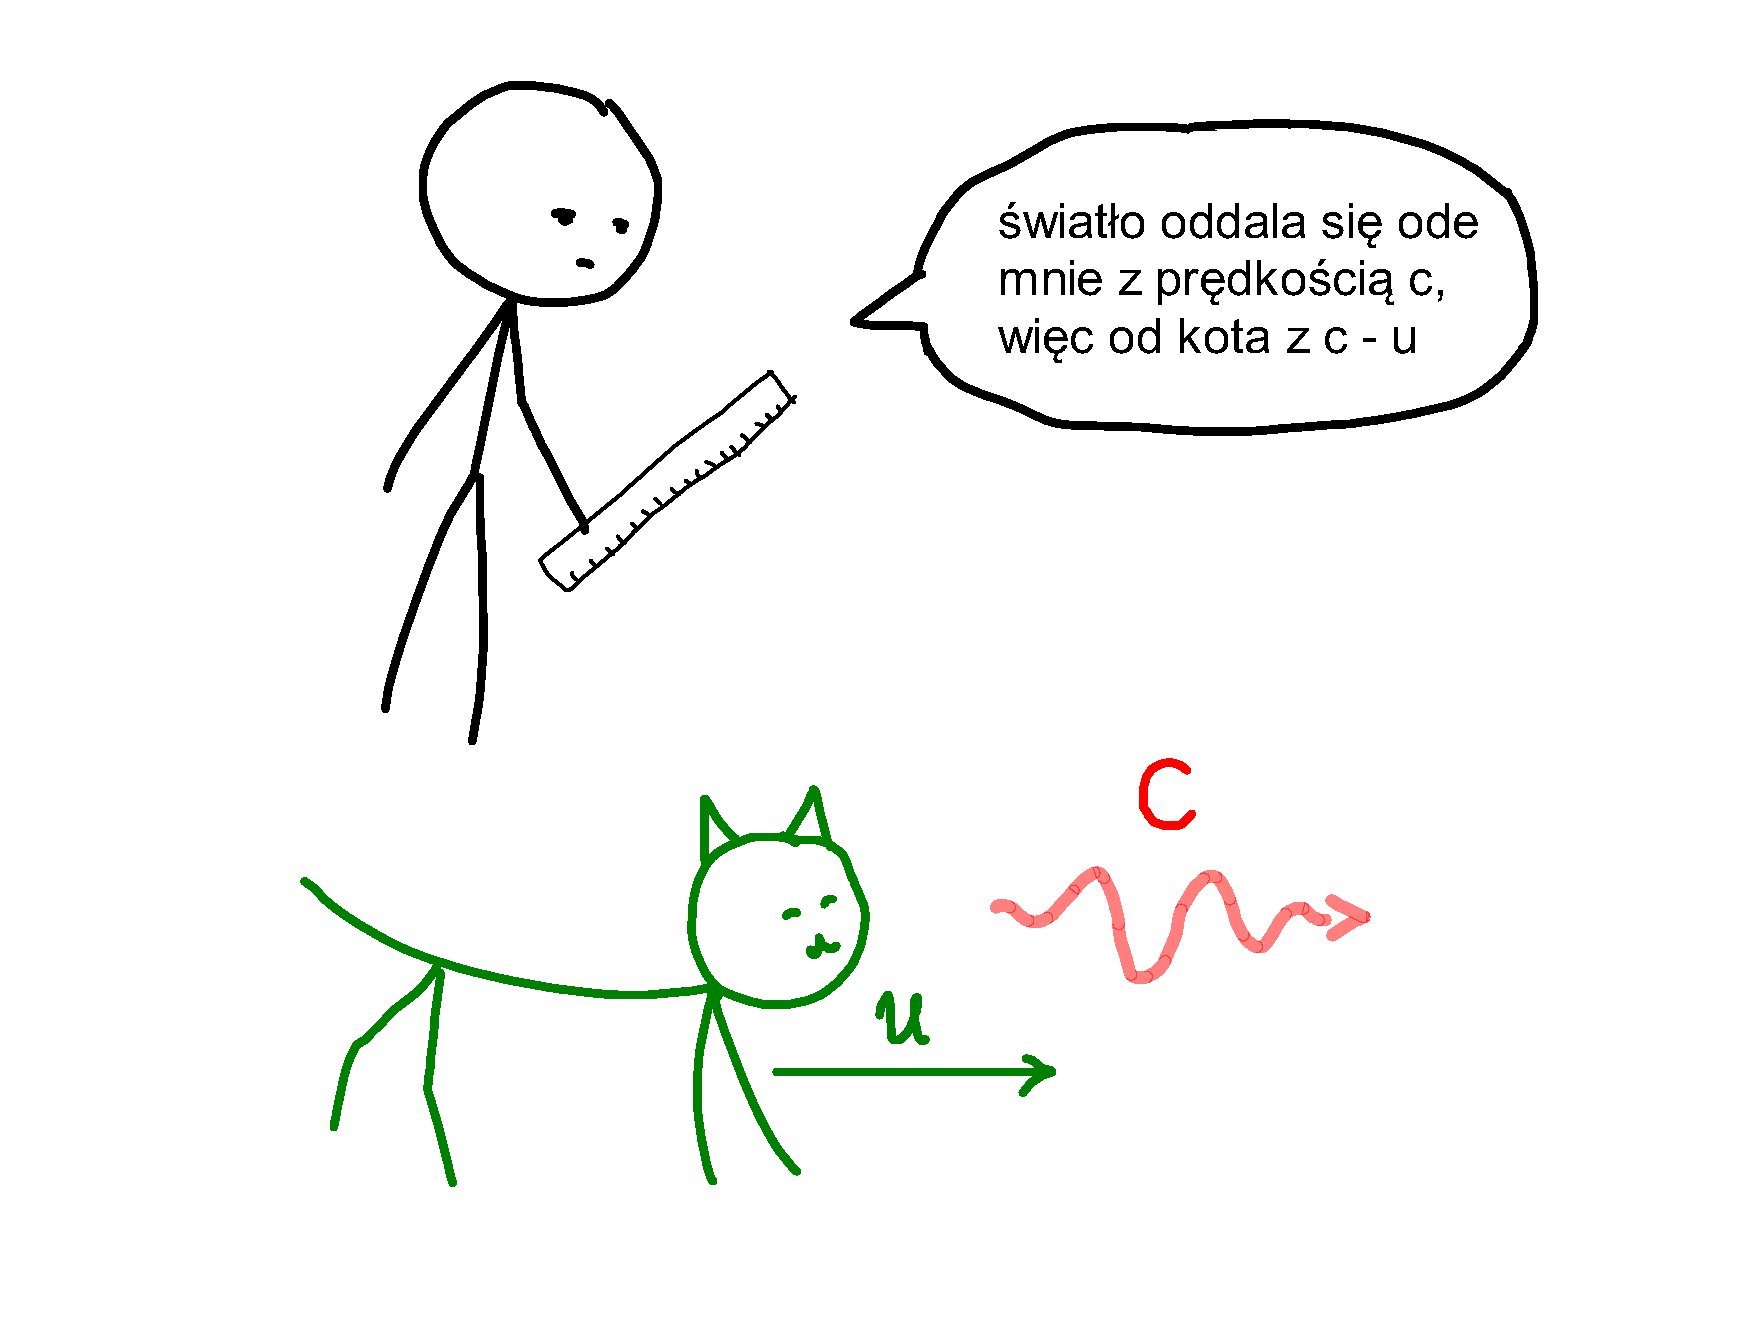
\includegraphics[width=1\linewidth]{pages/STA-page14}
Wykonajmy następujący eksperyment myślowy. Cyber-kot przebiegający obok
Alfreda, mijając go wystrzeliwuje z oczu wiązkę lasera.
Równania elektrodynamiki jasno mówią, że światło będzie oddalać się od
Alfreda w prędkością $c$. Ponieważ kot tą wiązkę goni, odległość między
kotem a wiązką będzie rosnąć z prędkością $c - u$. Co więcej, jeśli kot
będzie biegł dostatecznie szybko, to mógłby tą wiązkę nawet wyprzedzić.
\newpage

\noindent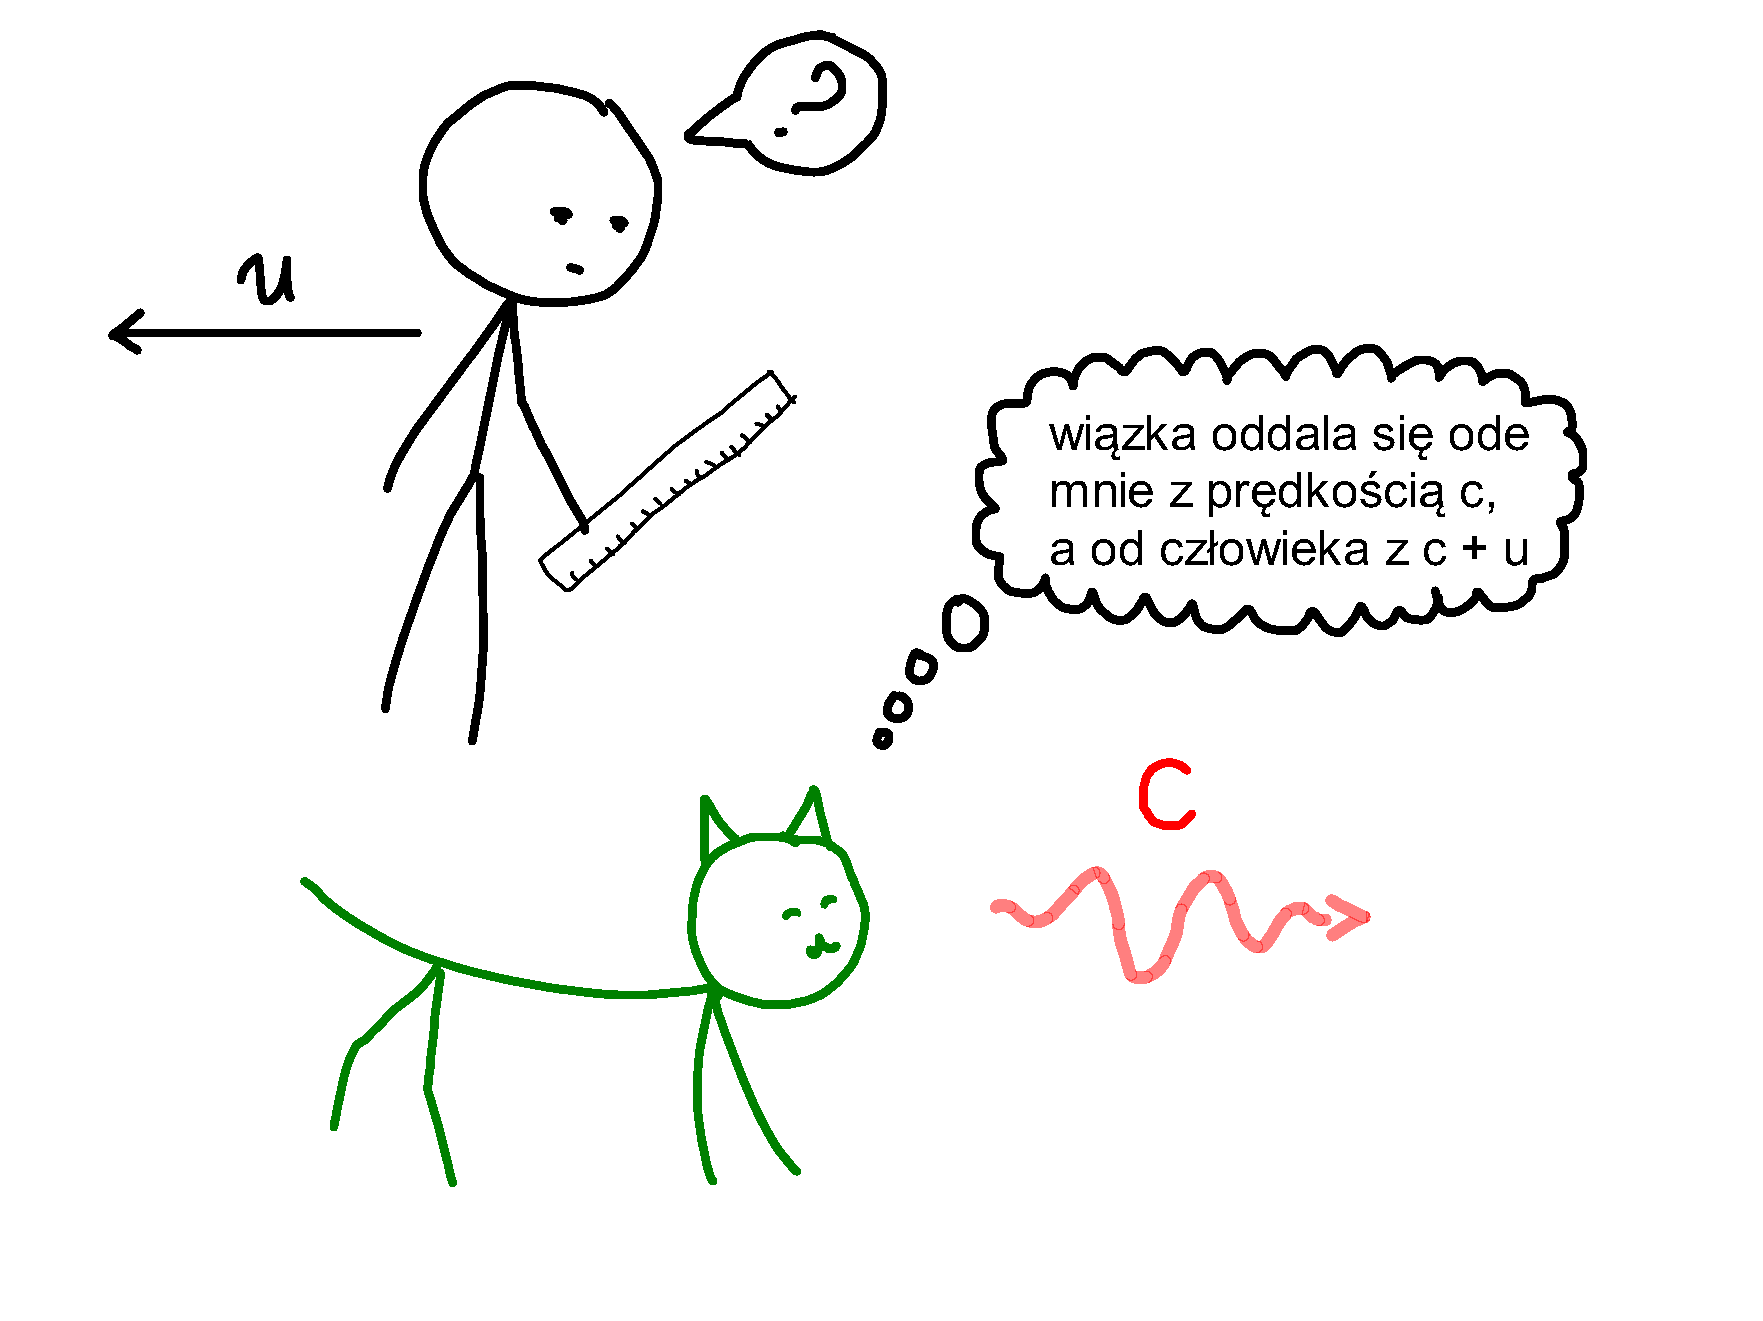
\includegraphics[width=1\linewidth]{pages/STA-page15}
A jak sytuacja wygląda z punktu widzenia kota? Podlega on dokładnie tym samym
prawom fizyki, więc w jego układzie odniesienia światło ucieka
od niego z szybkością $c$. Nie ma szans dogonić wiązki, bo będzie ona
zawsze się oddalać ze stałą prędkością.

Zdecydowanie mamy tu paradoks nie tylko z dodawaniem prędkości ale też
na podłożu przyczynowo-skutkowym. Kot nie może przegonić wiązki w jednym
układzie i zawsze zostawać w tyle w innym.
Transformacja Galileusza nie działa.
\newpage

\noindent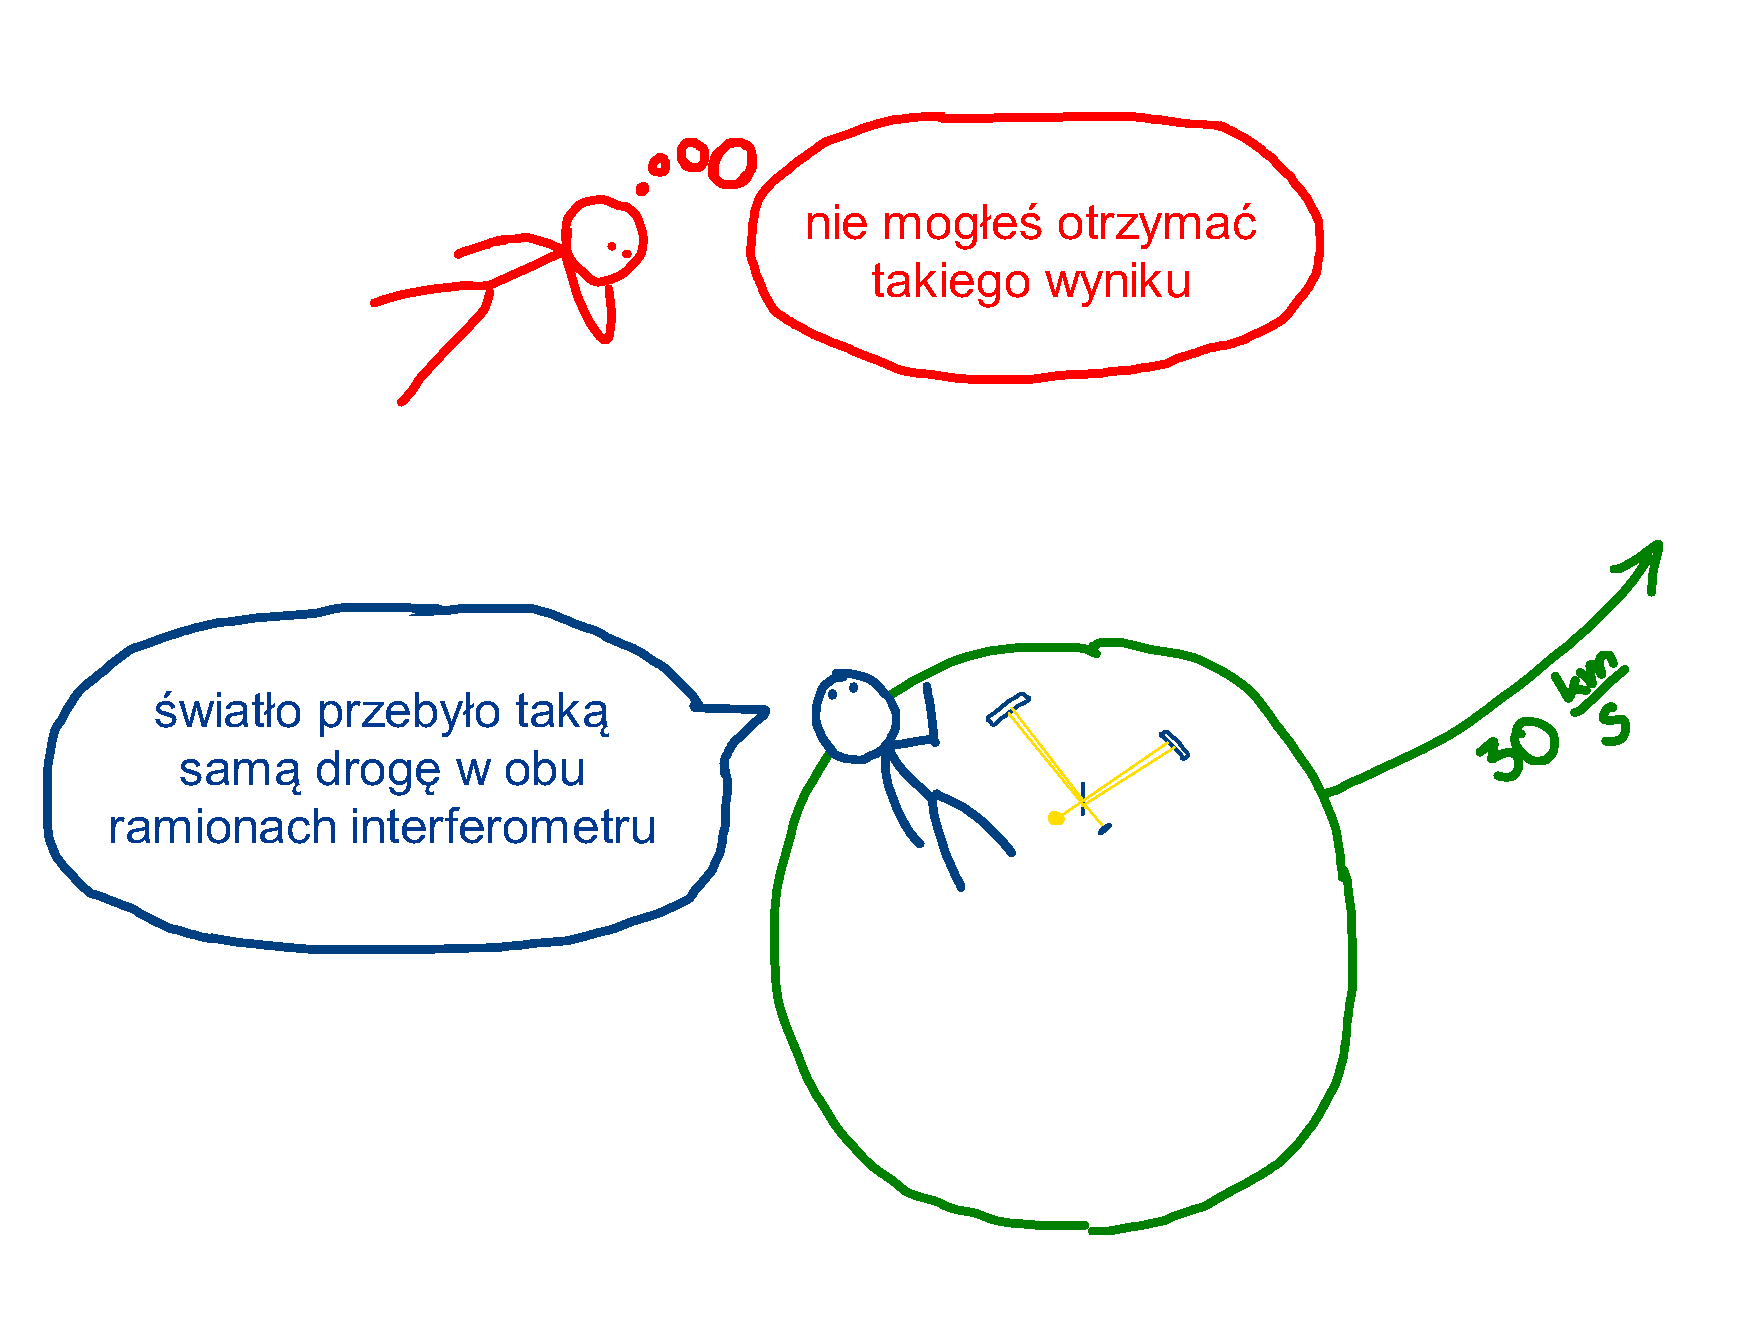
\includegraphics[width=1\linewidth]{pages/STA-page16}
Z transformacją Galileusza jest się jeszcze jeden problem.
Co zobaczyłaby Beata przyglądająca się eksperymentowi Michelsona-Morleya z kosmosu?
Michelson będąc stacjonarnym względem eksperymentu dochodzi do wniosku, że
światło w obu ramionach przebyło taką samą drogę.

Według Beaty cały eksperyment przemierza przestrzeń \SI{30}{\kilo\metre\per\second}.
Wiązka światła podróżująca wzdłuż ramienia prostopadłego do kierunku ruchu całego interferometru
przebywa pod skosem drogę ${2L}/{\sqrt{1-(v/c)^2}}$, zaś wiązka podróżująca
w ramieniu skierowanym wzdłuż kierunku ruchu najpierw goni uciekające lustro, a potem
wraca do zbliżającej się płytki dzielącej przebywając łącznie drogę
${2L}/{(1-v/c)^2}$ (patrz eksperyment z wioślarzami).
Z punktu widzenia Beaty, Michelson nie mógł nie zobaczyć przesunięcia prążków.
\newpage

\noindent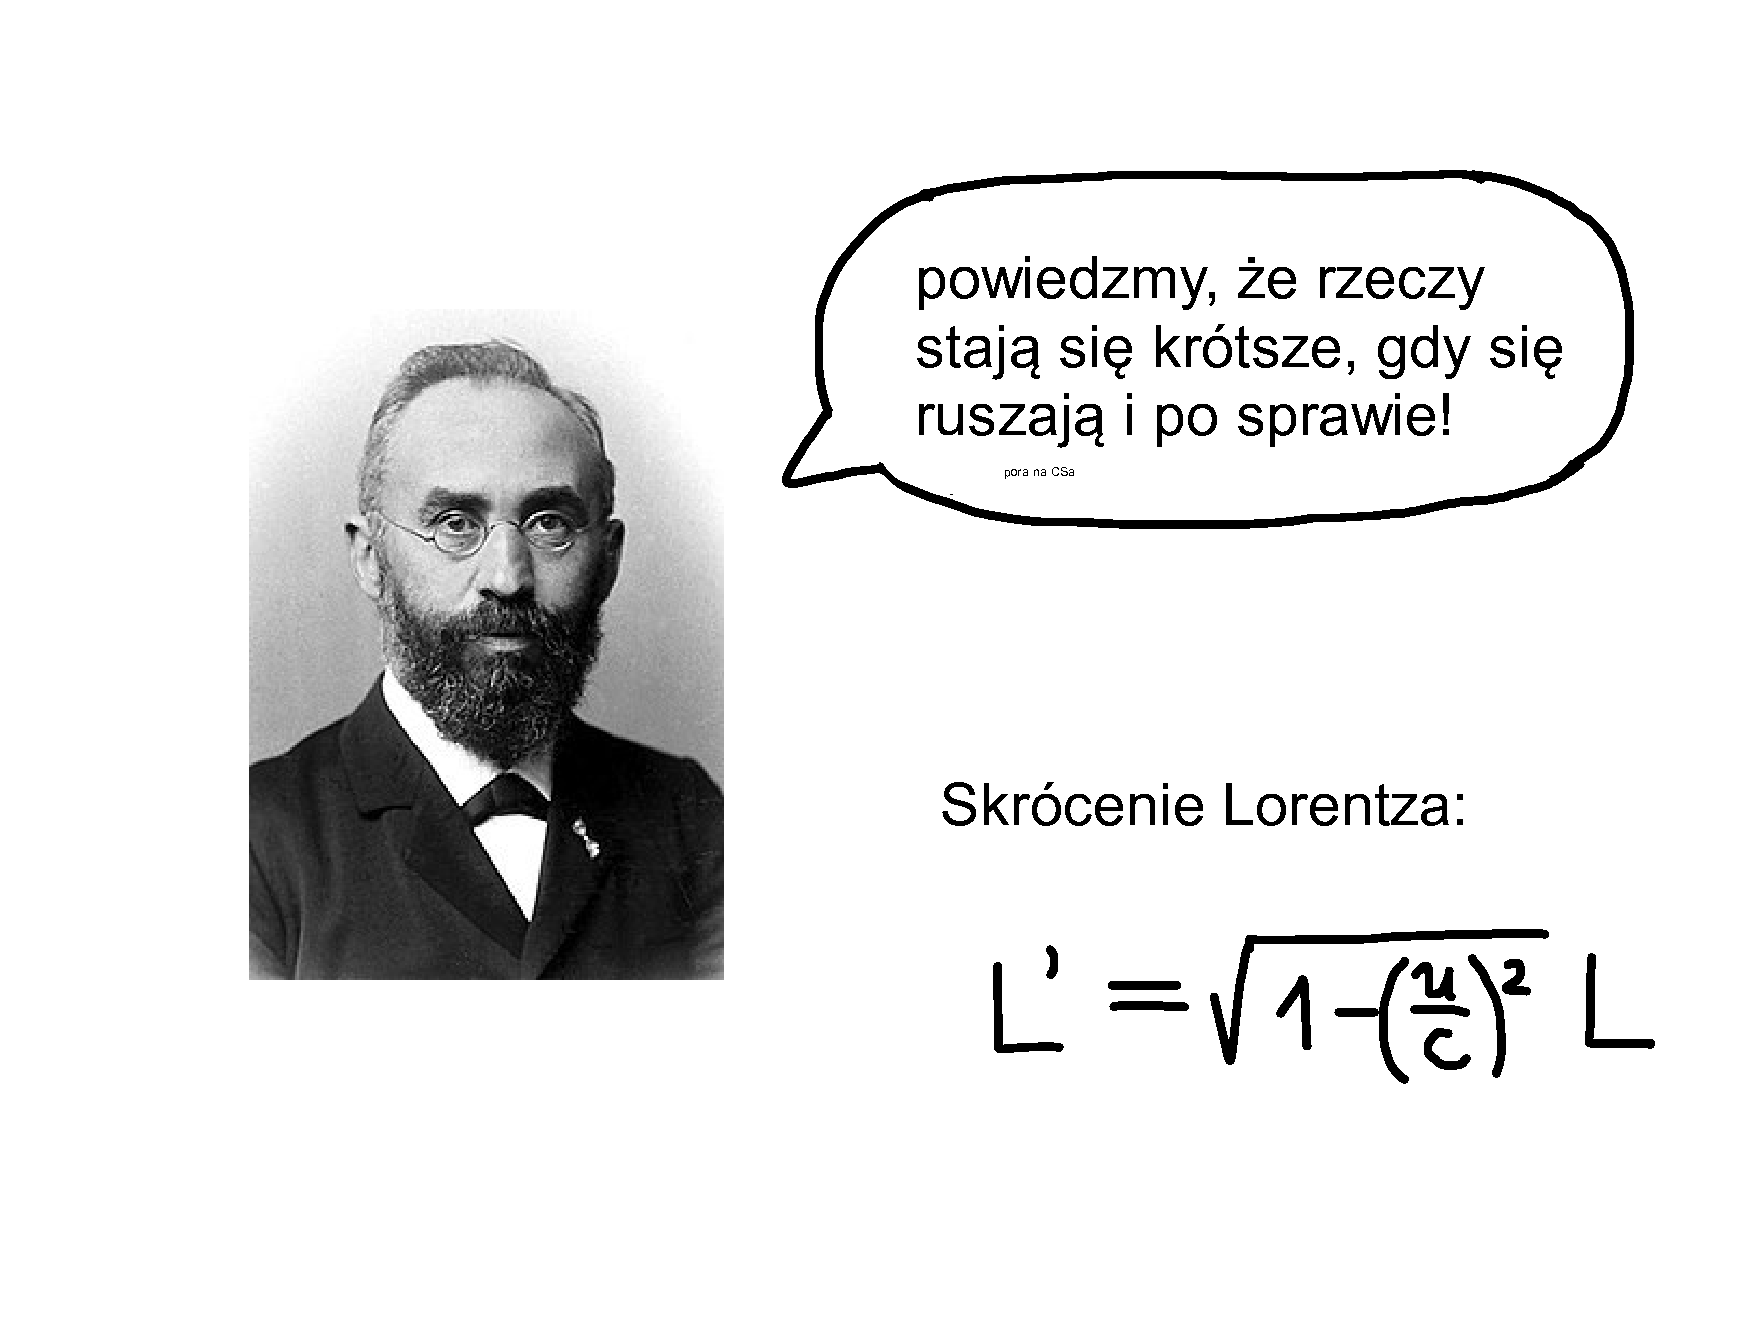
\includegraphics[width=1\linewidth]{pages/STA-page17}
Sytuację starał się ratować Hendrik Lorentz. Aby obliczenia się zgadzały, zaproponował,
aby to transformacji Galileusza dodać, że długość obiektów w ruchu zmienia się
o czynnik
\[\gamma = \frac{1}{\sqrt{1 - \left(\frac{u}{c}\right)^2}},\]
dokładnie tyle, ile wynosiła różnica drogi przebytej przez światło w ramionach
interferometru. Czynnik ten nazwano czynnikiem Lorentza, a skrócenie długości
skróceniem Lorentza.
Można było w ten sposób wyjaśnić negatywny wynik eksperymentu
Michelsona-Morleya, aczkolwiek było to bardziej załatanie dziury niż działająca
teoria.
\newpage

\noindent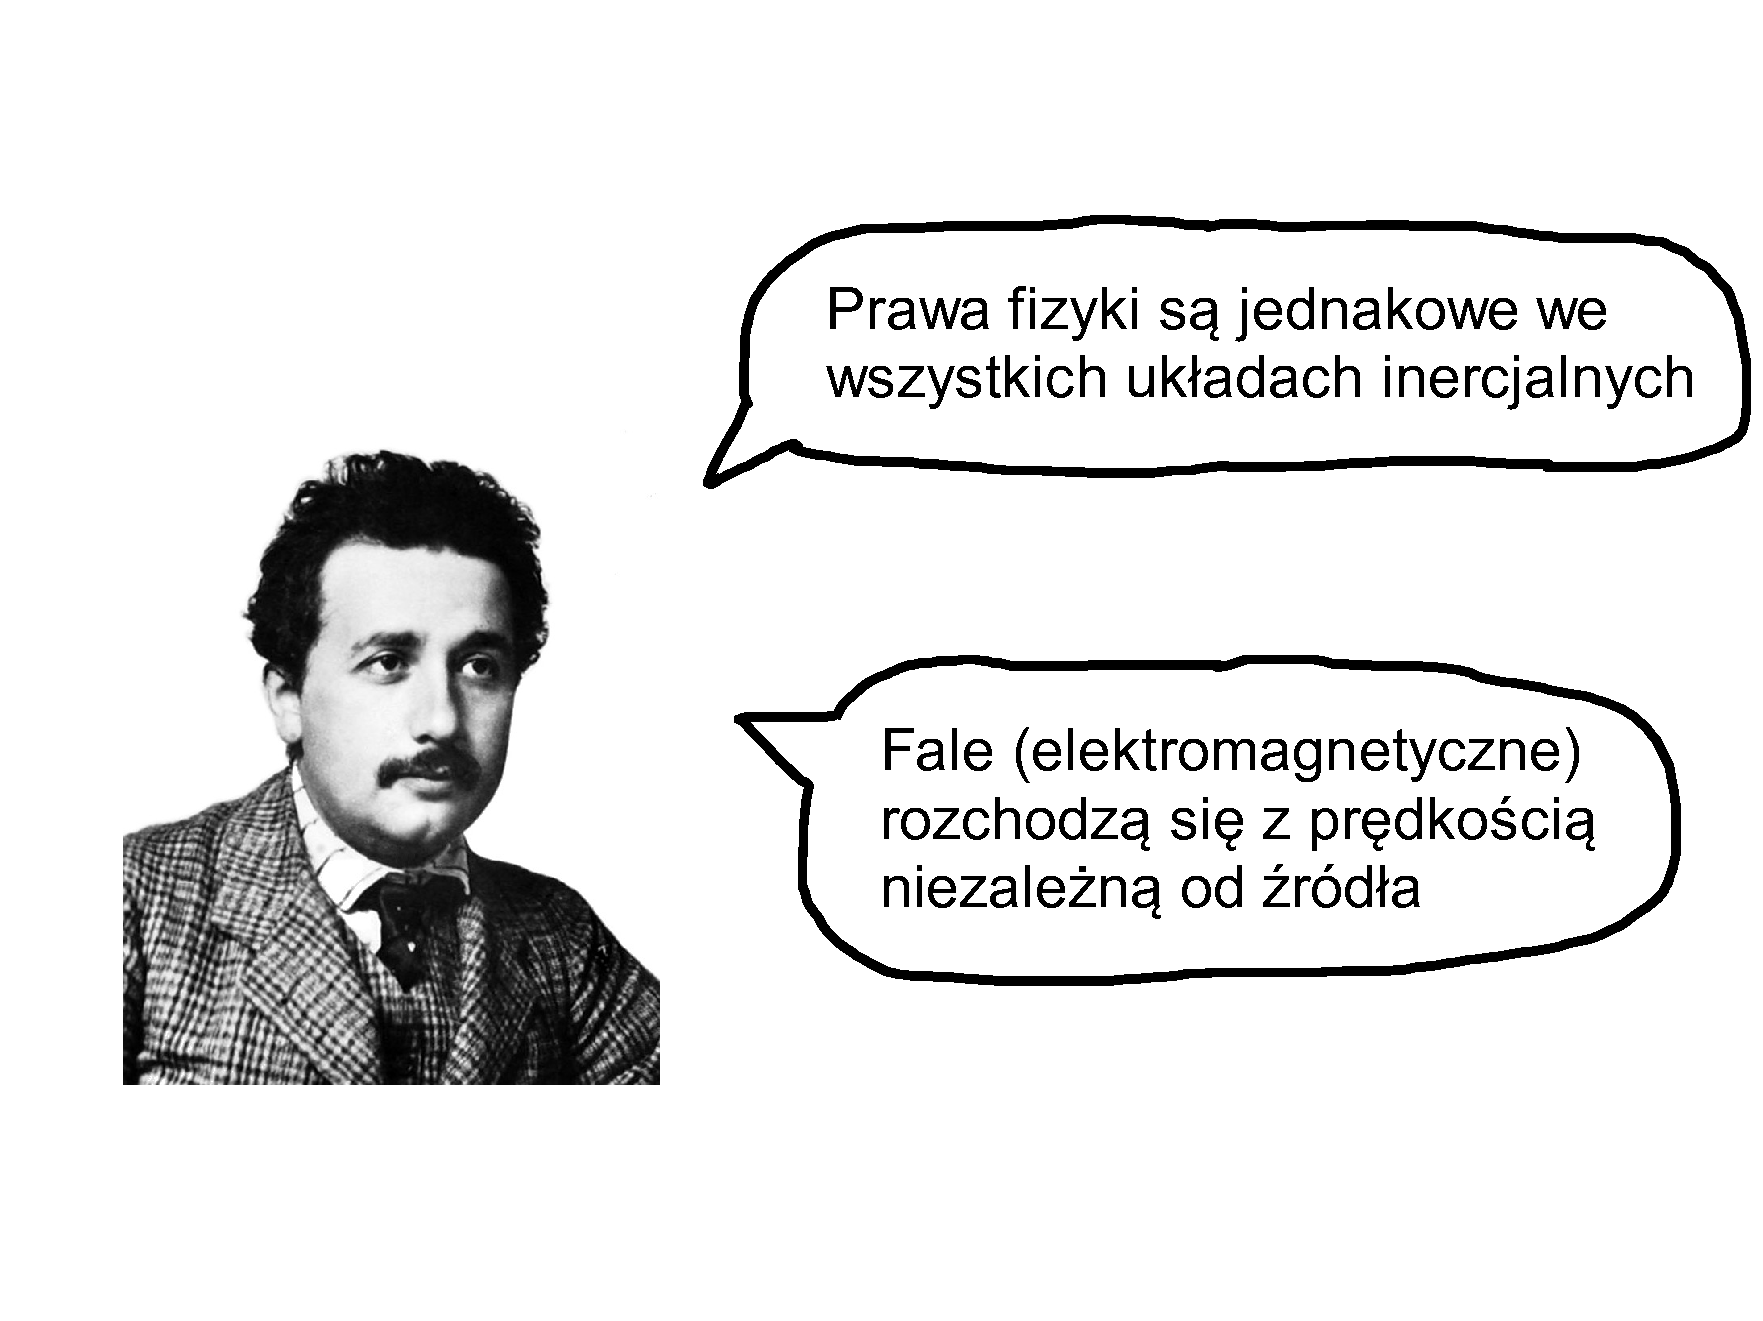
\includegraphics[width=1\linewidth]{pages/STA-page18}
Wielu fizyków, próbowało rozwikłać problem elektromagnetyzmu, jednak prawdziwy
przełom nastąpił pod wpływem nowej teorii zaproponowanej przez pewnego pracownika
szwajcarskiego urzędu patentowego.

Swoją analizę zaczął od postawienia dwóch postulatów:
\begin{enumerate}
  \item prawa fizyki są jednakowe we wszystkich układach inercjalnych,
  \item fale elektromagnetyczne rozchodzą się w próżni z niezmienną prędkością
        $c$ niezależną od źródła światła.
\end{enumerate}
Te postulaty nie wydają się niczym odkrywczym. W końcu przyroda nie faworyzuje
żadnego układu odniesienia. Niezależność prędkości fal od źródła również była
powszechnie znanym, akceptowanym i potwierdzonym eksperymentalnie zjawiskiem.
Einstein zauważył jednak, że do tego niepotrzebne jest by położenie i czas były
czymś absolutnym. Trzeba wymyślić nową fizykę, która będzie zgodna z eksperymentami
a nie odwrotnie.
\newpage

\noindent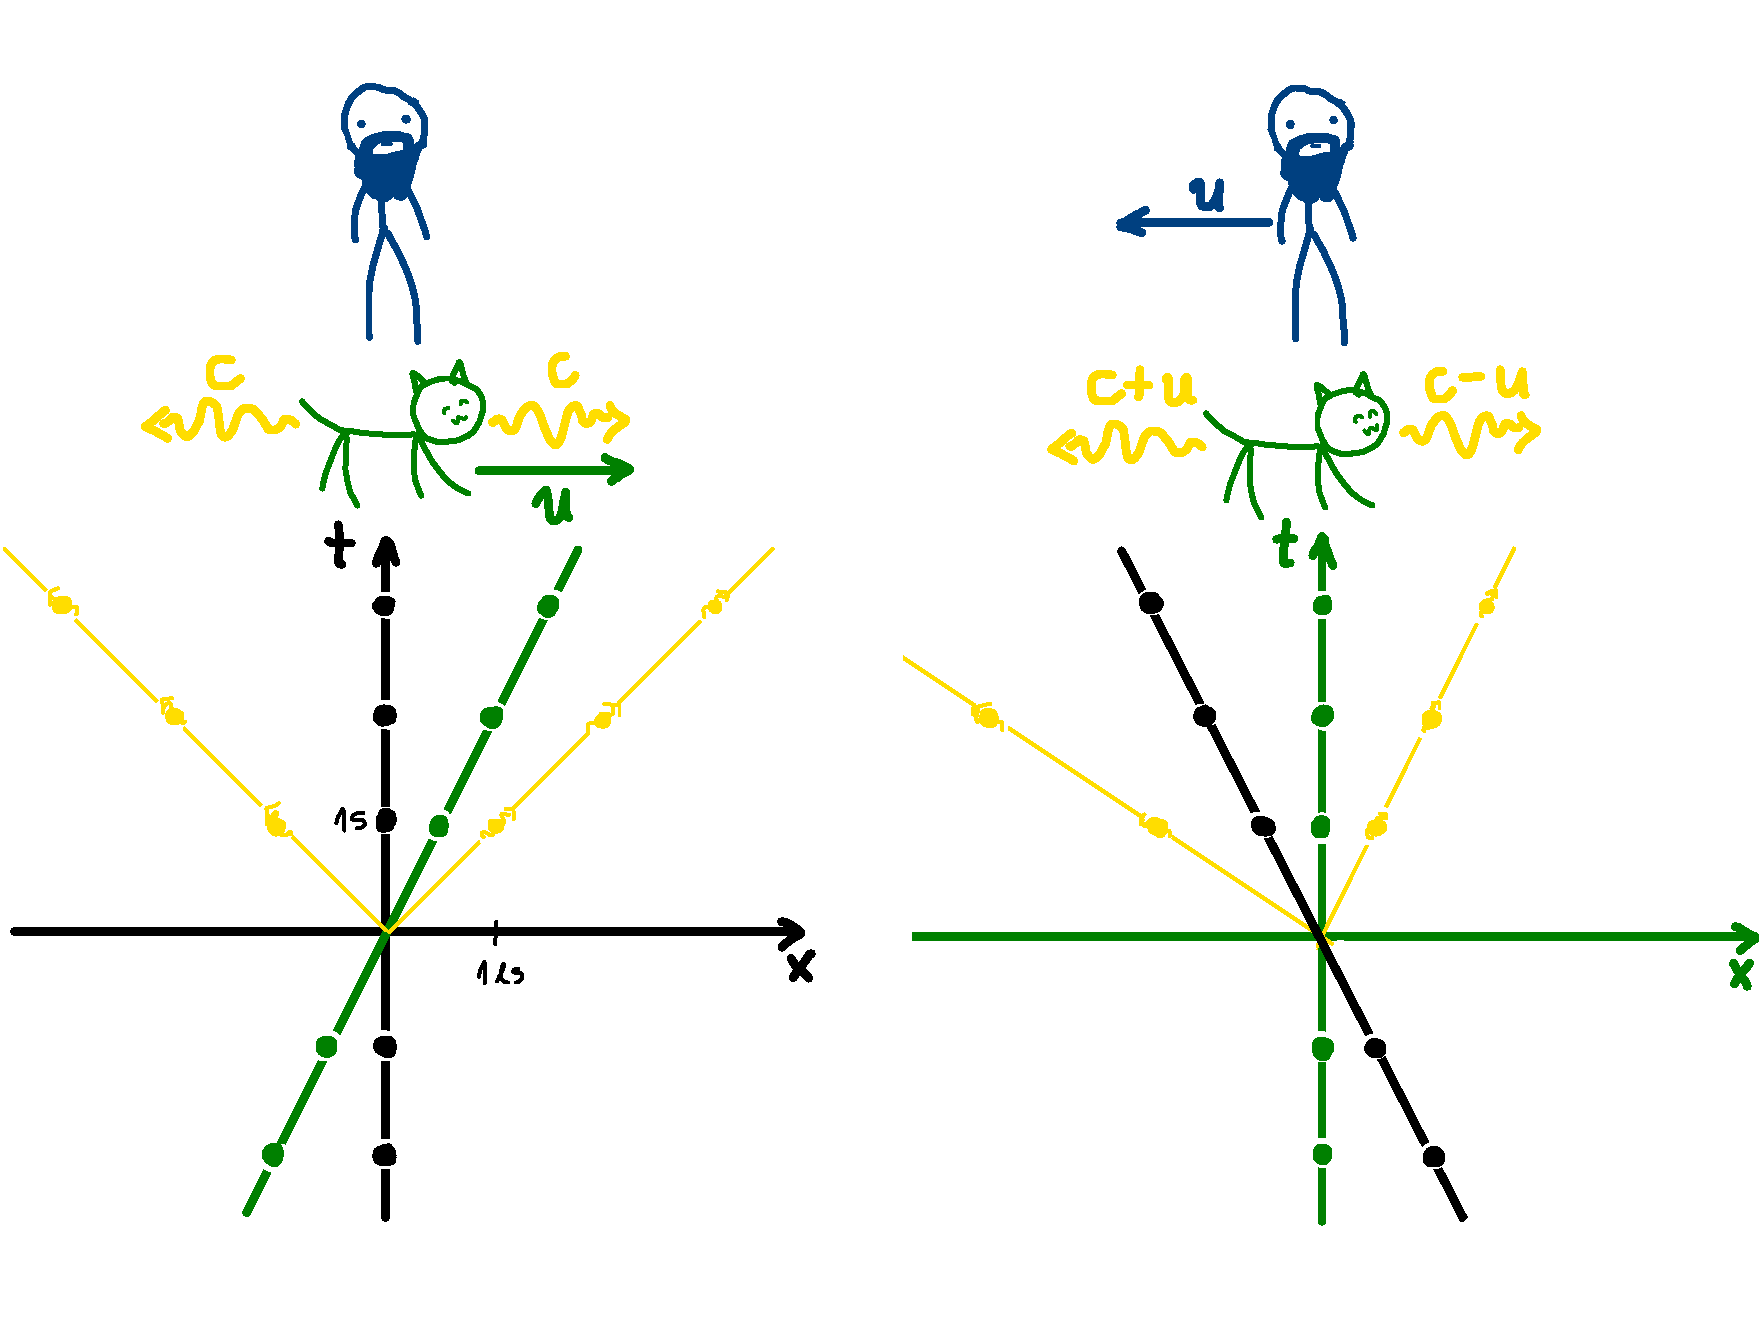
\includegraphics[width=1\linewidth]{pages/STA-page19}
Spójrzmy jeszcze raz na transformacje Galileusza, kota i lasery na diagramie
czasoprzestrzennym. Przeskalujmy osie tak, aby sekunda i sekunda świetlna miała
jednakowe długości. Wtedy linia świata dla światła będzie pod kątem \SI{45}{\degree}.
Kot, mijając Galileusza, emituje światło, które oddala się z tego punktu z
prędkością $c$ w obu kierunkach.

Jeśli przejdziemy do układu odniesienia kota używając transformacji Galileusza
(pochylenie układu tak, by linia świata kota pokrywała się z osią czasu),
widzimy, że nie zachowuje ona niezmienności prędkości światła.
\newpage

\noindent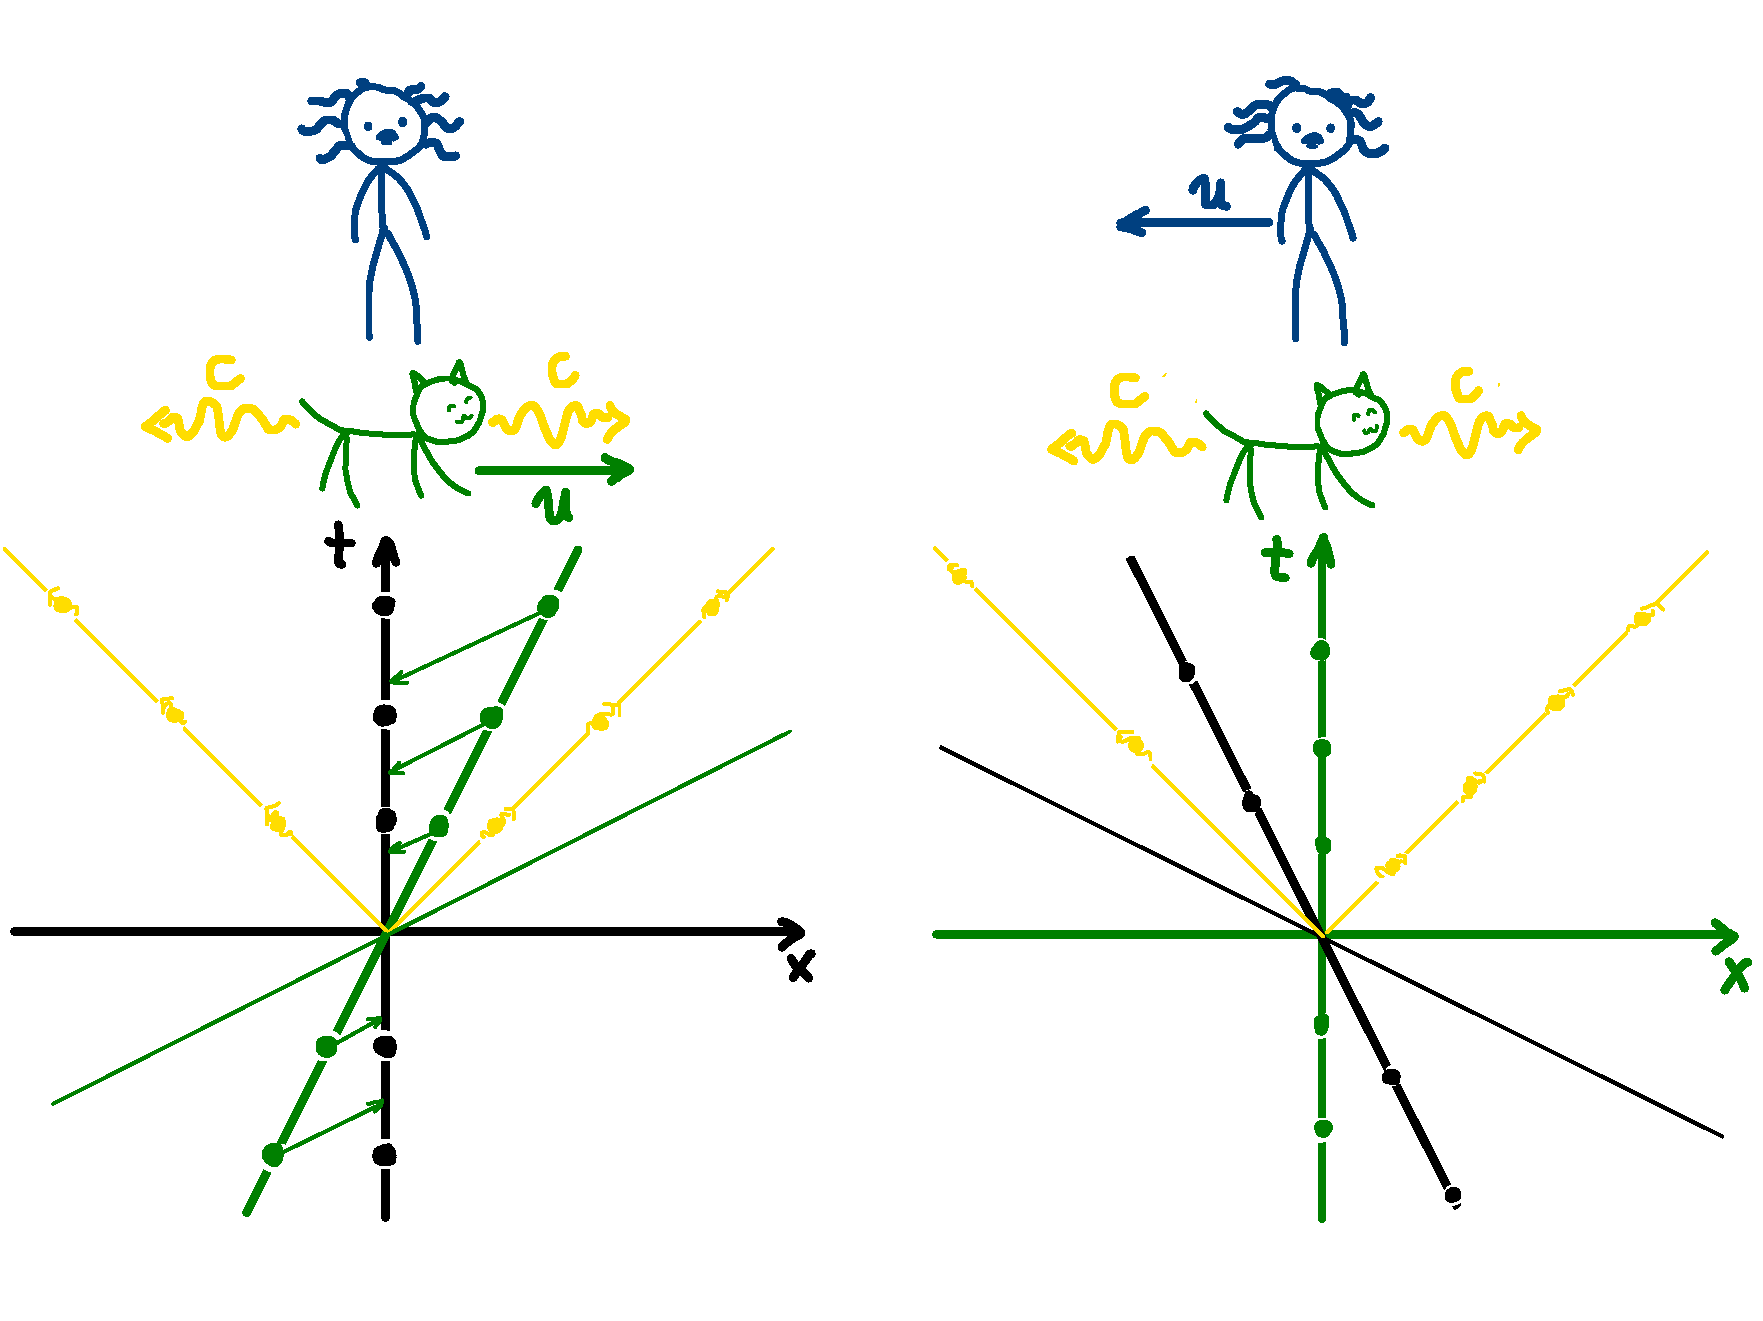
\includegraphics[width=1\linewidth]{pages/STA-page20}
Do tej pory milcząco zakładaliśmy, że czas każdego zdarzenia pozostaje niezmienny.
Wcale jednak nie musi tak być. To, że cos wydaje się nam intuicyjne, wcale nie znaczy,
że jest prawdziwe i zgodne z prawami przyrody.

Pochylenie wzdłuż osi $x$ nie jest jedyną transformacją, która pozwala zmienić układ odniesienia.
Można na przykład przesunąć punkty nie tylko wzdłuż osi przestrzennej, ale też
nieco cofnąć wzdłuż osi czasu. Taka transformacja ma jedną ciekawą właściwość, faworyzuje ona
jedną prędkość, która pozostaje niezmienna podczas przechodzenia między układami.
Pozostaje teraz wyznaczyć parametry transformacji tak, aby nie zmieniała prędkości światła.
\newpage

\noindent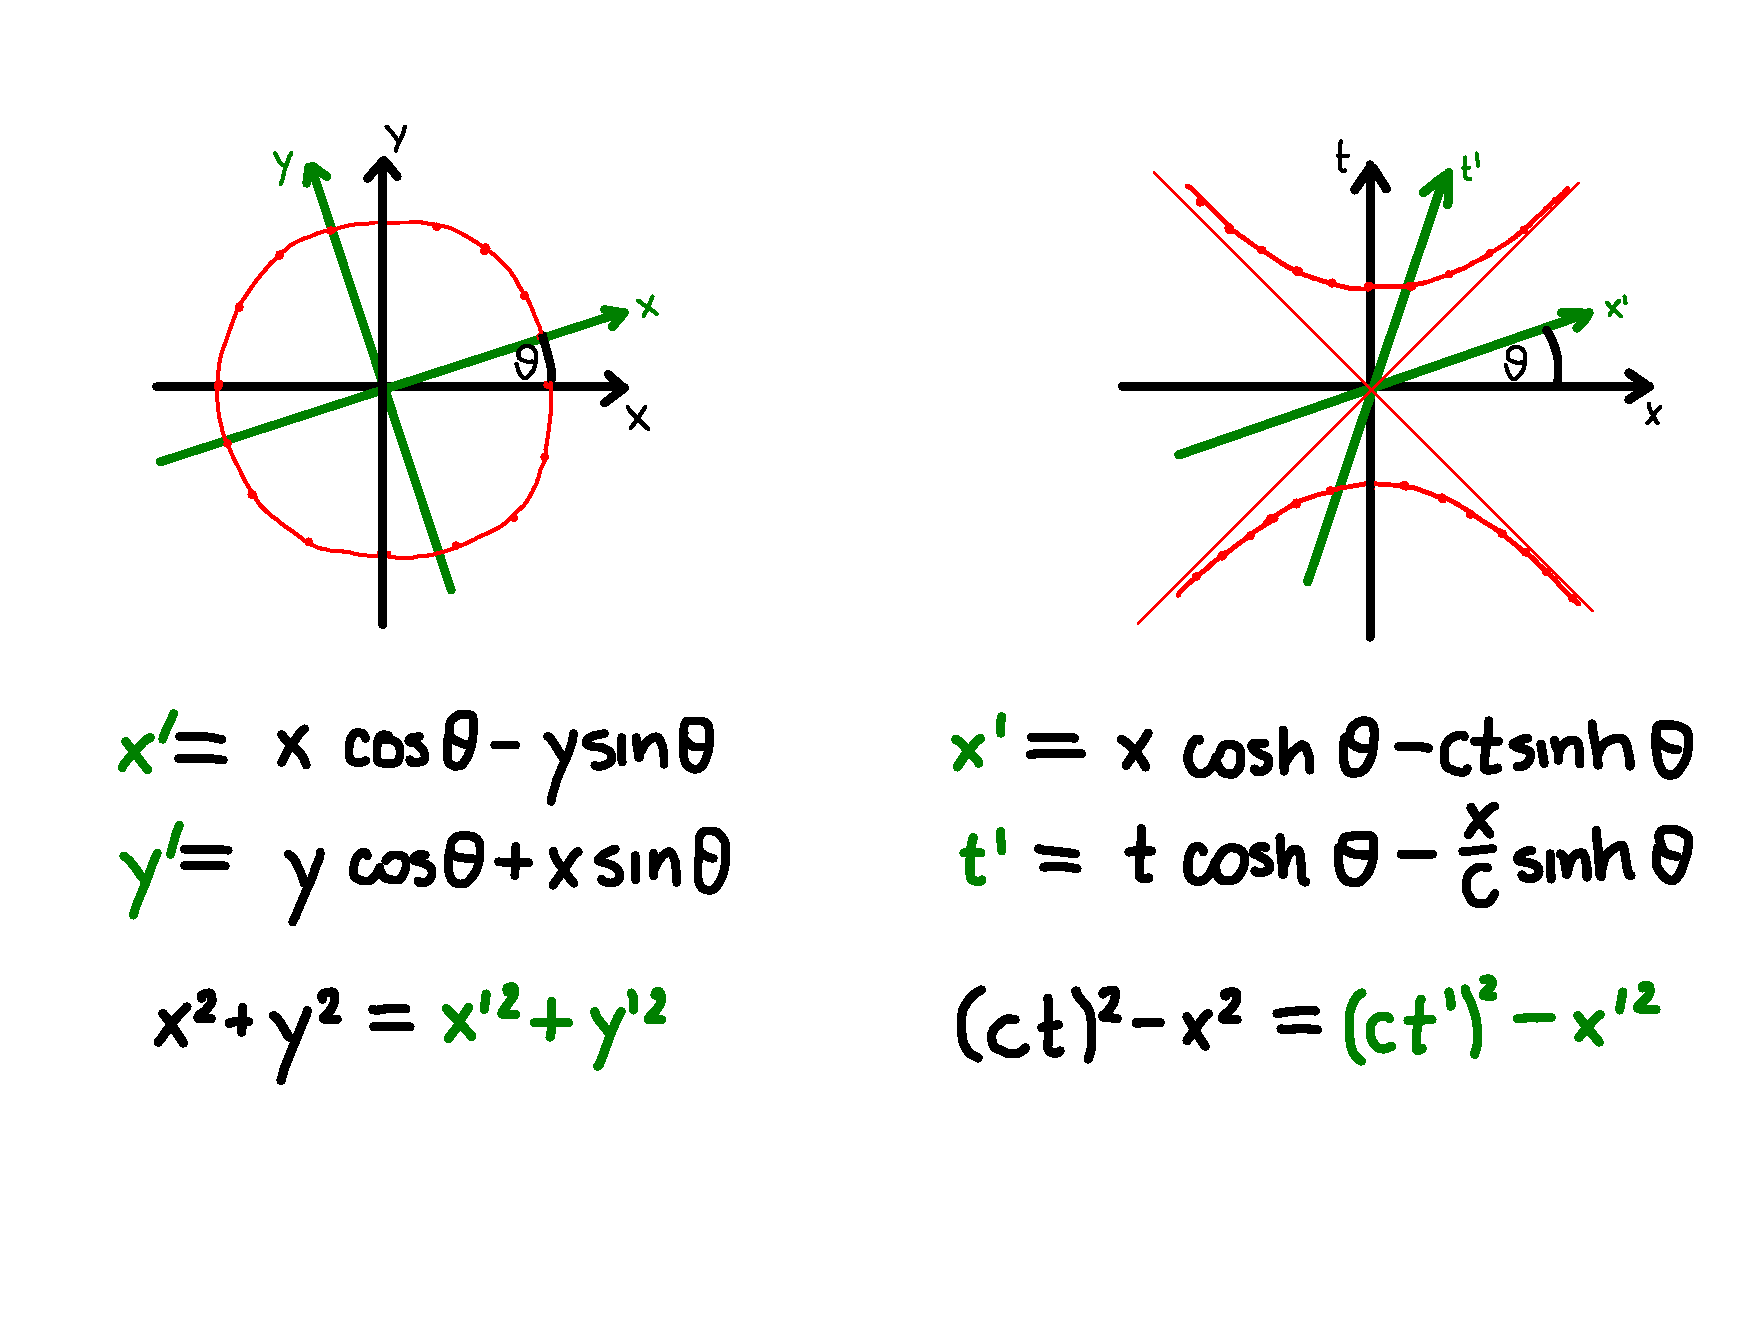
\includegraphics[width=1\linewidth]{pages/STA-page21}
Transformacja ta nosi nazwę obrotu hiperbolicznego. Nie jest ona obrotem w
tradycyjnym tego słowa znaczeniu, ale matematycznie ma wiele własności podobnych
to tych związanych z obrotem.

W przypadku klasycznego (kołowego) obrotu, punkty przemieszczają się po okręgu.
Nowe współrzędne można wyznaczyć funkcjami trygonometrycznymi
\[
  \begin{eqsystem}
    \mathcolor{Green}{x'} = x \cos\theta - y\sin\theta \\
    \mathcolor{Green}{y'} = x \sin\theta + y\cos\theta
  \end{eqsystem}.
\]

Własności okręgu gwarantują nam, że odległość każdego punktu od środka okręgu pozostaje
niezmienna, co można również wyprowadzić z powyższego równania
\[{\mathcolor{Green}{x'}}^2 + {\mathcolor{Green}{y'}}^2 = x^2 + y^2.\]

Analogicznie, podczas obrotu hiperbolicznego\footnotemark, punkty
przemieszczają się po hiperboli.
Nowe współrzędne można policzyć przy pomocy funkcji hiperbolicznych, które
noszą te same nazwy to ich trygonometryczne odpowiedniki z literą "h"
\[
  \begin{eqsystem}
    \mathcolor{Green}{ct'} = ct \cosh\vartheta - x \sinh\vartheta \\
    \mathcolor{Green}{x'} = -ct \sinh\vartheta + x \cosh\vartheta
  \end{eqsystem}.
\]

Podobnie jak ruch po okręgu zachowuje odległość od jego środka tak własności hiperboli
gwarantują nam, że leżące na niej punkty spełniają równanie
\[(\mgreen{ct'})^2 - {\mgreen{x'}}^2 = (ct)^2 - x^2.\]
W szczególności, punkty leżące na asymptocie hiperboli zawsze na niej pozostają.
Oznacza to, że linia świata wiązki światła na diagramie czasoprzestrzennym będzie
zawsze pochylona pod tym samym kątem
(będzie miała tą samą prędkość względem każdego obserwatora).

Na potrzeby równań konieczne było przeskalowanie współrzędnej $t$, co wyjaśnimy za chwilę.

\footnotetext{Kąt $\theta$ na diagramie jest kątem pochylenia osi, a nie
  matematyczną definicją kąta hiperbolicznego.}

Mamy już za sobą część matematyczną i interpretację geometryczną.
Jak możemy dojść do tego po fizycznemu?

Zacznijmy od nakreślenia wymagań jakie musi spełniać wzór na przejście do
poruszającego się układu współrzędnych.
Po pierwsze, nie może on się zmieniać pod wpływem przesunięcia zarówno w czasie jak
i przestrzeni. Wykonanie tego samego eksperymentu na Marsie albo 100 lat później
nie powinno dawać innych rezultatów. Wynika z tego, że transformacja musi być liniowa\footnotemark
\[x'= Ax + Bt.\]
\footnotetext{Liniowość transformacji Lorentza uzasadniam w dodatkach.}
Parametry $A$ i $B$ nie są nam znane, ale muszą w jakiś sposób zależeć od prędkości
poruszania się układu. Dwie niewiadome i jedno równanie zazwyczaj nie wróżą nic dobrego.
Możemy jednak w prosty sposób pozbyć się jednej z nich.
Z definicji, prędkość układu primowanego $u$, to przemieszczanie się początku jego
układu współrzędnych, więc dla $x' = 0$, $\frac{dx}{dt} = u$.
Podstawiając do równania wyżej i licząc pochodną po $t$ otrzymujemy
\[0 = A \derivative[x]{t} + B \derivative[t]{t} = Au + B,\]
\[B = -Au.\]
\[x' = A(x - ut)\]
Równanie zaczyna przypominać transformację Galileusza przeskalowaną
o jakąś wartość $A$, a to dobry znak.

Kolejnym warunkiem, który transformacja musi spełniać jest symetria.
Przejście z pierwszego układu do drugiego musi odbywać się w dokładnie taki
sam sposób co z powrotem. W końcu w każdym z nich to ten drugi porusza się
z prędkością $u$, zmienia się jedynie kierunek prędkości co możemy zrealizować
zmieniając jej znak
\[
  \begin{eqsystem}
    x' = A (x - ut) \\
    x = A (x' + ut')
  \end{eqsystem}.
\]

Do tego tortu trzeba teraz dodać wisienkę, która sprawi, że transformacja
nie będzie jakimś ogólnym przekształceniem, a takim, zgodnym z fizyką.
Ostatnim warunkiem jest niezmienność prędkości światła.
Jeśli coś porusza się z prędkością światła w jednym układzie, to koniecznie porusza się
z tą samą prędkością w drugim
\[\derivative[x]{t} = c \iff \derivative[x']{t'} = c.\]
\[
  \begin{eqsystem}
    \diff x' = A (\diff x - u \diff t)
    = A(\diff x - \frac{u}{\derivative[x]{t}} \diff x)
    = A(1 - \frac{u}{c}) \diff x \\
    \diff x = A(\diff x' + u \diff t')
    = A(\diff x + \frac{u}{\derivative[x']{t'}} \diff x')
    = A(1 + \frac{u}{c}) \diff x'
  \end{eqsystem}
\]
Podstawiając drugie równanie do pierwszego otrzymujemy
\begin{gather*}
  \diff x' = A \left(1 - \frac{u}{c}\right) \cdot A \left(1 + \frac{u}{c}\right) \diff x'
  = A^2 \left(1 - \left(\frac{u}{c}\right)^2\right) \diff x',\\
  A^2 \left(1 - \left(\frac{u}{c}\right)^2\right) = 1, \\
  A = \frac{1}{\sqrt{1 - \left(\frac{u}{c}\right)^2}}.
\end{gather*}
Zatem tajemnicza stała skalująca współrzędne to znany nam czynnik
Lorentza $\gamma$.
Jednak, w przeciwieństwie to pierwotnej propozycji Lorentza, nie powoduje
on skrócenia długości (przynajmniej niebezpośrednio), a skaluje współrzędne
przy przechodzeniu między układami odniesienia.

Dokonując prostych przekształceń algebraicznych możemy wyznaczyć pełną transformację
współrzędnych przestrzennych i czasowych
\[
  \begin{eqsystem}
    x' = \gamma (x - ut) \\
    t' = \gamma (t - \frac{u}{c^2}x)
  \end{eqsystem}.
\]

W przypadku, gdy prędkości sa bardzo małe $u \ll c$ oraz $\gamma \approx 1$,
otrzymujemy z powrotem transformację Galileusza. Nowe odkrycie nie sprawiło, że samochody
przestały jeździć a budynki się zapadły. Pokazało jedynie, że stare równania
były przybliżeniem działającym w szczególnym przypadku małych prędkości.

Co bardziej pedantyczni czytelnicy mogli zwrócić uwagę, że równania nie są symetryczne.
Równanie przekształcające położenie jest ładne i proste, a równanie przekształcające
czas zawiera bardzo brzydki czynnik $\frac{1}{c^2}$.
Odpowiedź jest bardzo prosta: ludzkość używa jednostek wygodnych dla ludzi, a nie
opartych na przyrodzie. Metr i sekunda są ustalone całkowicie arbitralnie pod
nasz własny rozmiar i świata w którym żyjemy.

Jeśli chcemy ujednolicić współrzędne przestrzenne i czasowe, powinniśmy w pierwszej
kolejności ujednolicić ich jednostki. Możemy zacząć liczyć czas w metrach używając $ct$
zamiast czasu. Prędkość $\beta = \derivative[x]{(ct)}$ jest teraz wyrażona częściach
prędkości światła. Poprawmy zatem nasze równania transformacji
\[
  \begin{eqsystem}
    x' = \gamma (x - \beta ct) \\
    ct' = \gamma (ct - \beta x)
  \end{eqsystem}, \text{gdzie}\ \beta = \frac{u}{c}, \gamma = \frac{1}{\sqrt{1-\beta^2}}
\]
Teraz jest ładnie i symetrycznie.

Taki zapis daje nam też pewien wgląd dlaczego intuicyjnie czas wydaje nam się
niezmienny i absolutny. Metr jest jednostką mikroskopijnie małą w porównaniu do
sekundy, która jest ogromna (prawie 300 milionów razy większa). We wszystkim co
dzieje się wokół nas czas dominuje tak mocno, że trzeba bardzo precyzyjnych pomiarów
by dostrzec jakiekolwiek jego odchyły.
\newpage

\noindent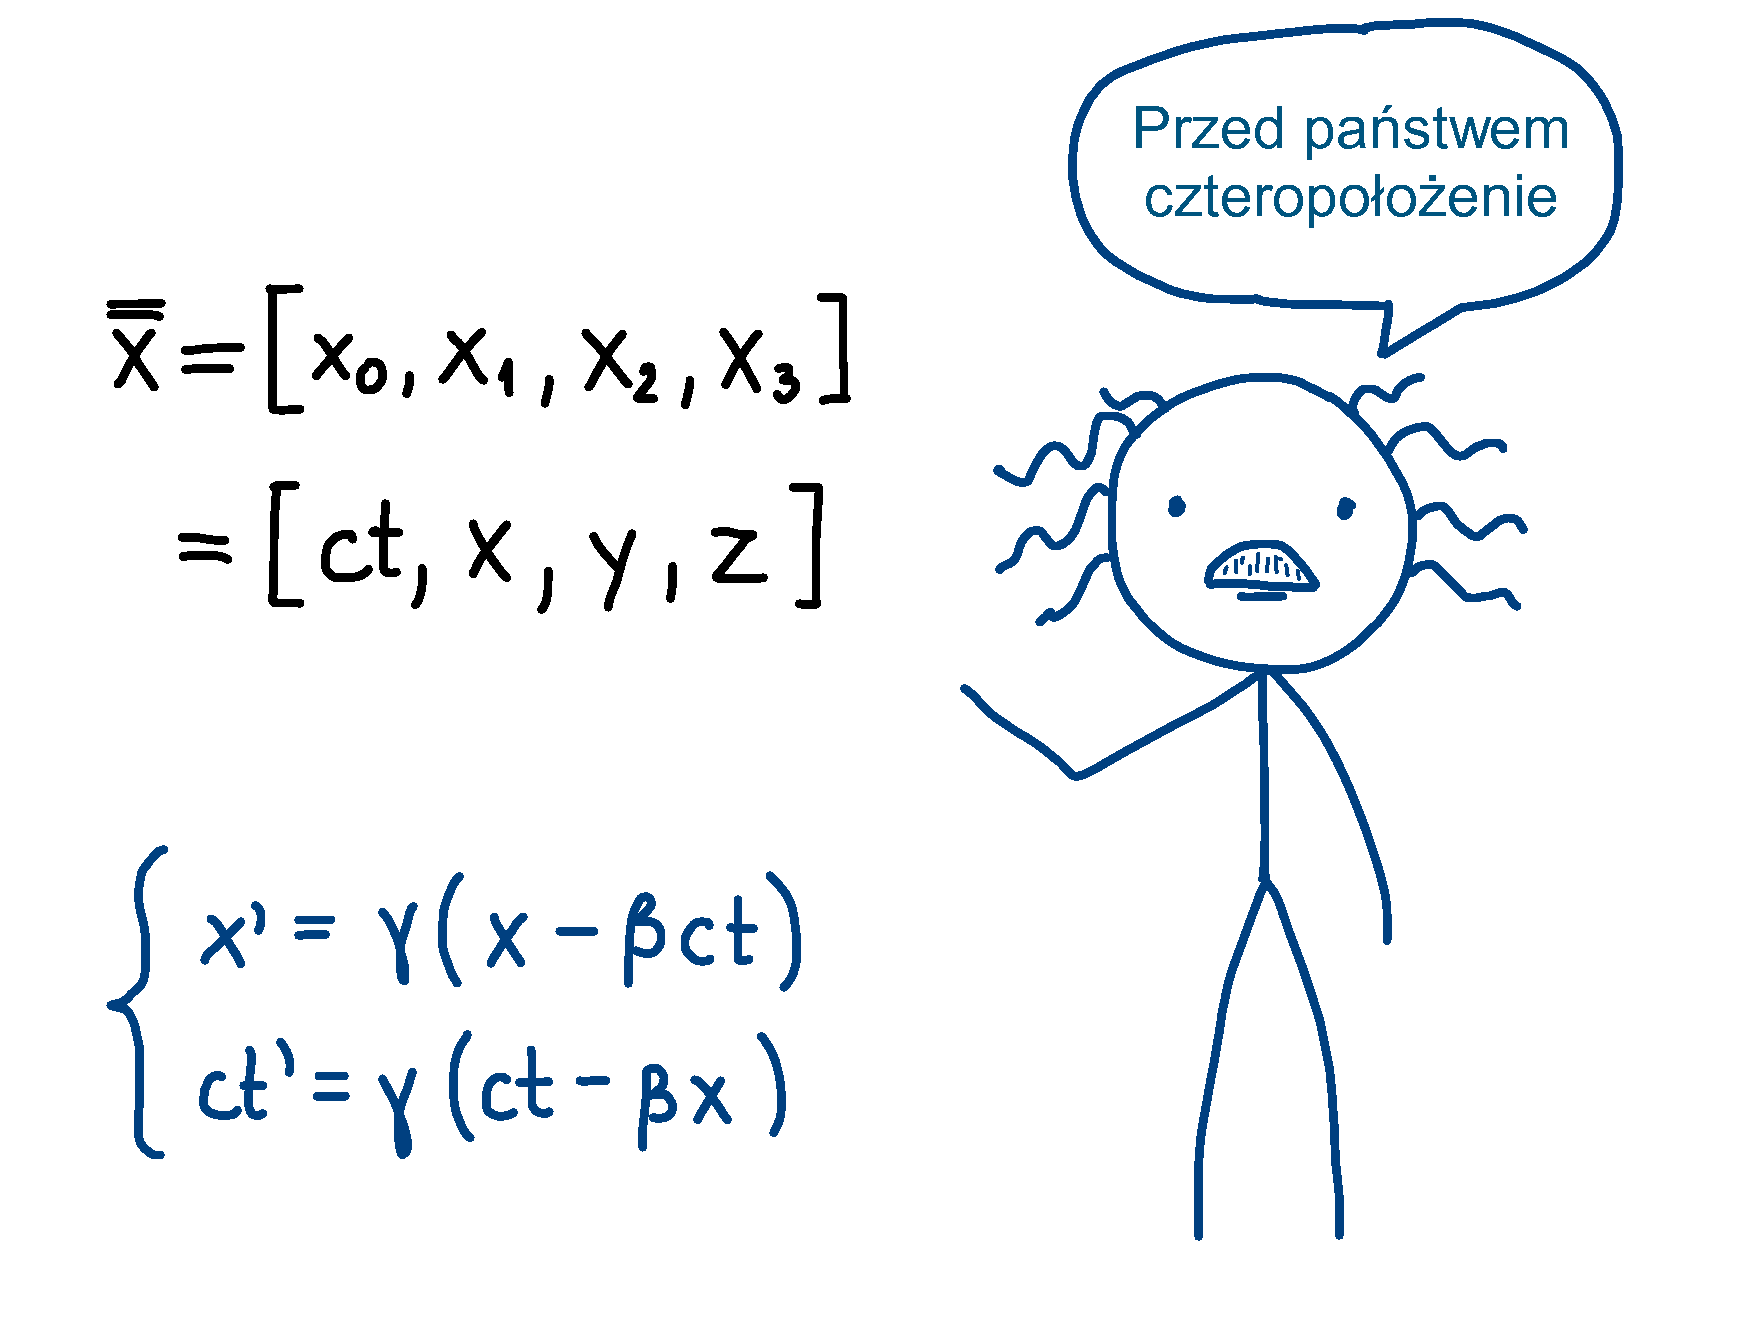
\includegraphics[width=1\linewidth]{pages/STA-page23}
Skoro przestrzeń i czas nie są już oddzielnymi, niezależnymi od siebie bytami,
a raczej współistniejącymi współrzędnymi, które przekształcają się razem,
możemy potraktować je jako jeden czteroelementowy wektor -- czterowektor\footnotemark.
\[
  \fourvec{x} = [x_0, x_1, x_2, x_3] = [ct, x, y, z] = [ct, \vec{r}]
\]

Czterowektor ma cztery współrzędne i wskazuje punkt w czterowymiarowej czasoprzestrzeni.
Różnica między tą przestrzenią (opisaną przez Hermanna Minkowskiego i nazwaną
przestrzenią Minkowskiego) a przestrzenią Euklidesową jest hiperboliczny obrót
gdy w grę wchodzi czas. Konsekwencją jest dość nietypowe wyrażenie na ``długość''
wektora
\[s^2 = (ct)^2 - (x^2 + y^2 + z^2),\]
co będzie miało fizycznie znaczenie później.

\footnotetext{Czterowektory oznaczam dwiema kreskami $\fourvec{x}$
  by podkreślić, kiedy mamy do czynienia z wektorem trój- a kiedy
  czterowymiarowym. Nie jest to konwencja, a czterowektory są po prostu wektorami.}
\newpage

\noindent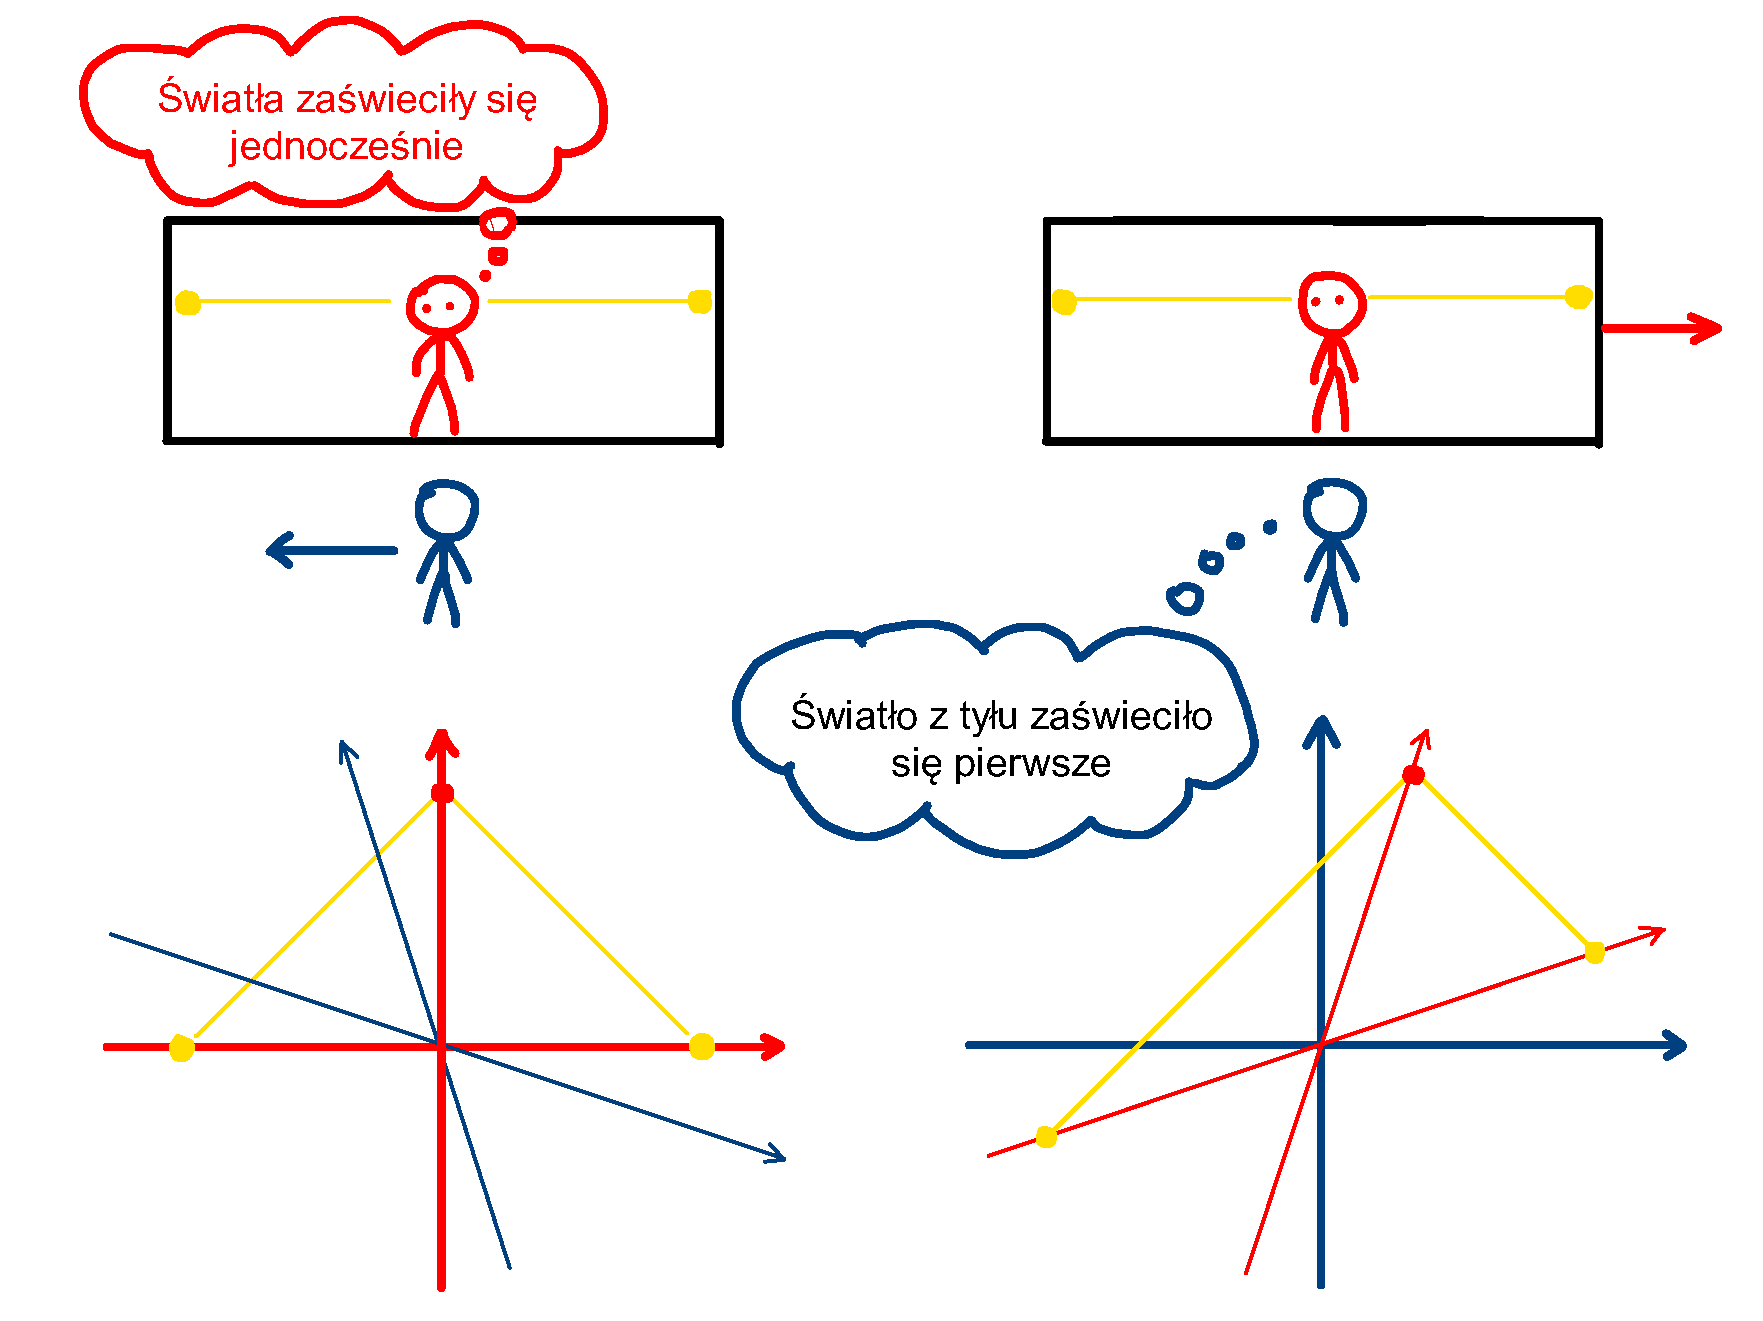
\includegraphics[width=1\linewidth]{pages/STA-page24}
Przetestujmy naszą nową teorię na przykładzie. Wykonamy nieco zmodyfikowaną
wersję eksperymentu myślowego zaproponowanego przez Alberta Einsteina.

Na środku wagonu subluminalnego ekspresu stoi Beata. Wagon ma długość \SI{2}{ls}
(sekundy świetlne) i na jego końcach znajdują się lampy ostrzegawcze, które
zapalają się, gdy wagon mija peron.
Wagon ma bardzo nowoczesny design i jest
cały oszklony tak, że można z zewnątrz obserwować, co się dzieje w środku.
Pociąg właśnie przejeżdżał z prędkością $u = 0.6c$ obok peronu, na którym stał Albert,
co Beacie zasygnalizowało jednoczesne zaświecenie się obu lamp ostrzegawczych.

Żeby uniknąć niejasności, Beata \textit{zobaczyła} obie lampy zapalające się w tym samym
czasie. Wiedząc, że stoi w równej odległości $d = \SI{1}{ls}$ od obu końców wagonu,
\textit{zmierzyła}, że lampy zaświeciły się jednocześnie sekundę wcześniej.
Podkreślam to, żeby pokazać, że efekty relatywistyczne nie są sztuczką wynikającą
z opóźnionego widzenia zjawisk, spowodowanym skończoną prędkością światła, a faktyczną
zmianą współrzędnych przestrzennych i czasowych zdarzeń niezależną od tego, kiedy
i gdzie zostają zobaczone. Każdy obserwator po \textit{zobaczeniu} zdarzenia,
może \textit{zmierzyć} gdzie w czasoprzestrzeni się ono zdarzyło.

Przejdźmy teraz do układu Alberta, który stoi na peronie. Ponieważ zarówno Albert
jak i Beata są inercjalni, obserwowane przez nich zjawiska powinny być identyczne.
Dla uproszczenia przesuńmy układ współrzędnych Alberta tak, aby jego punkt $(0, 0)$
pokrywał się z Beaty. Możemy to zrobić, ponieważ fizyka jest niezmienna przy przesunięciach.
Wykonajmy najpierw transformację Galileusza, żeby pokazać na czym polega problem
i jak rozwiązuje go transformacja Lorentza.

Jeśli czas byłby absolutny, to Albert również zobaczyłby, że oba światła zaświecają
się równocześnie. Według Beaty współrzędne zaświecenia się lamp wynoszą
\[
  \begin{bmatrix}\mred{t_1} \\ \mred{x_1}\end{bmatrix} =
  \begin{bmatrix} 0 \\ \SI{-1}{ls} \end{bmatrix};
  \begin{bmatrix}\mred{t_2} \\ \mred{x_2}\end{bmatrix} =
  \begin{bmatrix} 0 \\ \SI{1}{ls} \end{bmatrix}.
\]
Według Alberta będą one dokładnie takie same
\[
  \begin{bmatrix}\mblue{t_1'} \\ \mblue{x_1'}\end{bmatrix} =
  \begin{bmatrix} 0 \\ \SI{-1}{ls} \end{bmatrix};
  \begin{bmatrix}\mblue{t_2'} \\ \mblue{x_2'}\end{bmatrix} =
  \begin{bmatrix} 0 \\ \SI{1}{ls} \end{bmatrix}.
\]

Rozbieżność zaczyna się, gdy przeanalizujemy współrzędne zobaczenia świateł przez
Beatę. Według niej światło z obu lamp dotrze do niej dokładnie po sekundzie
\[
  \mred{t_{o1}} = \mred{t_{o2}} = \SI{1}{s}.
\]
Co zaś zmierzyłby Albert? Według niego Beata ucieka od światła wyemitowanego z tyłu wagonu
i zbliża się do światła wyemitowanego z przodu. Czas po którym tylne światło ją dogoni
wynosi zatem
\[ \mblue{t_{o1}} = \frac{d}{c - u} = \frac{\SI{1}{ls}}{0.4 c} = \SI{2.5}{s},\]
a czas dogonienia przedniego światła wynosi
\[ \mblue{t_{o2}} = \frac{d}{c + u} = \frac{\SI{1}{ls}}{1.6 c} = \SI{0.625}{s}.\]
Zatem, z jego punktu widzenia, do Beaty promienie światła nie dotarły jednocześnie.

Można by powiedzieć ``Wielkie rzeczy, przecież transformacja Lorentza też robi dziwne
rzeczy z przestrzenią i czasem. Dlaczego tamte dziwności mamy akceptować a tych nie?''
Miałoby to sens, gdyby nie to, że transformacja Galileusza powoduje
niemożliwe do zaistnienia sytuacje.

Co jeśli głowa Beaty eksploduje tylko wtedy,
gdy światła z obu lamp dotrą do niej jednocześnie? Inni pasażerowie jadący
z Beatą zobaczyliby jej mózg rozbryzgujący się na ścianach wagonu. Jednak według
ludzi na peronie Beata jedzie pociągiem dalej w jednym kawałku.
Gdyby teraz ktoś z peronu wsiadł do pociągu, mielibyśmy bardzo poważny problem
ustalić, co zastanie w środku. Według niego Beata żyje, ale inni w wagonie,
w tym sama Beata, by się z tym zdecydowanie nie zgodzili\footnote{Nie, to nie jest
  efekt kwantowy. Nie doszukuj się tu paradoksu Shr\"odingera.}.

Jak zatem z tym samym problemem poradzi sobie transformacja Lorentza?
Przy prędkości $u = 0.6 c$ współczynnik Lorentza wynosi $\gamma = 1.25$.
Zaczynamy w ten sam sposób, w układzie Beaty światła zaświecają się równocześnie
na obu końcach pociągu
\[
  \begin{bmatrix}\mred{ct_1} \\ \mred{x_1}\end{bmatrix} =
  \begin{bmatrix} 0 \\ \SI{-1}{ls} \end{bmatrix};
  \begin{bmatrix}\mred{ct_2} \\ \mred{x_2}\end{bmatrix} =
  \begin{bmatrix} 0 \\ \SI{1}{ls} \end{bmatrix}.
\]
Światło z obu lamp dociera do niej dokładnie po sekundzie powodując eksplozję
jej głowy w punkcie
\[
  \begin{bmatrix}\mred{ct_o} \\ \mred{x_o}\end{bmatrix} =
  \begin{bmatrix}\SI{1}{ls} \\ 0 \end{bmatrix}.
\]

Jakie współrzędne zdarzeń zmierzy zatem Albert? Ponieważ położenie i czas nie są
rozdzielne i muszą być traktowane razem, musimy obliczyć gdzie i kiedy według
niego zaświecą się światła ostrzegawcze.
Pamiętaj, że z perspektywy pociągu, peron porusza się z prędkością $\beta = -0.6$.
\[
  \begin{bmatrix}\mblue{ct_1'} \\ \mblue{x_1'}\end{bmatrix} =
  \gamma\begin{bmatrix}
    \mred{ct_1} + \beta \mred{x_1} \\
    \mred{x_1} + \beta \mred{ct_1}
  \end{bmatrix} =
  \begin{bmatrix}\SI{-0.75}{ls} \\ \SI{-1.25}{ls}\end{bmatrix},
\]
\[
  \begin{bmatrix}\mblue{ct_2'} \\ \mblue{x_2'}\end{bmatrix} =
  \gamma\begin{bmatrix}
    \mred{ct_2} + \beta \mred{x_2} \\
    \mred{x_2} + \beta \mred{ct_2}
  \end{bmatrix} =
  \begin{bmatrix}\SI{0.75}{ls} \\ \SI{1.25}{ls}\end{bmatrix}.
\]
Już na pierwszy rzut oka widać, że zdarzenia, które były jednoczesne w układzie
Beaty, wcale takie nie są w innych układach. Osoby stojące na peronie zmierzą,
że tylne światło zaświeciło się wcześniej, zaś przednie później.

Można teraz wyznaczyć gdzie i kiedy światło wyemitowane przez
lampy dotrze do Beaty. Najprościej zrobić to układając układ równań dla położenia
frontów fali świetlnych oraz położenia Beaty.
Otrzymamy z nich, że światła z obu lamp spotkają się z Beatą w tym samym czasie
w punkcie
\[ \begin{bmatrix}\mblue{ct_o} \\ \mblue{x_o}\end{bmatrix} =
  \begin{bmatrix}
    \SI{1.25}{ls} \\ \SI{0.75}{ls}
  \end{bmatrix}, \]
rozsadzając jej głowę.

Różni obserwatorzy może i nie są teraz zgodni gdzie i kiedy coś się zdarzyło,
ale dzięki temu są zgodni co się zdarzyło, a to dużo ważniejsze.
\newpage

\noindent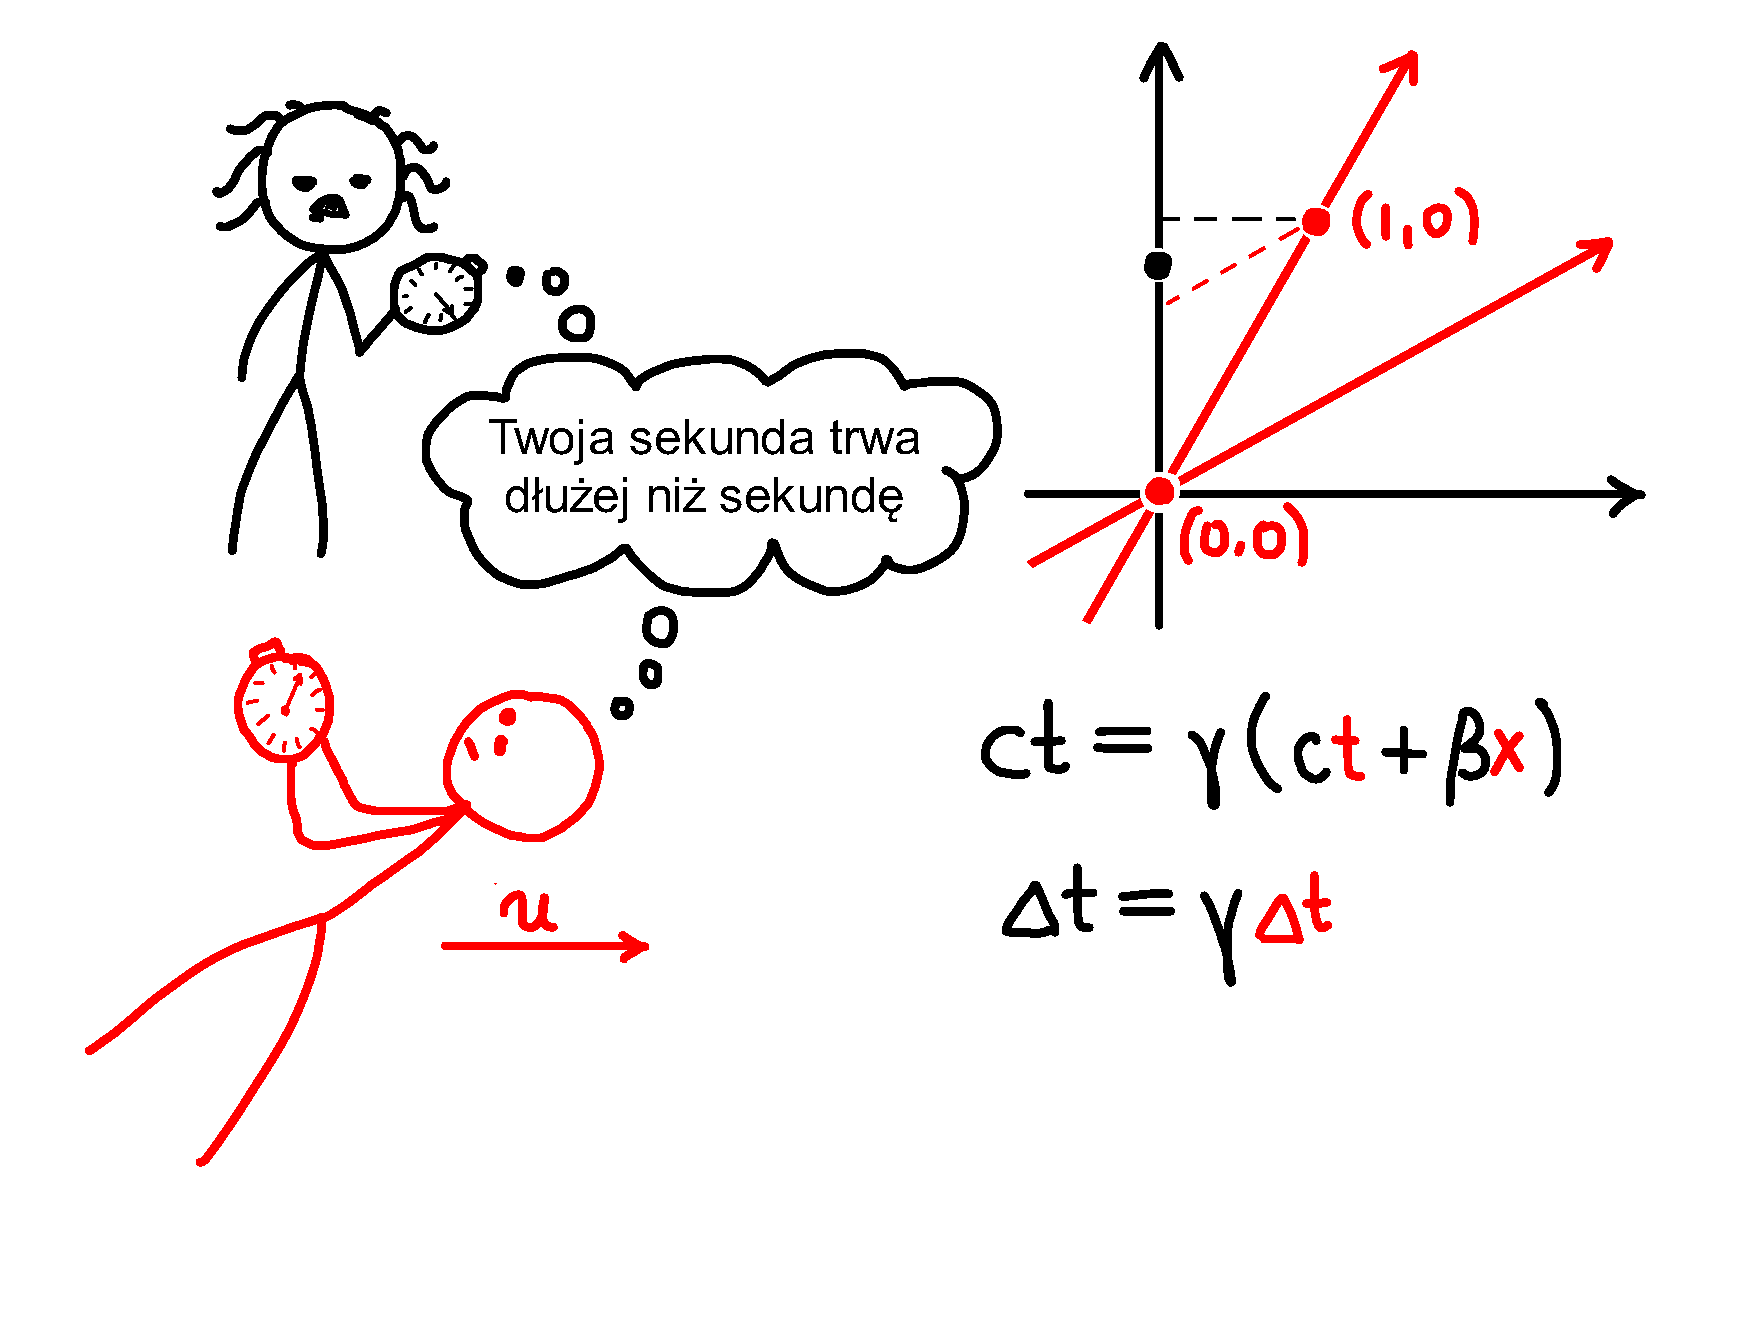
\includegraphics[width=1\linewidth]{pages/STA-page25}
Niejednoczesność jednoczesnych zdarzeń nie jest jedyną nietypową rzeczą,
z którą przyjdzie nam się zmierzyć. Wiele podręczników wprowadza w tym
momencie zjawisko \textit{dylatacji czasu}, opisując że czas obiektów będących w
ruchu upływa wolniej. Wynika to bezpośrednio z transformacji Lorentza.
Każda sekunda na kieszonkowym zegarku Beaty jest odmierzania, według niej,
w punkcie $\mred{x} = 0$. Podstawiając to do transformacji czasu w formie
różnicowej
\[c\mblue{\Delta t} = \gamma (c\mred{\Delta t'} + \beta \mred{\Delta x'}),\]
otrzymujemy
\[\mblue{\Delta t} = \gamma \mred{\Delta t'}.\]
Jeśli Beata przelatuje obok Alberta, to Albert zobaczy, że zmierzenie sekundy
przez zegarek Beaty będzie trwało $\gamma$ razy dłużej.

Ale chwila moment, przecież z punktu widzenia Beaty to Albert jest w ruchu
i to jego czas upływa wolniej
\[\mred{\Delta t'} = \gamma \mblue{\Delta t}.\]
Albert i Beata nie mogą być jednocześnie starsi i młodsi w
w stosunku do tego drugiego. Gdyby nasi bohaterowie się spotkali i
porównali swój wiek, to muszą być razem zgodni co do obserwacji.

Paradoks tkwi w tym, że czas jest tu wyjęty z szerszej perspektywy.
Jak ustaliliśmy wcześniej, współrzędne czasowe i przestrzenne nie są
rozdzielne i muszą być traktowane razem. Rozważanie samego czasu bez
przestrzeni sprowadzi nas na manowce.

Skorzystajmy jeszcze raz z transformacji Lotentza, tym razem w pełnej formie.
\[
  \begin{eqsystem}
    c\mblue{t} = \gamma (c\mred{t'} + \beta \mred{x'}) \\
    \mblue{x} = \gamma (\mred{x'} + \beta c\mred{t'})
  \end{eqsystem}.
\]
Kolejne sekundy Beaty będą mierzone przez nią samą w punktach
\[
  \mred{B_B} = \left\{
  \begin{bmatrix} 0 \\ 0 \end{bmatrix},
  \begin{bmatrix} 1 \\ 0 \end{bmatrix},
  \begin{bmatrix} 2 \\ 0 \end{bmatrix},
  \begin{bmatrix} 3 \\ 0 \end{bmatrix},
  \dots
  \right\}.
\]
Albert zaś zmierzy te same zdarzenia w punktach
\[
  \mblue{B_A} = \left\{
  \begin{bmatrix} 0 \\ 0 \end{bmatrix},
  \begin{bmatrix} \gamma \\ \gamma\beta \end{bmatrix},
  \begin{bmatrix} 2\gamma \\ 2\gamma\beta \end{bmatrix},
  \begin{bmatrix} 3\gamma \\ 3\gamma\beta \end{bmatrix},
  \dots
  \right\}.
\]
Analogicznie, Albert mierzy swoje sekundy w punktach
\[
  \mblue{A_A} = \left\{
  \begin{bmatrix} 0 \\ 0 \end{bmatrix},
  \begin{bmatrix} 1 \\ 0 \end{bmatrix},
  \begin{bmatrix} 2 \\ 0 \end{bmatrix},
  \begin{bmatrix} 3 \\ 0 \end{bmatrix},
  \dots
  \right\},
\]
a Beata zmierzy je w punktach
\[
  \mred{A_B} = \left\{
  \begin{bmatrix} 0 \\ 0 \end{bmatrix},
  \begin{bmatrix} \gamma \\ -\gamma\beta \end{bmatrix},
  \begin{bmatrix} 2\gamma \\ -2\gamma\beta \end{bmatrix},
  \begin{bmatrix} 3\gamma \\ -3\gamma\beta \end{bmatrix},
  \dots
  \right\}.
\]

Albert faktycznie zaobserwuje, że każda sekunda Beaty jest odmierzona przez nią
w odstępach większych niz sekunda i vice-versa, ale są też odmierzane
coraz dalej od niego. Kluczowe jest też to, że poruszając się ruchem jednostajnym
nigdy nie będą mieli okazji spotkać się ponownie by porównać czas z bliska.
Dylatacja czasu jest nierozerwalnie połączona ze zmienianiem położenia.

Jeśli jesteś zainteresowany zgłębieniem tematu, to po przerobieniu całego
wykładu spróbuj policzyć upływ czasu w sytuacji, gdy Beata zwalnia i zawraca
by znów spotkać Alberta. Można to wyznaczyć całkując po czasie własnym lub
licząc długość zakrzywionej linii świata w czasoprzestrzeni Minkowskiego.
Wtedy okazuje się, że od ostatniego spotkania upłynęło jej mniej lat niz Albertowi.
Receptą na podróż do przyszłości jest szybka podróż w tą i z powrotem
(albo czekanie na kanapie aż przyszłość przyjdzie do nas sama).
\newpage

\noindent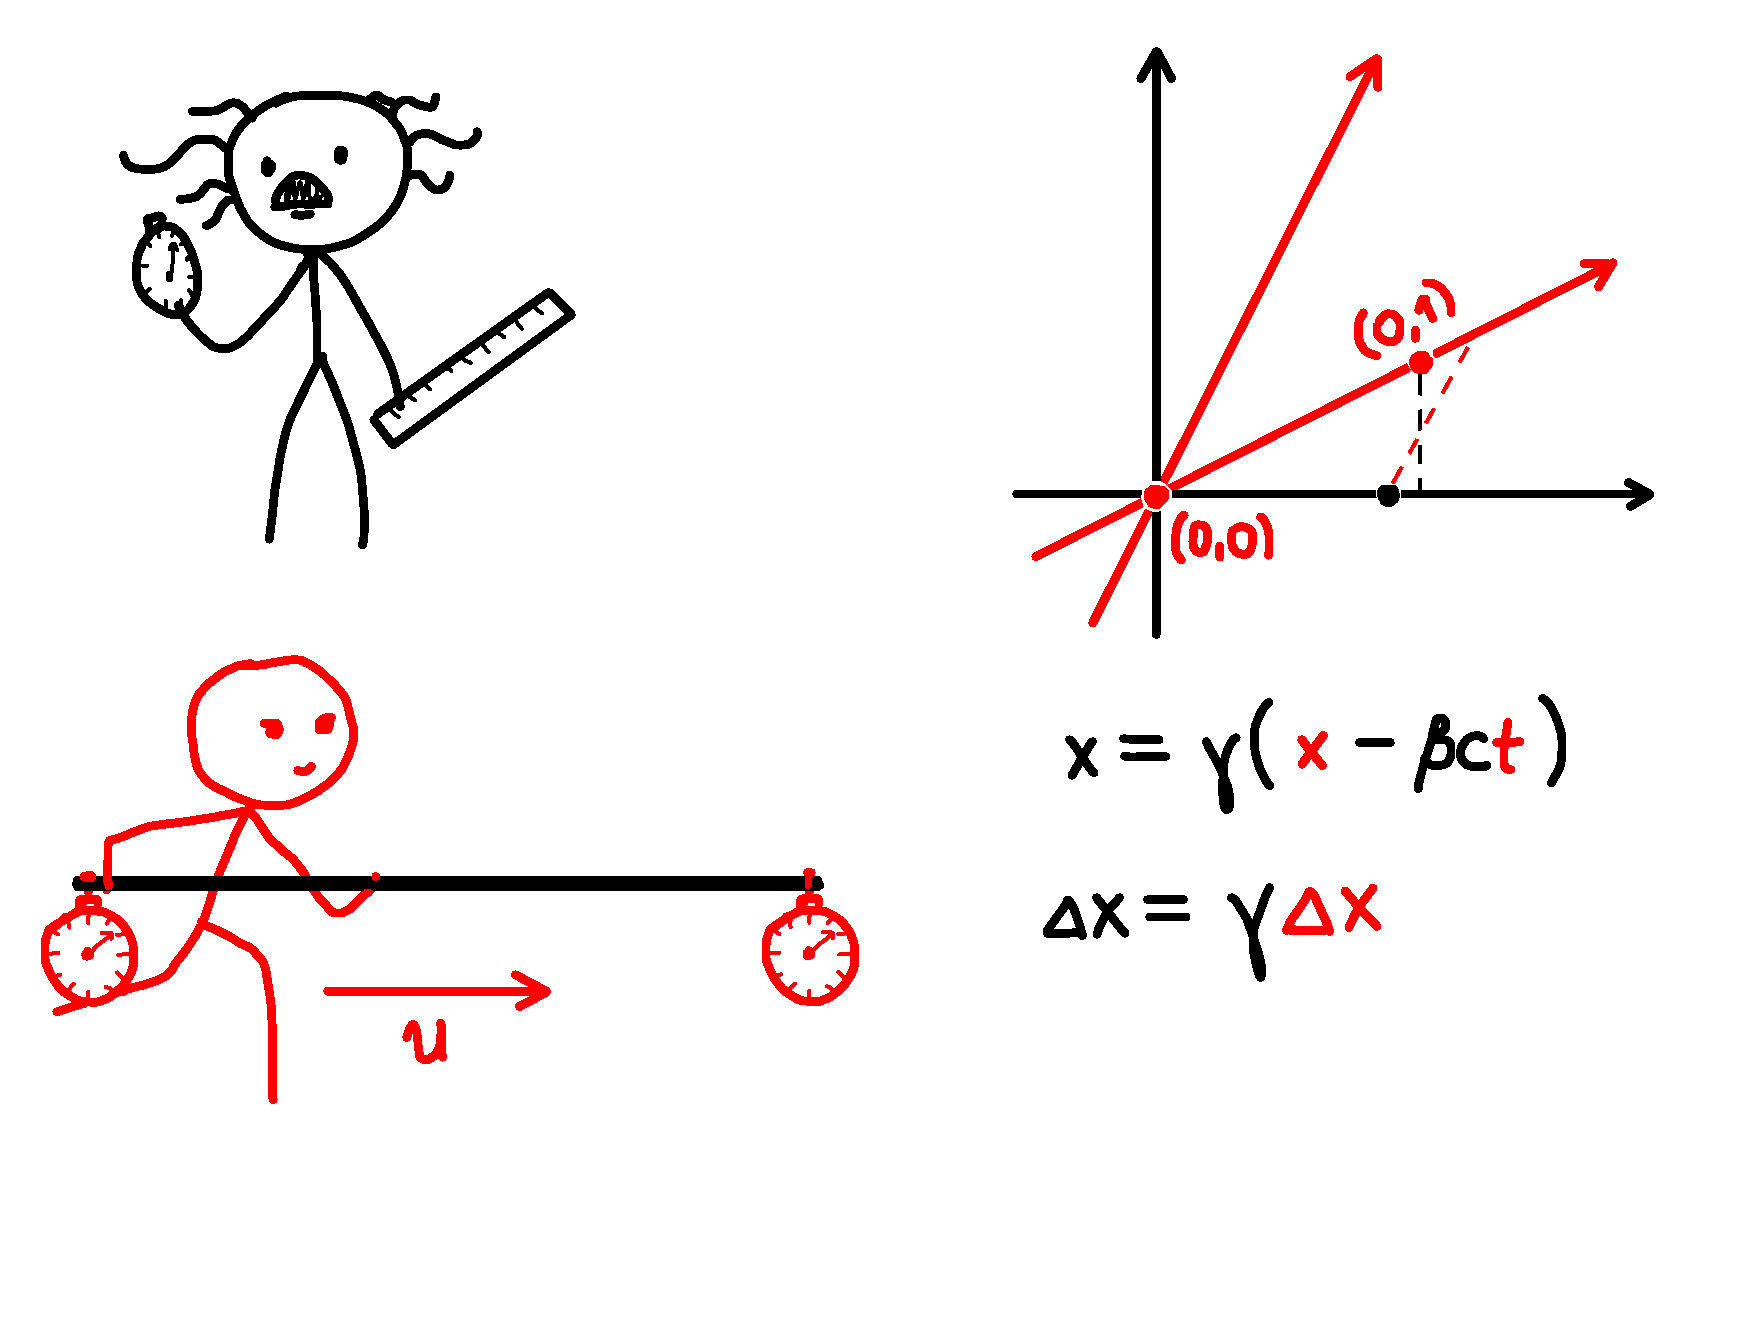
\includegraphics[width=1\linewidth]{pages/STA-page26}
Skomplikujmy teraz nieco sprawę. Ustaliliśmy, że Albert i Beata mogą jednocześnie
obserwować, że to drugie jest młodsze. Tak długo jak poruszają się ruchem
jednostajnym i mają tylko jedną szansę spotkać się z bliska, żeby porównać
swój wiek, nie prowadzi to do paradoksu.

Co jeśli Beata będzie trzymać w rękach bardzo długi kij, do którego z przodu
i z tyłu przymocuje zsynchronizowane zegarki odmierzające jej wiek?
Ten kij może być nawet nieskończenie długi i mieć w regularnych odstępach przymocowane
zsynchronizowane zegary, tak, żeby Albert w każdej chwili mógł
sprawdzić ile lat ma Beata bez spotykania jej po raz drugi.
Nie ma teraz innej opcji, zegarek Alberta musi wskazywać czas
wcześniejszy, albo późniejszy niż mijany przez niego zegar Beaty.

Czy ten sposób będziemy mogli absolutnie ustalić, które z nich jest
młodsze? Nie! Zarówno Albert jak i Beata zmierzą, że każdy mijany przez niego zegar
na kiju wskazuje \textbf{dokładnie} ten sam czas co jego własny.
Jak to możliwe skoro mamy dylatację czasu a zegary pokazują aktualny
wiek Beaty? Otóż nie pokazują! Tak samo jak w eksperymencie z wagonem,
zdarzenia jednoczesne dla jednego, nie będą jednoczesne dla drugiego.
Zegary zsynchronizowane przez Beatę nie będą
zsynchronizowane w układzie odniesienia Alberta.
Według niego wszystkie chodzą wolniej o czynnik $\gamma$,
ale te z tyłu kija pokazują późniejszą godzinę -- zostały wystartowane wcześniej.
W ten sposób, każdy zegar w chwili mijania będzie pokazywać dokładnie tą samą godzinę co jego własny.
Pomimo bycia bardzo nieintuicyjną na chłopski rozum, STW zapewnia nam
spójne obserwacje.

Sugeruję ci w tym momencie samodzielnie przeliczyć sytuację, w której Beata biegnie
z kijem, to którego na obu końcach przymocowane są budziki.
Jeśli oba budziki zadzwonią w tej samej chwili według Beaty, to w jakich
miejscach i czasie zadzwonią według Alberta?

Jako dodatek wyobraźmy sobie, że subluminalny pociąg jest cały wypełniony
Beatami w ``tym samym'' wieku.
Stojący na peronie Albert widziałby, że jadące Beaty siedzące z
tyłu pociągu są starsze od tych z przodu.
\newpage

\noindent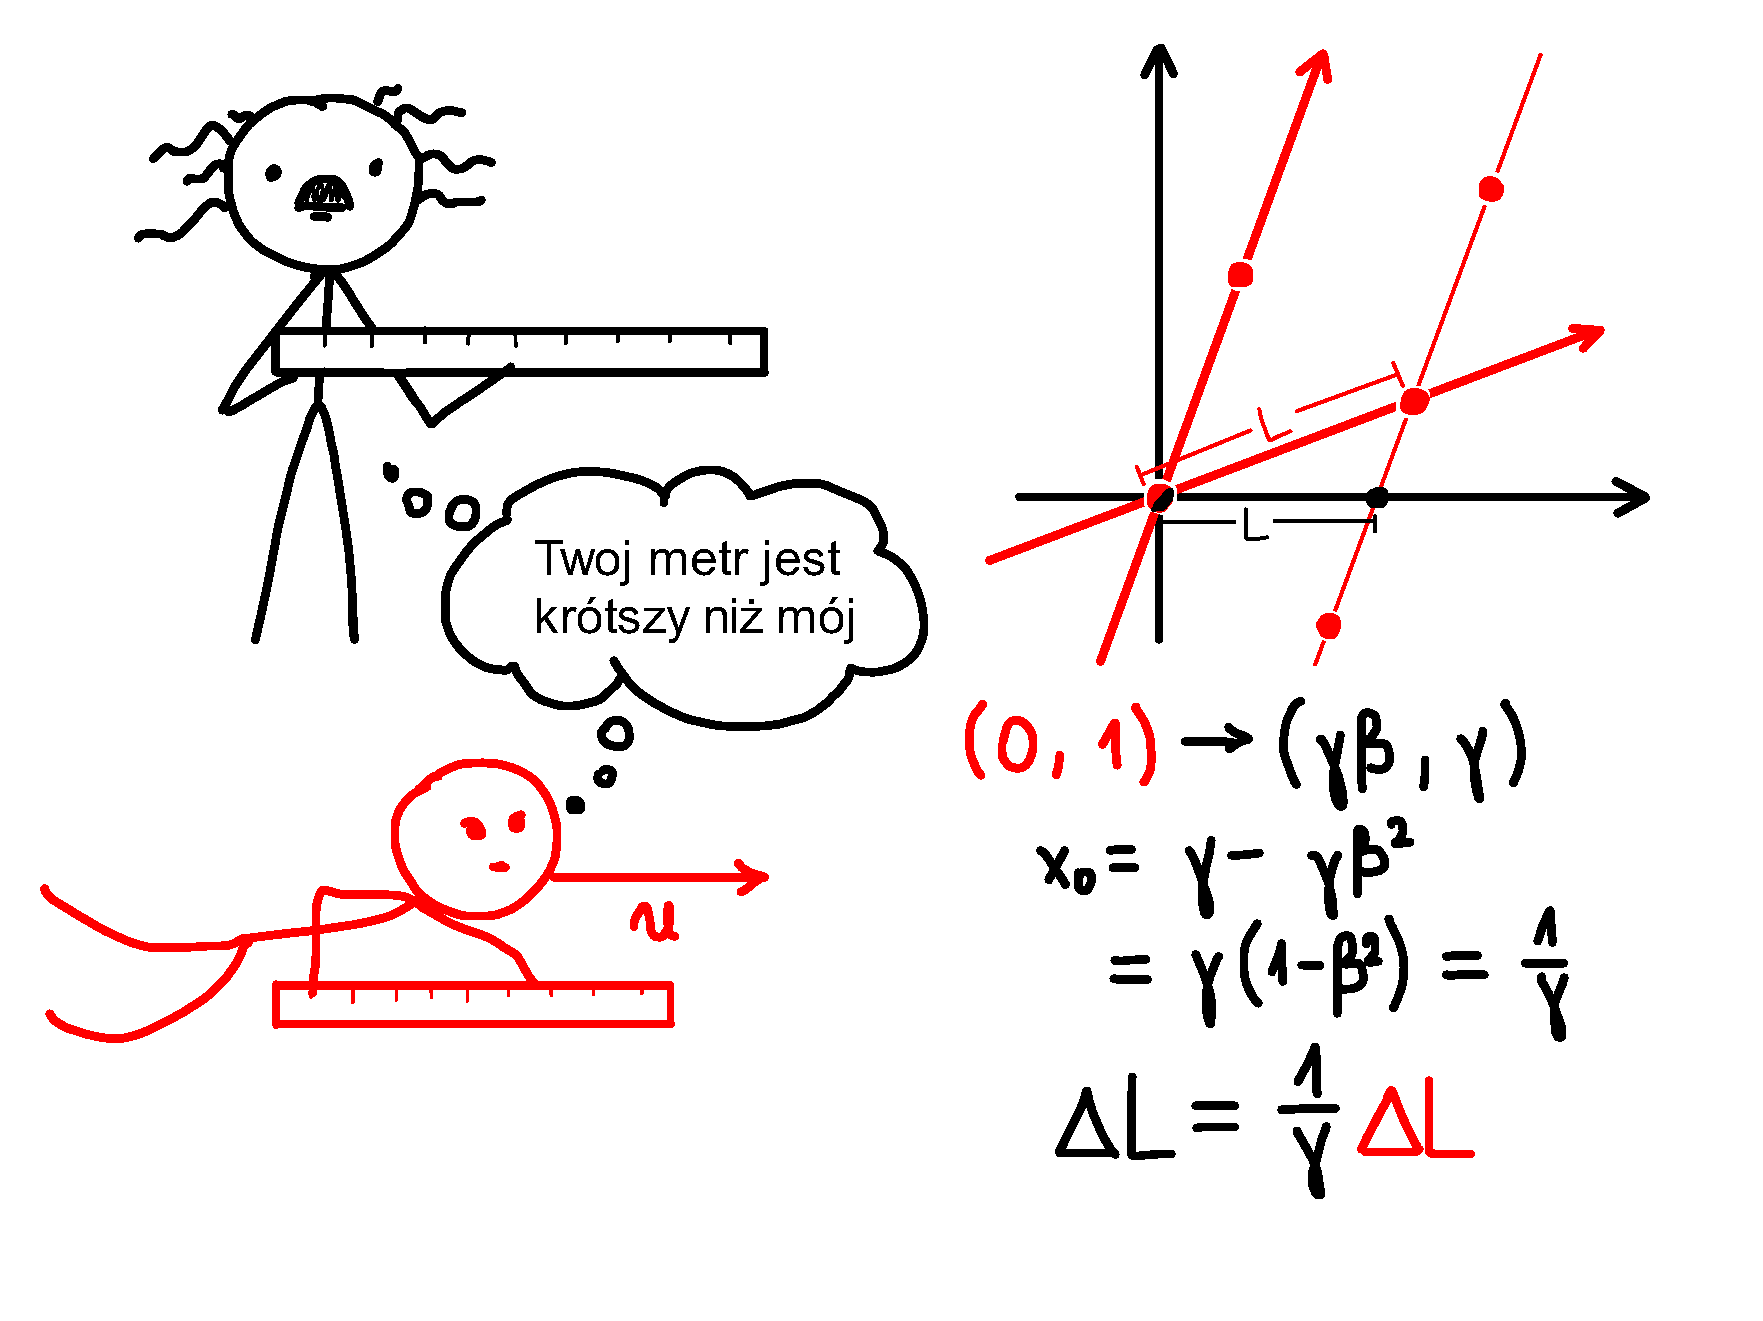
\includegraphics[width=1\linewidth]{pages/STA-page27}
W ten sam sposób co policzyliśmy dylatacje czasu oddzielającego od siebie zdarzenia,
możemy też policzyć zmianę odległości między zdarzeniami. Podstawiamy wtedy
$\Delta t = 0$ w równaniu transformacji $\Delta x$ i otrzymamy
\[ \mblue{\Delta x} = \gamma \mred{\Delta x'}. \]

Chwila moment. Przecież Lorentz zaproponował, że obiekty będą się skracać w kierunku ruchu
a samo zjawisko nosi nazwę \textit{skrócenia} Lorentza.
Tutaj zdecydowanie mamy wydłużenie.

Owszem! To dlatego, że to wcale nie jest długość tylko odległość między dwoma zdarzeniami.
Długość to nic innego jak jednoczesne zmierzenie położenia początku i końca.
A gdzie coś jest \textit{jednoczesne} tam są problemy.

Zróbmy jak zawsze eksperyment myślowy. Beata jednocześnie mierzy położenia początku
i końca metrowej linijki. Dla niej oczywiście $\mred{\Delta t} = 0$ i $\mred{\Delta x} = L$.
Zaś według Alberta $\mblue{\Delta x'} = \gamma L$ ale również $\mblue{\Delta t'} = \gamma\beta L$.
Dla niego, Beata zmierzyła położenie tylnego końca linijki przed przednim (licząc względem kierunku ruchu).
Taki pomiar odległości nie ma dla Alberta sensu, bo linijka się w międzyczasie przemieściła!
To tak jakby mierzyć długość samochodu mierząc tył gdy ten wjeżdża do tunelu
i przód gdy wyjeżdża i dojść do wniosku, że samochód jest długości tunelu.
Kompletna bzdura!

Zróbmy zatem poprawkę i odejmijmy od odległości między zdarzeniami dystans,
który przebyła linijka w tym czasie.
\[
  \mblue{L'} = \gamma L - \gamma \beta L \beta = \gamma L (1 - \beta^2) = L \frac{1 - \beta^2}{\sqrt{1 - \beta^2}} = L \sqrt{1 - \beta^2} = \frac{L}{\gamma}
\]
To zdecydowanie jest skróceniem i to tym samym, które pierwotnie zaproponował Lorentz
by wyjaśnić wynik eksperymentu Michelsona-Morleya.
\newpage

\noindent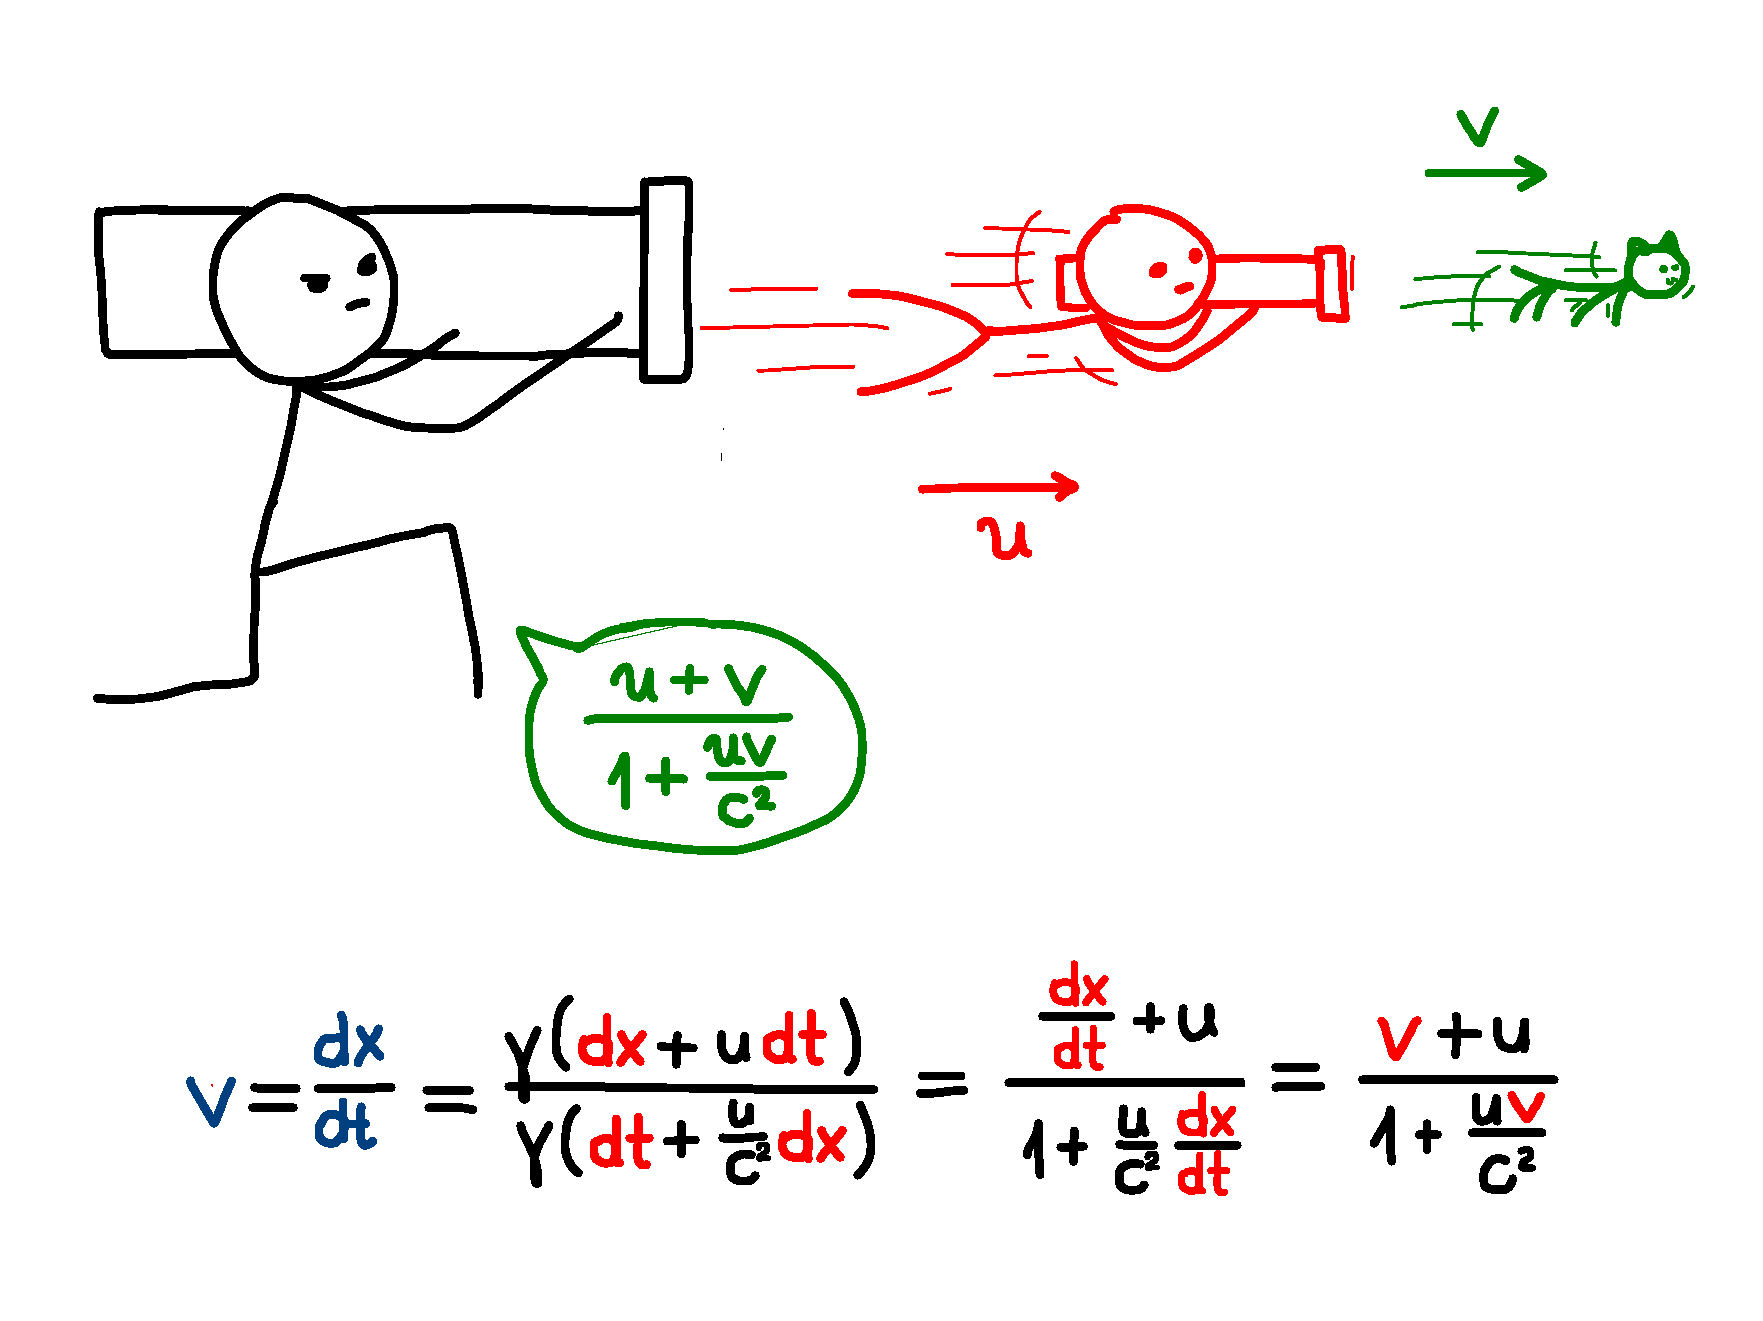
\includegraphics[width=1\linewidth]{pages/STA-page28}
Sprawdźmy jeszcze jak w czasoprzestrzeni składają się prędkości.
Tradycyjna suma prędkości stosowana przez Galileusza i Newtona nie daje
prawidłowych wyników, ale wiemy przecież, że prędkości jakoś się dodają.

Użyjmy za przykład Alberta, wystrzeliwuje Beatę z wyrzutni z prędkością $u$,
która z kolei wystrzeliwuje z tym samym kierunku kota z prędkością $v$ (nie róbcie tego w domu).
Jaką prędkość kota zaobserwuje zatem Albert?

Najłatwiej ten problem policzyć używając transformacji Lorentza w formie różniczkowej
\[
  \begin{eqsystem}
    \mblue{\diff t} = \gamma (\mred{\diff t'} + \frac{u}{c^2}\mred{\diff x'}) \\
    \mblue{\diff x} = \gamma (\mred{\diff x'} + u \mred{\diff t'})
  \end{eqsystem},
\]
\[
  \mblue{v}
  = \mblue{\derivative[x]{t}}
  = \frac{\gamma (\mred{\diff x} + u \mred{\diff t})}{\gamma (\mred{\diff t} + \frac{u}{c^2} \mred{\diff x})}
  = \frac{\mred{\derivative[x]{t}} + u \mred{\derivative[t]{t}}}{\mred{\derivative[t]{t}} + \frac{u}{c^2}\mred{\derivative[x]{t}}}
  = \frac{\mred v + u}{1 + \frac{u \mred v}{c^2}}.
\]
Sprawdź teraz, że jeśli coś porusza się z prędkością światła w jednym układzie,
to porusza się też tak w każdym innym. Równocześnie, jeśli coś porusza się wolniej od
prędkości światła to też porusza się wolniej w każdym innym układzie.
\newpage

\noindent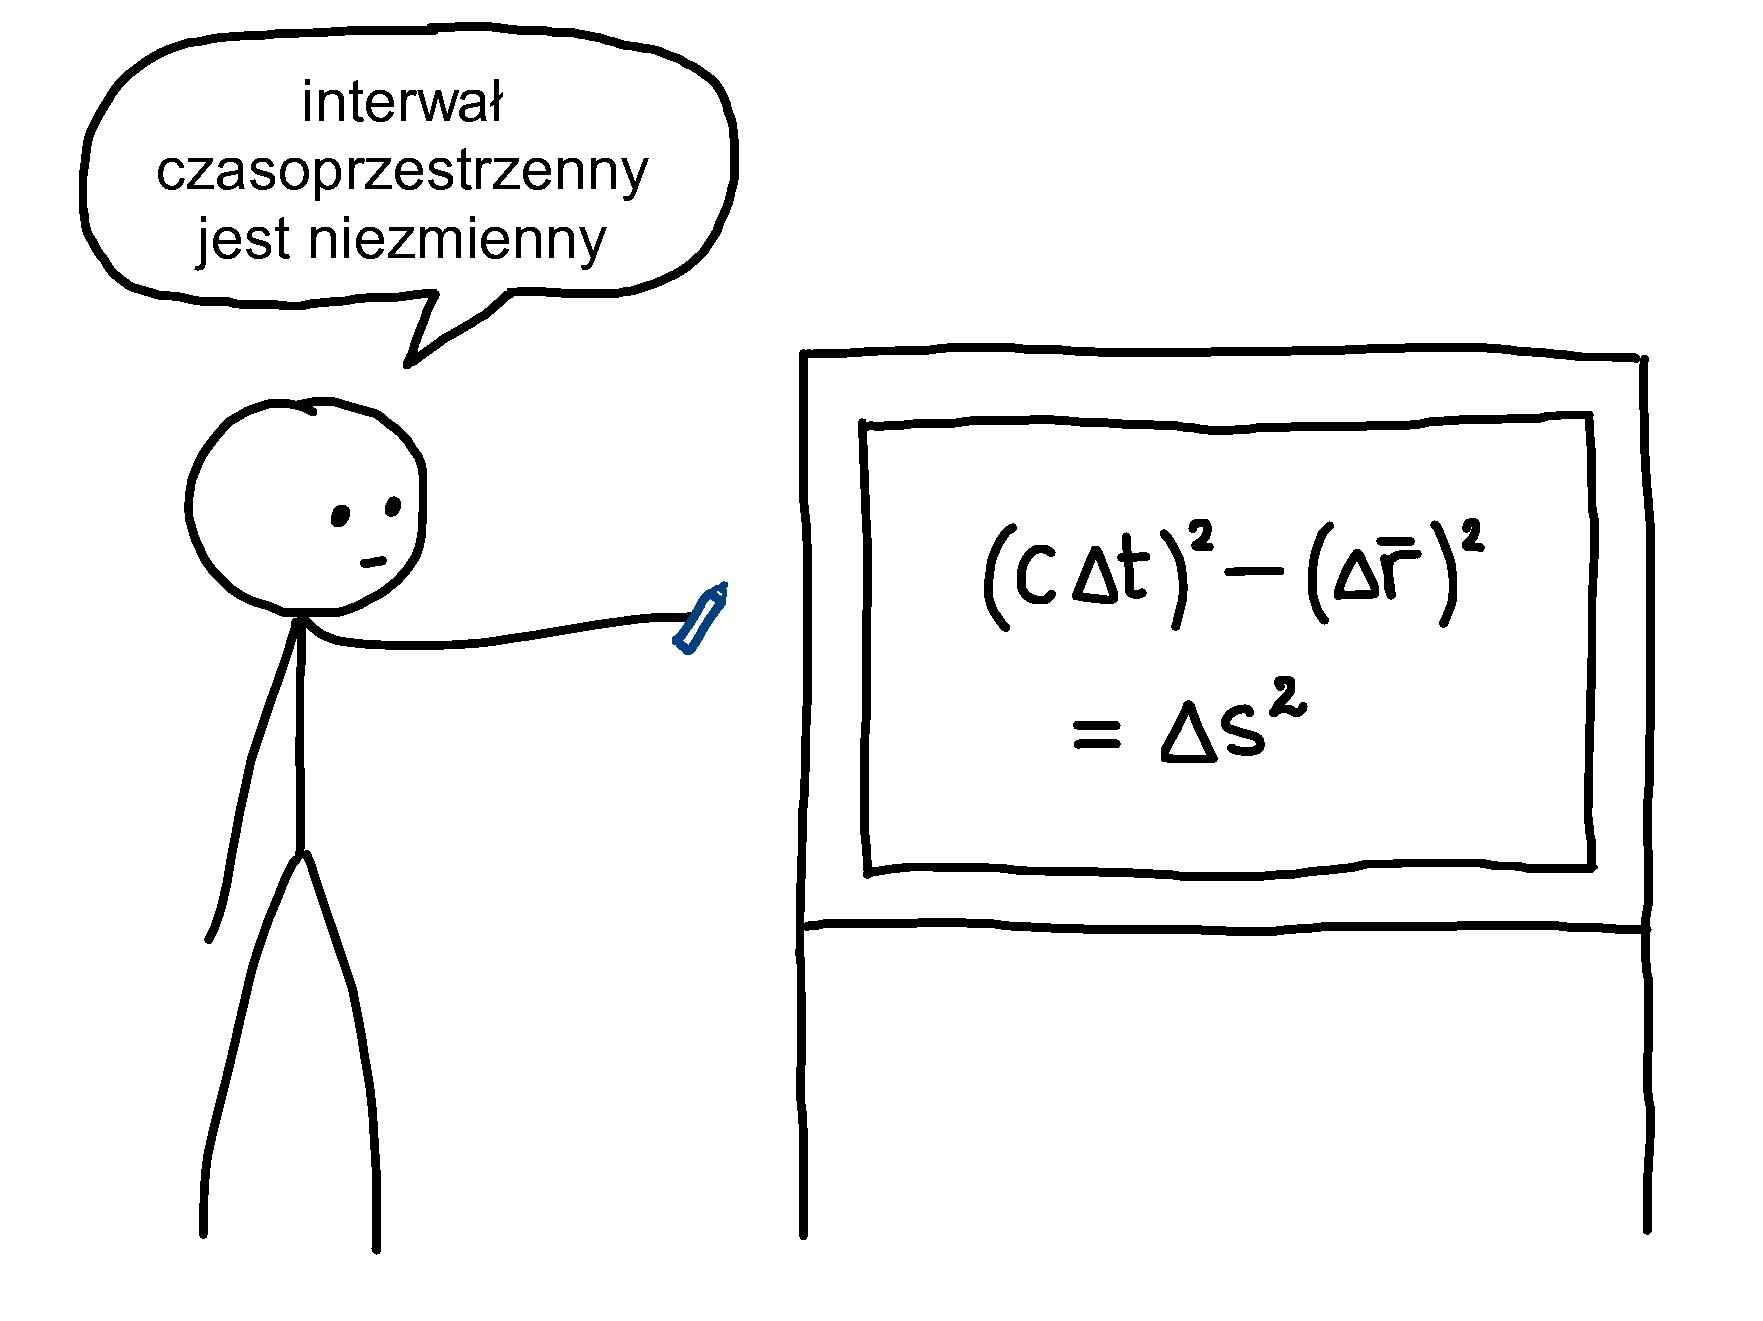
\includegraphics[width=1\linewidth]{pages/STA-page30}
Wróćmy do czegoś co do tej pory tylko napomknęliśmy, a co jest bardzo
istotnym elementem STW; czegoś co, w całej tej relatywności, pozostaje
absolutne. Podobnie jak w przestrzeni Galileusza odległości były niezmienne
tak i w czasoprzestrzeni Minkowskiego możemy zdefiniować ``długość'', która
będzie stała i niezależna od układu odniesienia. Musi ona jednak zawierać
w sobie komponent czasu. Ponieważ obrót hiperboliczny, którym matematycznie
jest transformacja Lorentza, nie zmienia równania hiperboli $x^2 - y^2 = a^2$
możemy użyć tego jako nowej definicji długości
\[
  (c \Delta t)^2 - \Delta x^2 = \Delta s^2.
\]
Wartość $\Delta s^2$, nazywana interwałem czasoprzestrzennym, określa
niezależną od obserwatora odległość między dwoma zdarzeniami w czasoprzestrzeni.

W czterech wymiarach, można go zapisać jako
\[
  \Delta s^2 = (c \Delta t)^2 - (\Delta x^2 + \Delta y^2 + \Delta z^2)
  = (c \Delta t)^2 - (\Delta \vec{r})^2.
\]
Jest to przydatne narzędzie, przy pomocy którego można policzyć niektóre
rzeczy bez uciekania się do pełnej transformacji Lorentza.
\newpage

\noindent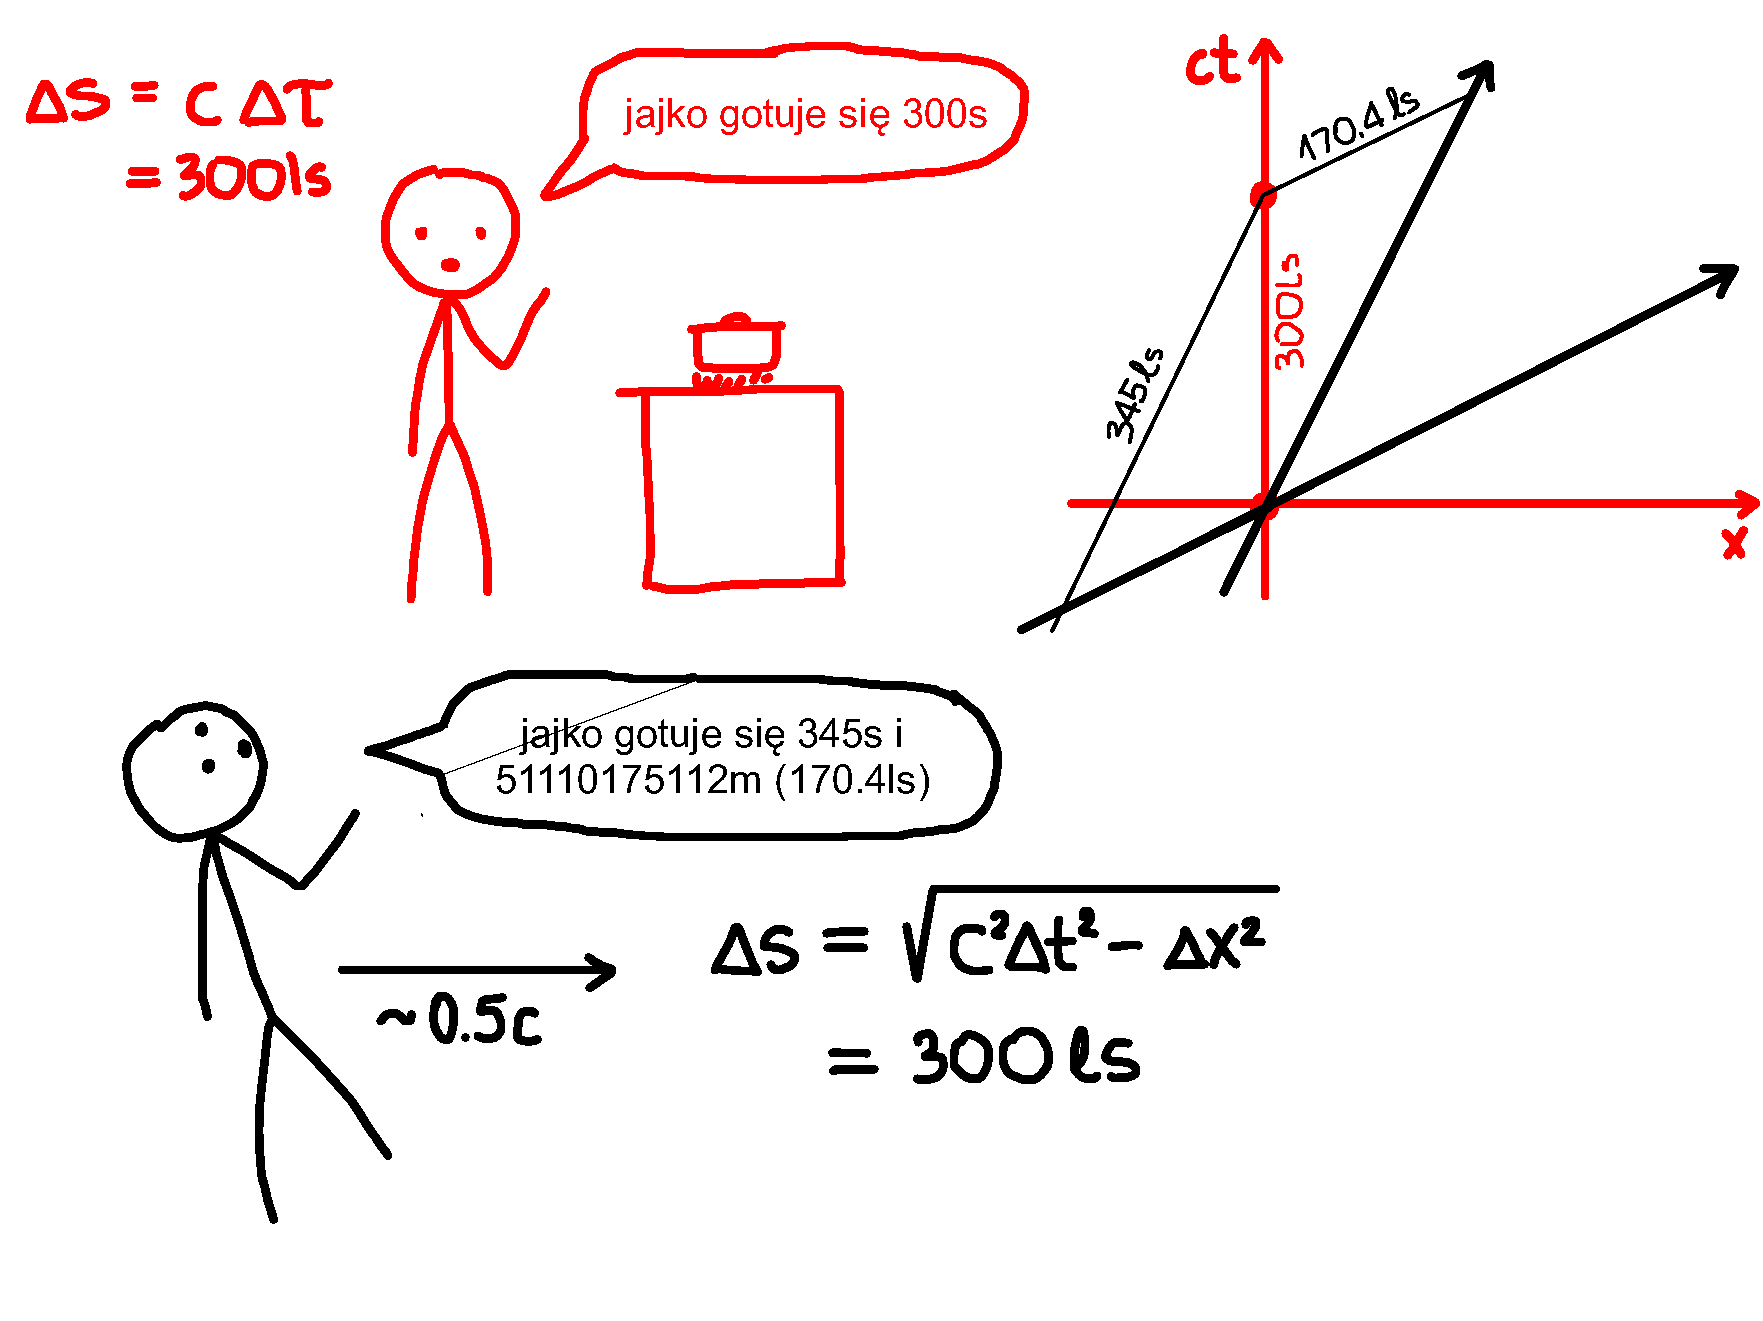
\includegraphics[width=1\linewidth]{pages/STA-page31}
Przetestujmy to i sprawdźmy ile czasu gotuje się jajko?
W przedziale restauracyjnym promu kosmicznego Beata rozpoczęła
gotowanie jajka na twardo. Dla prostoty, będzie to początek układu
współrzędnych. Jeśli jajko skończyło się gotować po \SI{300}{\second} i nigdzie
się w międzyczasie nie przemieściło ($\Delta x = 0$), to interwał między początkiem a
końcem gotowania wynosi
\[
  \Delta s^2 = (c\Delta t)^2 - \Delta x^2 = (\SI{300}{ls})^2.
\]
Dla Alberta, przelatującego obok z prędkością około $0.495c$, jajko gotuje się przez
\SI{345}{\second} ale również przemieszcza się w tym czasie o \SI{170.4}{ls}.
Dla niego, interwał między zdarzeniami rozpoczęcia i końca gotowania wynosi
\[
  \Delta s^2 = (c\Delta t)^2 - \Delta x^2 \approx (\SI{345}{ls})^2 - (\SI{170.4}{ls})^2 \approx (\SI{300}{ls})^2,
\]
czyli tyle samo.

Interwał czasoprzestrzenny ma jeszcze jedno ważne zastosowanie w fizyce. Zauważ, że w układzie,
w którym zdarzenia się dzieją (są w tym samym miejscu) interwał jest równy czasowi, który
upłynął między nimi $\Delta s^2 = c\Delta t^2$.

Jest to tak zwany czas własny oznaczany literą $\tau$ i jest to
też najkrótszy obserwowalny czas między zdarzeniami (w każdym innym układzie będzie dłuższy).
Mamy więc, że
\[
  (c\Delta \tau) ^2 = (c\Delta t)^2 - (\Delta \vec{r})^2.
\]
Możemy dzięki temu policzyć czas własny życia i rozpadu egzotycznych cząstek
formujących się w górnych warstwach atmosfery i akceleratorach, a także czas upływający
na satelitach GPS pędzących po orbicie okołoziemskiej.

Interwał w którym odległość w czasie jest większa od odległości w
przestrzeni, $\Delta s^2 > 0$, nazywamy interwałem czasowym. Jest nim na przykład
początek i koniec gotowania jajka. Z takimi dwoma zdarzeniami można powiązać czas własny
i występuje między nimi ścisłe następstwo czasowe. Żadnej inny obserwator nie zaobserwuje, że jajko
ugotowało się przed włączeniem gazu na kuchence.

Istnieje jednak drugi przypadek, w którym interwał czasoprzestrzenny jest ujemny.
W końcu nic nie stoi na przeszkodzie, żeby dwa zdarzenia wydarzyły się bardzo daleko od
siebie w krótkim odstępie czasu.
Mimo, że $\Delta s^2 < 0$ nie ma rzeczywistej wartości, taki przypadek jest dla nas
równie użyteczny i jest nazywany interwałem przestrzennym, bo dominuje
w nim odległość przestrzenna.
Niektórzy w takiej sytuacji odwracają znak interwału
\[\Delta \sigma^2 = -\Delta s^2 = (\Delta \vec r)^2 - (c\Delta t)^2.\]

Zauważ, że jeśli interwał jest ujemny,
to istnieje taki układ odniesienia, w którym czas między zdarzeniami wynosi $\Delta t = 0$,
a odległość między nimi jest wtedy najmniejsza. Analogicznie, ta długość jest nazwana
długością (odległością) własną.
Ponieważ istnieje układ odniesienia, w którym te dwa zdarzenia
zaszły jednocześnie, lub w całkiem odwrotnej kolejności,
to znaczy, że nie mógł łączyć ich ciąg przyczynowo-skutkowy.
Nie mają czasu własnego.

Przykładem są dwie lampy na końcach wagonu z poprzedniego eksperymentu.
Zaświecenie się jednej nie może wpłynąć na zaświecenie drugiej.
Różni obserwatorzy nie zgadzaliby się nawet co do kolejności tych dwóch zdarzeń.
Lampy mogą jednak mieć wspólną przyczynę w przeszłości.
\newpage

\noindent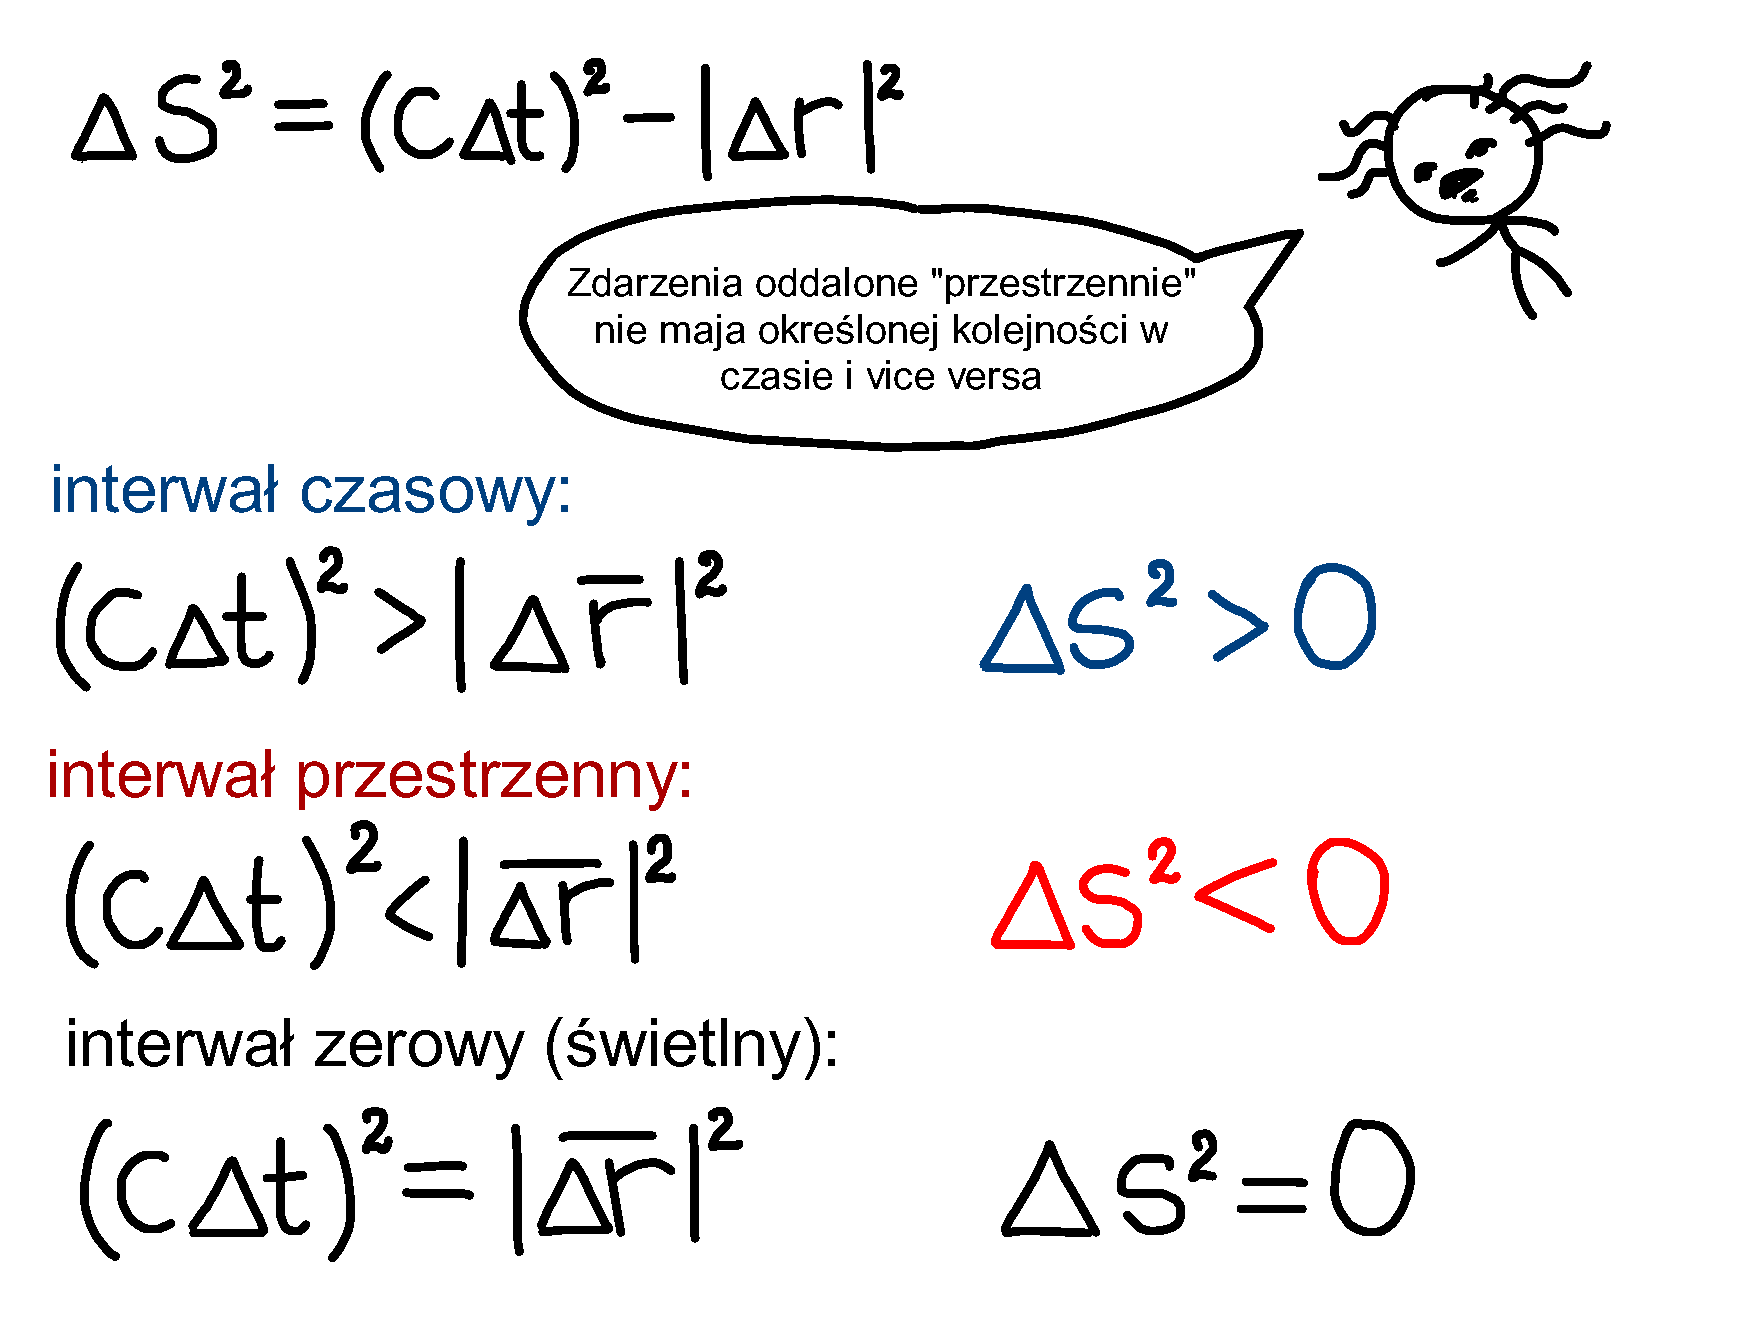
\includegraphics[width=1\linewidth]{pages/STA-page32}
Bazując na znaku, interwały można podzielić na trzy grupy
\begin{itemize}
  \item Interwał czasowy, gdy $\Delta s^2 > 0$.
        Łączy zdarzenia miedzy którymi występuje następstwo czasowe / przyczynowo-skutkowe.
        Można z nimi powiązać układ odniesienia i czas własny $c\Delta \tau = \pm\Delta s$.
  \item Interwał przestrzenny, gdy $\Delta s^2 < 0$.
        Łączy zdarzenia oddalone przestrzennie, których nie może łączyć ciąg przyczynowo-skutkowy.
        Istnieje układ odniesienia, w którym występują jednocześnie.
  \item Interwał zerowy, gdy $\Delta s^2 = 0$. Zarezerwowany dla zdarzeń gdzie
        $\frac{\Delta x}{\Delta t} = c$, na przykład kolejne położenia fali
        elektromagnetycznej.
\end{itemize}
\newpage

\noindent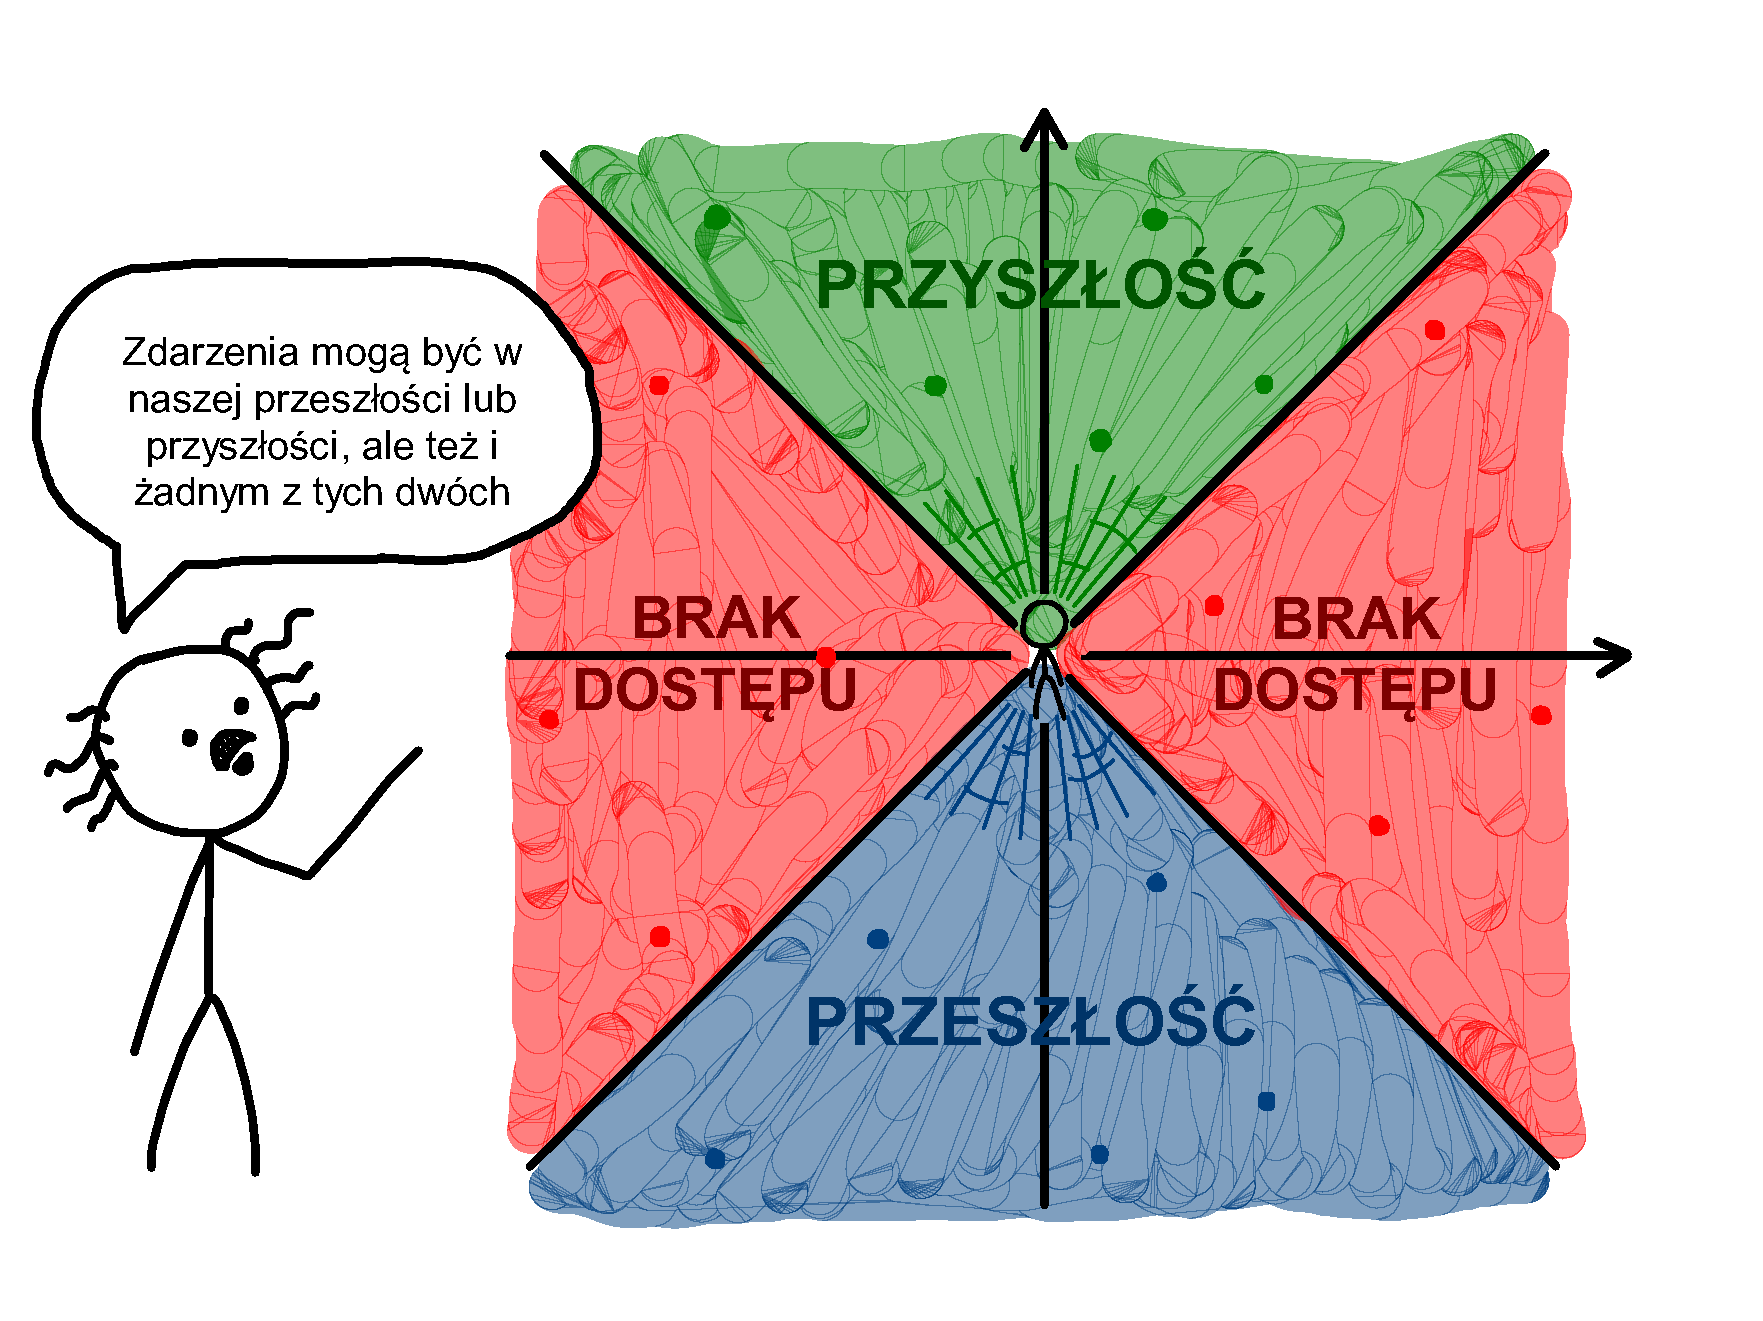
\includegraphics[width=1\linewidth]{pages/STA-page34}

Możemy wszystkie możliwe zdarzenia względem naszego ``tu i teraz'' umieścić na diagramie
czasoprzestrzennym i pokolorować według rodzaju interwału łączącego nas z tym zdarzeniem.

Zdarzenia, dla których interwał jest czasowy, uformują dwa stożki (tak zwane
stożki zerowe bo ich równanie to $ct^2 - x^2 = 0$).
Jeden zawierający naszą przyszłość, wszystkie zdarzenia, na które z
obecnego miejsca i czasu możemy mieć wpływ lub do nich dotrzeć.
Drugi zawierający naszą przeszłość. Wszystkie zdarzenia, które
mogą mieć teraz wpływać na nas.

Pozostaje jednak ogromny obszar zdarzeń, dla których interwał jest przestrzenny.
Są to wszystkie zdarzenia, które nie są ani w naszej przeszłości ani przyszłości.
Dla nas w tym momencie tak jakby nie istniały. Nie możemy ich zaobserwować
ani wejść w żadną inną interakcję.

Oczywiście nie pozostaną tam na zawsze. Jeśli poczekamy dostatecznie długo i
przesuniemy się w przód w czasie, to znajdą się one w stożku naszej przeszłości.
Zniknięcie Słońca w tej chwili będzie znajdować się poza naszym stożkiem zerowym,
ale za jakieś 8 min 19 s my przesuniemy się w czasoprzestrzeni tak, że to zdarzenie wpadnie
w obszar naszej przeszłości i poczujemy jego skutki.
\newpage

\subsection*{Pytania}
\begin{itemize}
  \item Dwa subluminalne ekspresy jadą naprzeciw ciebie z prędkościami $v_1 = 0.85c$
        i $v_2 = 0.90c$ względem torów. Z jaką prędkością zbliżają się do siebie według Alberta
        stojącego na stacji? Z jaką według maszynistów siedzących w pociągach?
  \item Beata wbiega do stodoły o długości własnej \SI{10}{ls} z prędkością $v = 0.866c$
        trzymając tyczkę o takiej samej długości własnej. Czy tyczka zmieści się
        w całości w stodole? Czy stodoła w całości obejmie tyczkę według Beaty?
  \item Stojące w szeregu Alberty wykonały nieskończenie szybką falę meksykańską
        podnosząc ręce jednocześnie. Z jaką szybkością i w jakim kierunku porusza
        się fala z punktu widzenia biegnącej wzdłuż nich Beaty?
        (Pamiętaj, że Beata umie biegać \textit{bardzo} szybko.)
\end{itemize}
\newpage

\noindent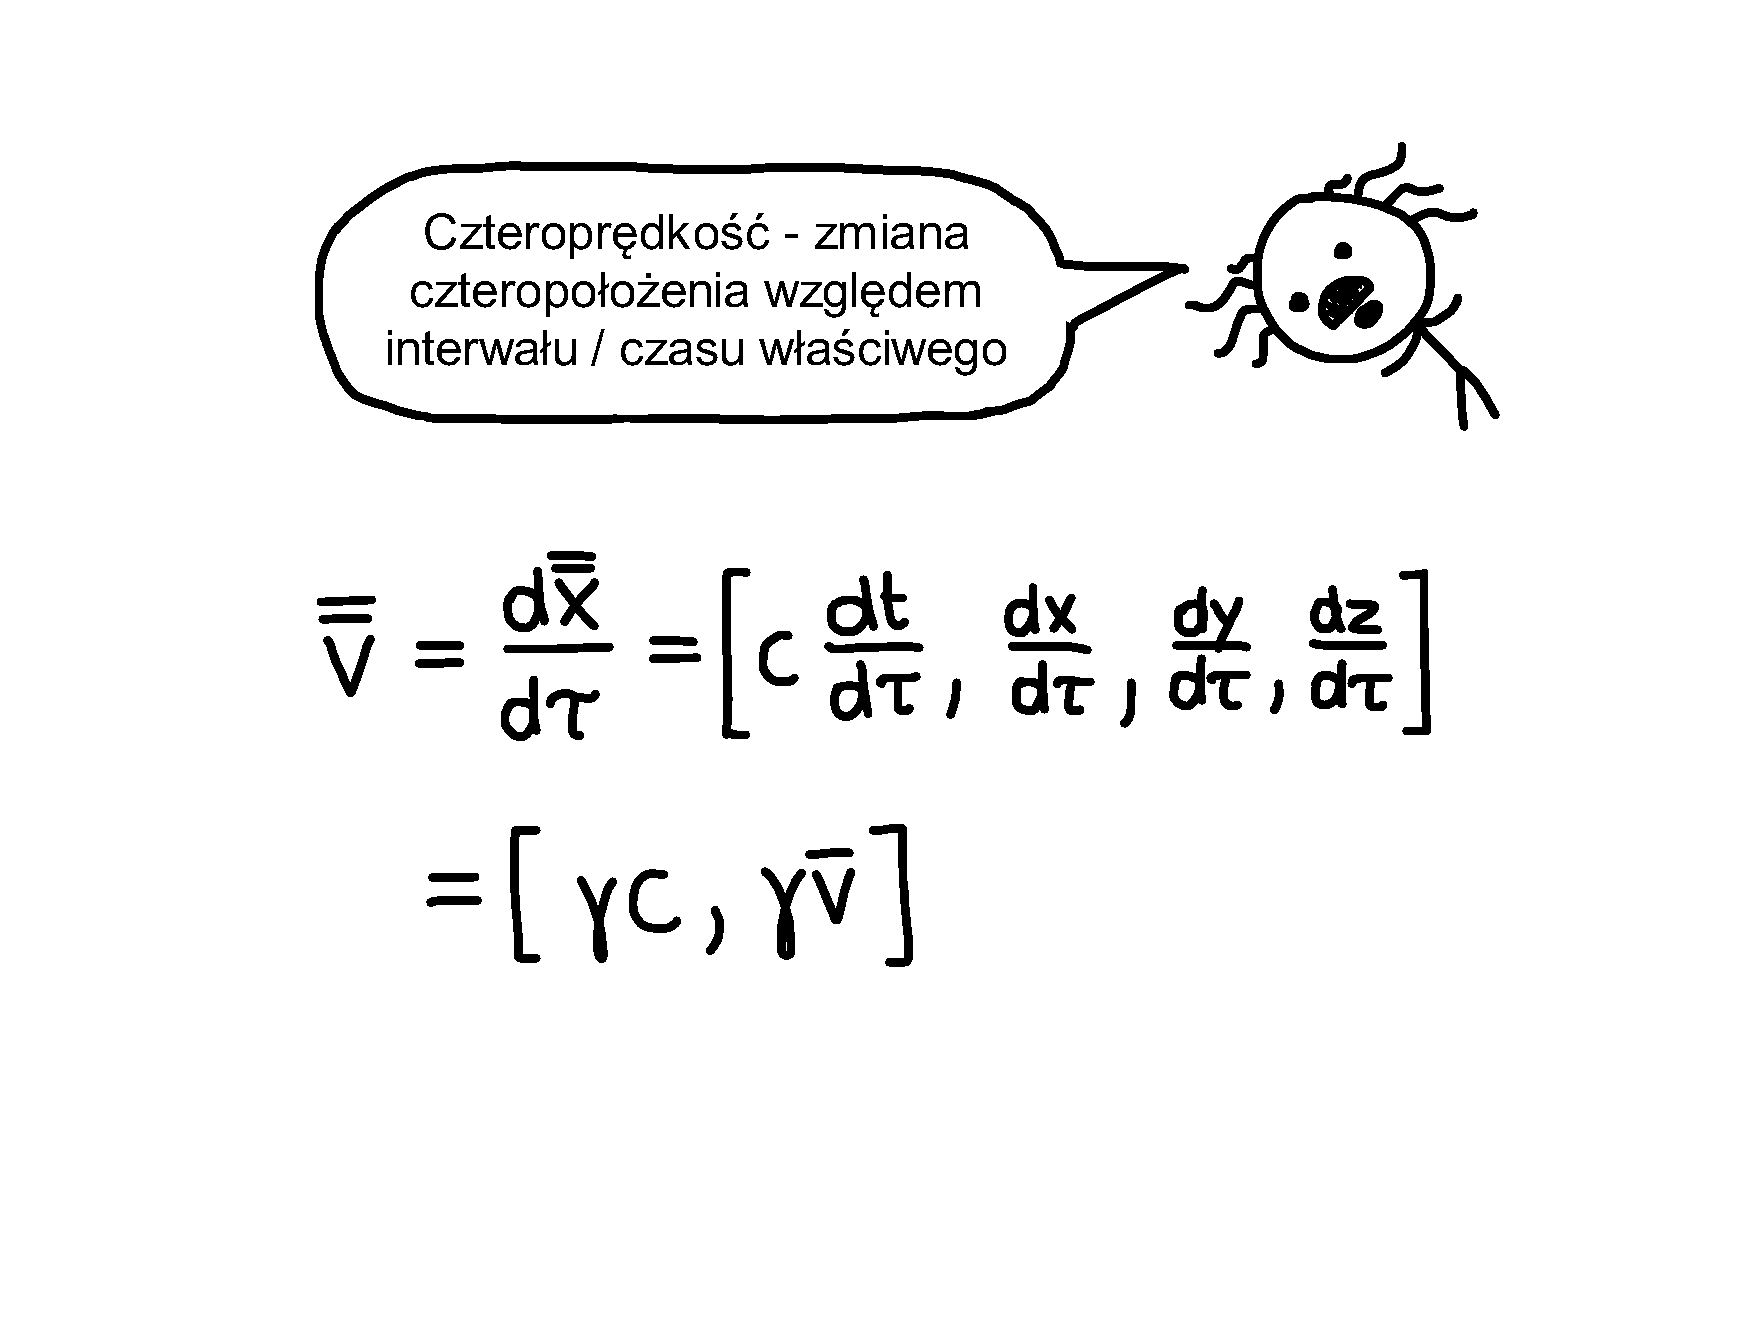
\includegraphics[width=1\linewidth]{pages/STA-page35}
Skoro wiemy już, że prędkości się nie dodają w sposób klasyczny, możemy
spróbować stworzyć jej relatywistyczny odpowiednik.
Podobnie jak z położenia zrobiliśmy czteropołożenie, którego ``długość'', czyli
interwał, jest niezmienny, to może analogicznie da się utworzyć podobną, czteroprędkość?

Jeśli jednak policzymy pochodną czteropołożenia po czasie to otrzymamy zwykłą
prędkość w kierunkach przestrzennych i $c$ w kierunku czasowym $[c, v_x, v_y, v_z]$.
Nie jest to zadowalające, bo taka prędkość nie transformuje się Lorentzowsko
jak ustaliliśmy wcześniej i jej ``długość'' nie jest niezmienna w różnych układach.
Wynika to z tego, że używany definicji prędkości $\derivative[x]{t}$, a przecież
$\diff t$ nie jest absolutne. Czynnik Lorentza z licznika kasuje nam się z czynnikiem
z mianownika pochodnej.

Absolutny jest jednak czas własny, czyli długość interwału, i to po nim możemy
policzyć pochodną. Czteroprędkość definiuje się zatem jako pochodna czteropołożenia
po czasie własnym
\[
  \fourvec{v} = \derivative[\fourvec{x}]{\tau} 
    = \left[c \derivative[t]{\tau}, \derivative[x]{\tau}, \derivative[y]{\tau}, \derivative[z]{\tau} \right].
\]
Robiąc parę przekształceń i podstawień otrzymujemy
\[ \fourvec{v}
  = \left[
    c\derivative[t]\tau,
    \derivative[x]t\derivative[t]{\tau},
    \derivative[y]t\derivative[t]{\tau},
    \derivative[z]t\derivative[t]{\tau}
    \right]
  = [\gamma c, \gamma v_x, \gamma v_y, \gamma v_z]. 
\]

Należy pamiętać jednak, że o ile czteropołożenie ma fizyczne znaczenie i
jest to obserwowane przez nas położenie i czas zdarzenia; to czteroprędkość
nie jest obserwowaną przez nas prędkością obiektu. Interpretacja czteroprędkości
to kierunek linii świata obiektu na diagramie czasoprzestrzennym. Stosunek
każdego komponentu czteropołożenia do interwału.
Jest to poniekąd wektor jednostkowy wskazujący kierunek ruchu na diagramie
czasoprzestrzennym. Dlaczego jednostkowy? Ponieważ jego ``długość'' to
\[
  (\gamma c)^2 - (\gamma v)^2 = (\gamma c)^2 - \left(\gamma c \frac{v}{c}\right)^2
   = (\gamma c)^2 \left(1 - \frac{v^2}{c^2}\right) = c^2.
\]

Niezależnie od prędkości i układu odniesienia, wszystko ma czteroprędkość
o wartości $c$.
\newpage

\noindent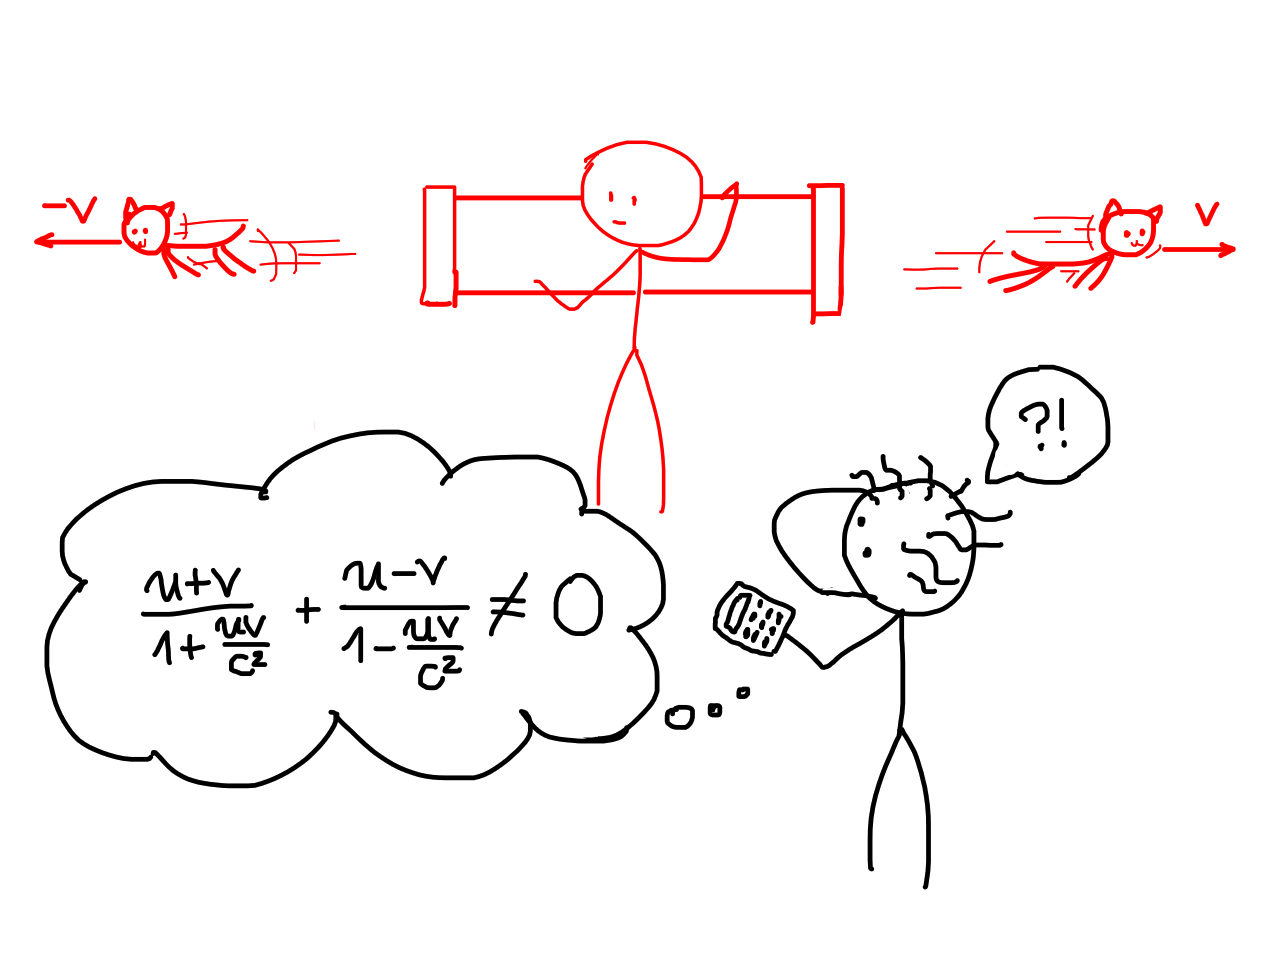
\includegraphics[width=1\linewidth]{pages/page-35-1.png}
Z dodawaniem prędkości jest jeszcze jeden, sporo poważniejszy, mankament.
Jeśli Beata wyrzuciłaby w przeciwnych kierunkach z tą samą prędkością dwa koty
o jednakowej masie, to ze względu na symetrię eksperymentu, powinna ona pozostać
w bezruchu. Przelatujący obok z prędkością $u$ Albert zmierzy jednak, że kot
wystrzelony w kierunku ruchu Beaty będzie wystrzelony wolniej, niż ten
wystrzelony w kierunku przeciwnym. Taka sytuacja łamie symetrię i z jego perspektywy
Beata powinna zmienić prędkość by pęd był zachowany, co jednak sie nie dzieje.

Szczególna teoria względności łamie zatem zasadę zachowania pędu, a przynajmniej
tą, sformułowaną przez Newtona. Newton jednak nie wiedział o elektrodynamice
i transformacji Lorentza i jego definicja pędu $p = mv$, również jest jedynie
przybliżeniem działającym przy małych prędkościach.

Jeśli zamiast prędkości, użyjemy współrzędnych przestrzennych czteroprędkości, to
okazuje się, że symetria znowu nam wraca. Więc czteroprędkość nie jest tak
całkowicie bezużyteczna.
\newpage

\noindent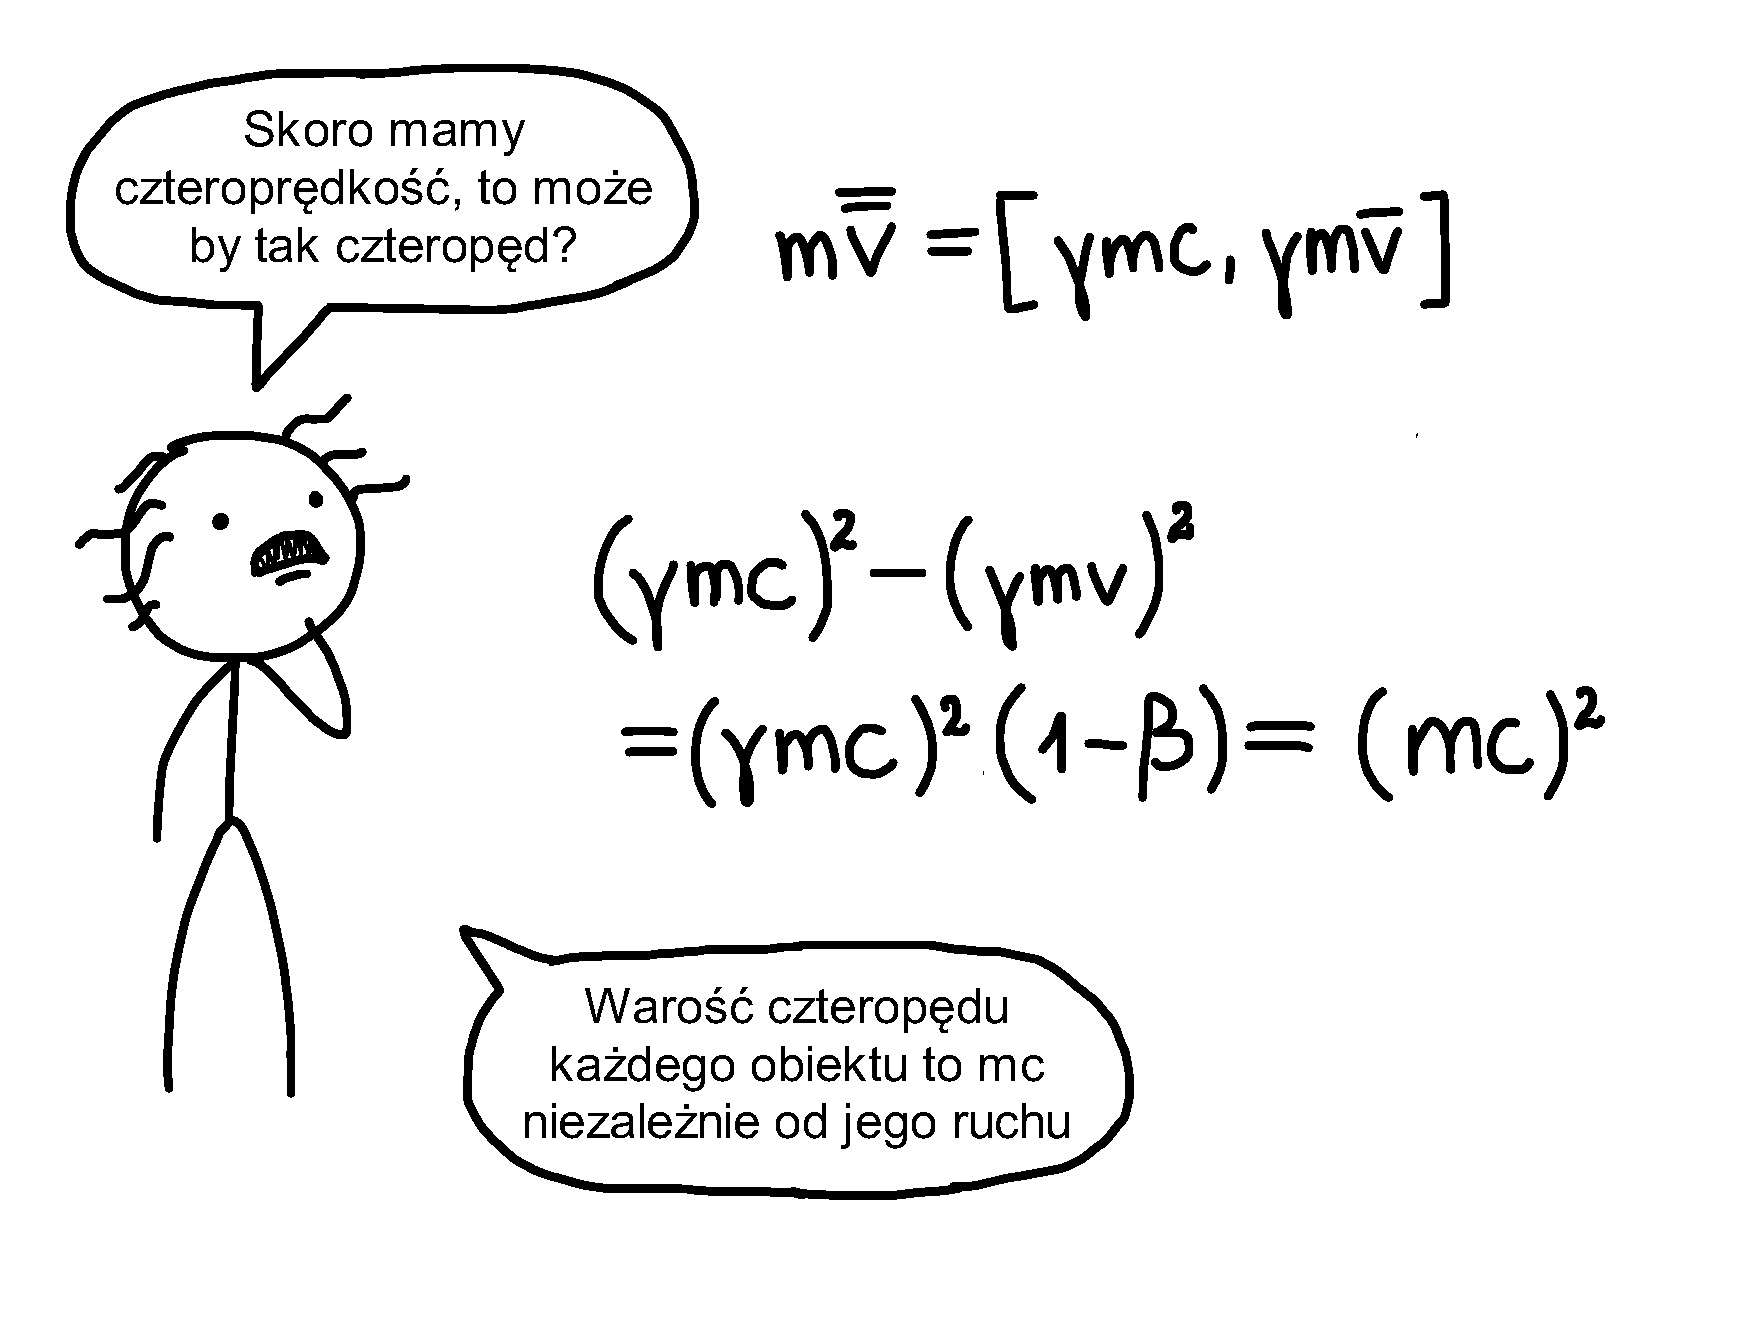
\includegraphics[width=1\linewidth]{pages/STA-page36}
Jeśli czteroprędkość zachowuje symetrię przestrzenną (i czasową też) to można
w takim razie użyć jej do zdefiniowania czteropędu
\[
  \fourvec{p} = m\fourvec{v} = [\gamma mc, \gamma m \vec v].
\]
Otrzymaliśmy nową definicję pędu z dodatkową, tajemniczą współrzędną w kierunku
czasowym.

Taki czteropęd transformuje się zgodnie z transformacją Lorentza przy zmianie
układu odniesienia i, podobnie do czteroprędkości, jego ``długość'' wynosi
\[
  (\gamma mc)^2 - (\gamma mv)^2 = (mc)^2.
\]

Pewnie już wam świta do czego to zmierza.
\newpage

\noindent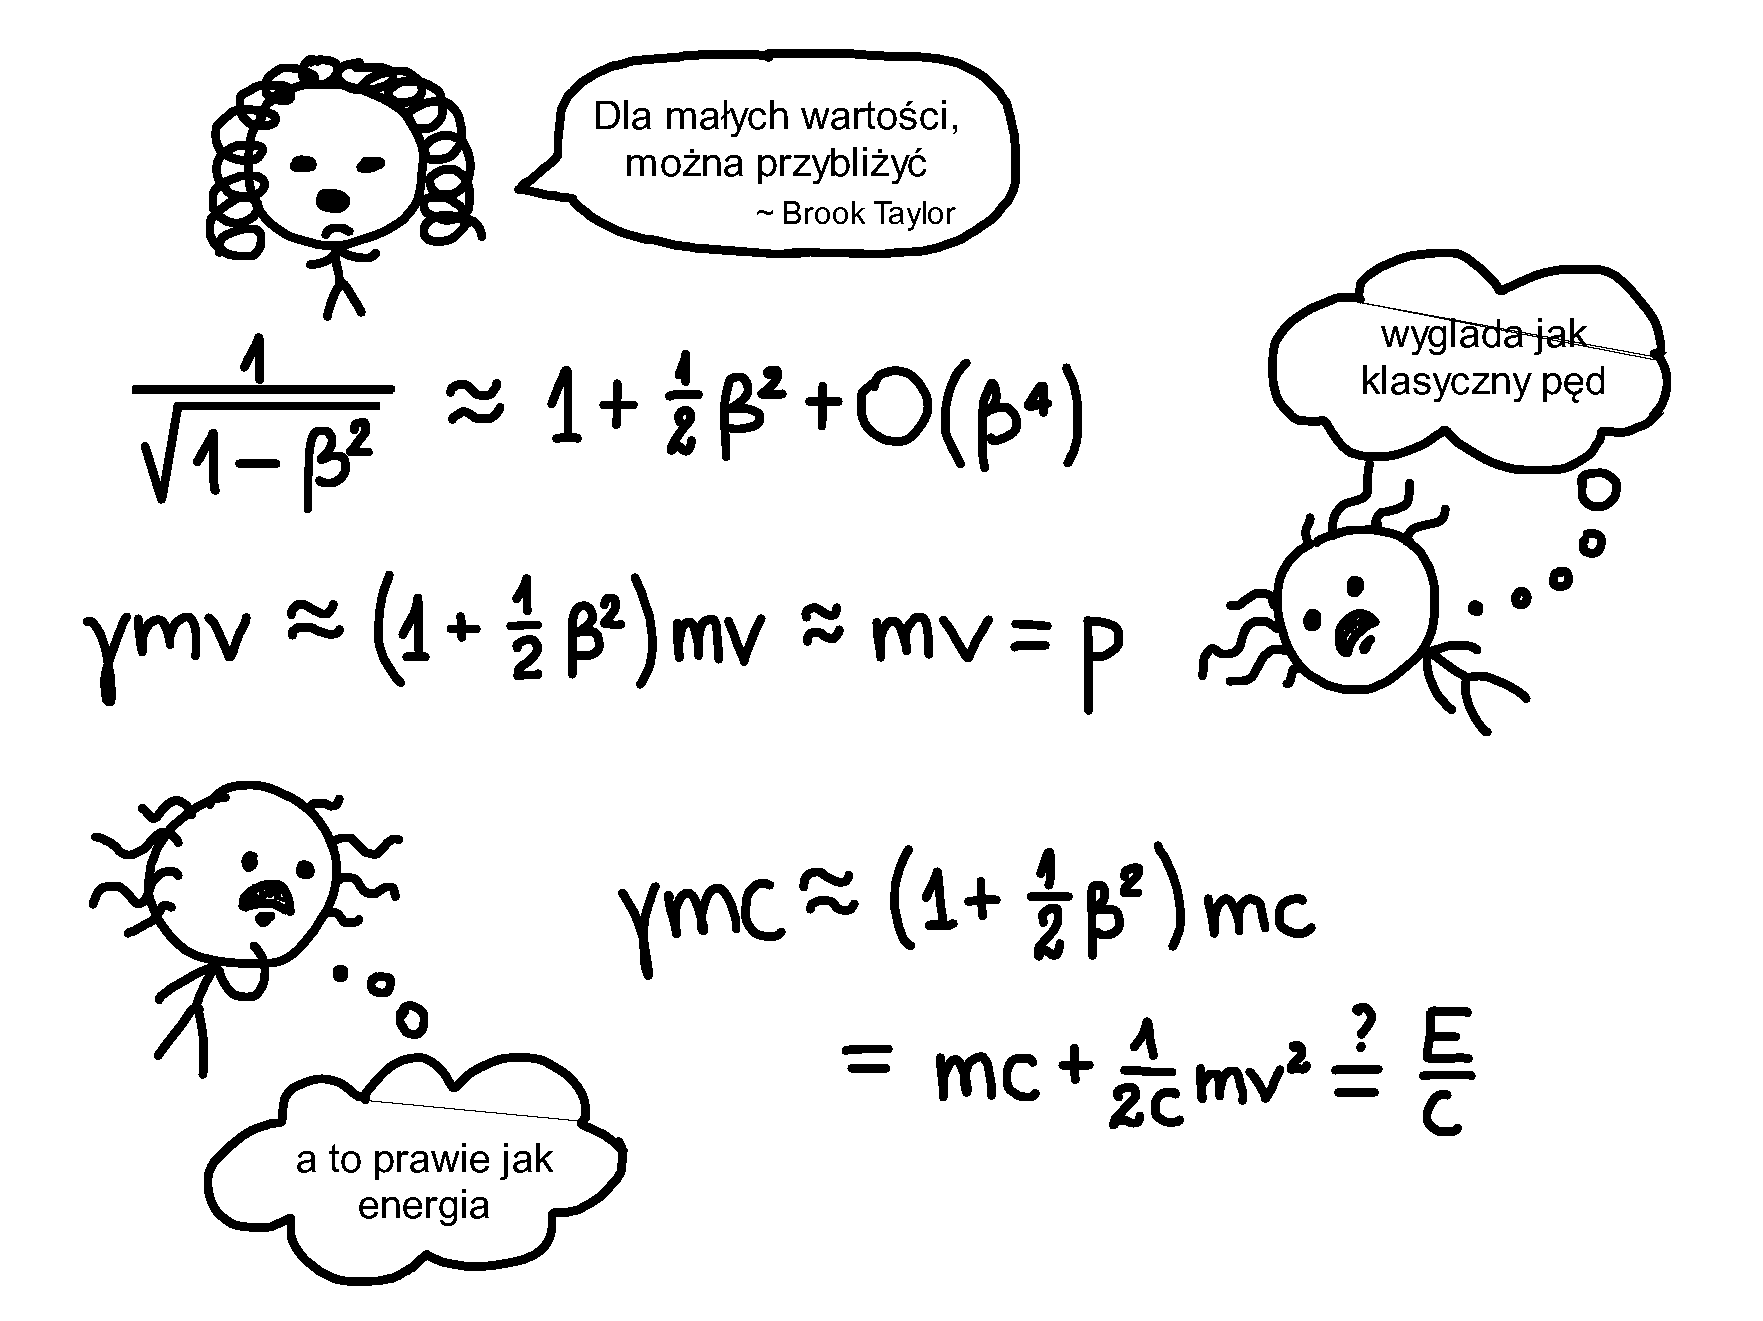
\includegraphics[width=1\linewidth]{pages/STA-page37}
Sprawdźmy do czego czteropęd się zbliża dla bardzo małych prędkości.
Z pomocą w przybliżeniu wartości $\gamma$ przychodzi nam szereg Taylora
\[
  \gamma = \frac{1}{\sqrt{1-\beta^2}} \approx 1 + \frac{1}{2}\beta^2 + O(\beta^4).
\]

Podstawiając do części przestrzennej czteropędu otrzymujemy
\[
  \gamma mv \approx (1 + \frac{1}{2}\beta^2)mv \approx mv = p.
\]
Część przestrzenna to nic innego jak zwykły pęd.
A co ze współrzędną czasową?
\[
  \gamma mc \approx (1 + \frac{1}{2}\beta^2)mc = mc + \frac{1}{2c}mv^2 \stackrel?= \frac{E}{c}.
\]
To przypomina energię kinetyczną z dodatkowym wyrazem $mc^2$.
Jeśli całe to wyrażenie potraktujemy jako energię, to by znaczyło, że
nieruchome obiekty też posiadają energię ``kinetyczną'' wynikającą z przemieszczania
się z przeszłości w przyszłość. Nazywanie jednak energii nie ruszania się kinetyczną
jest trochę głupie, więc nazwano to \textit{energią spoczynkową}.

\newpage

\noindent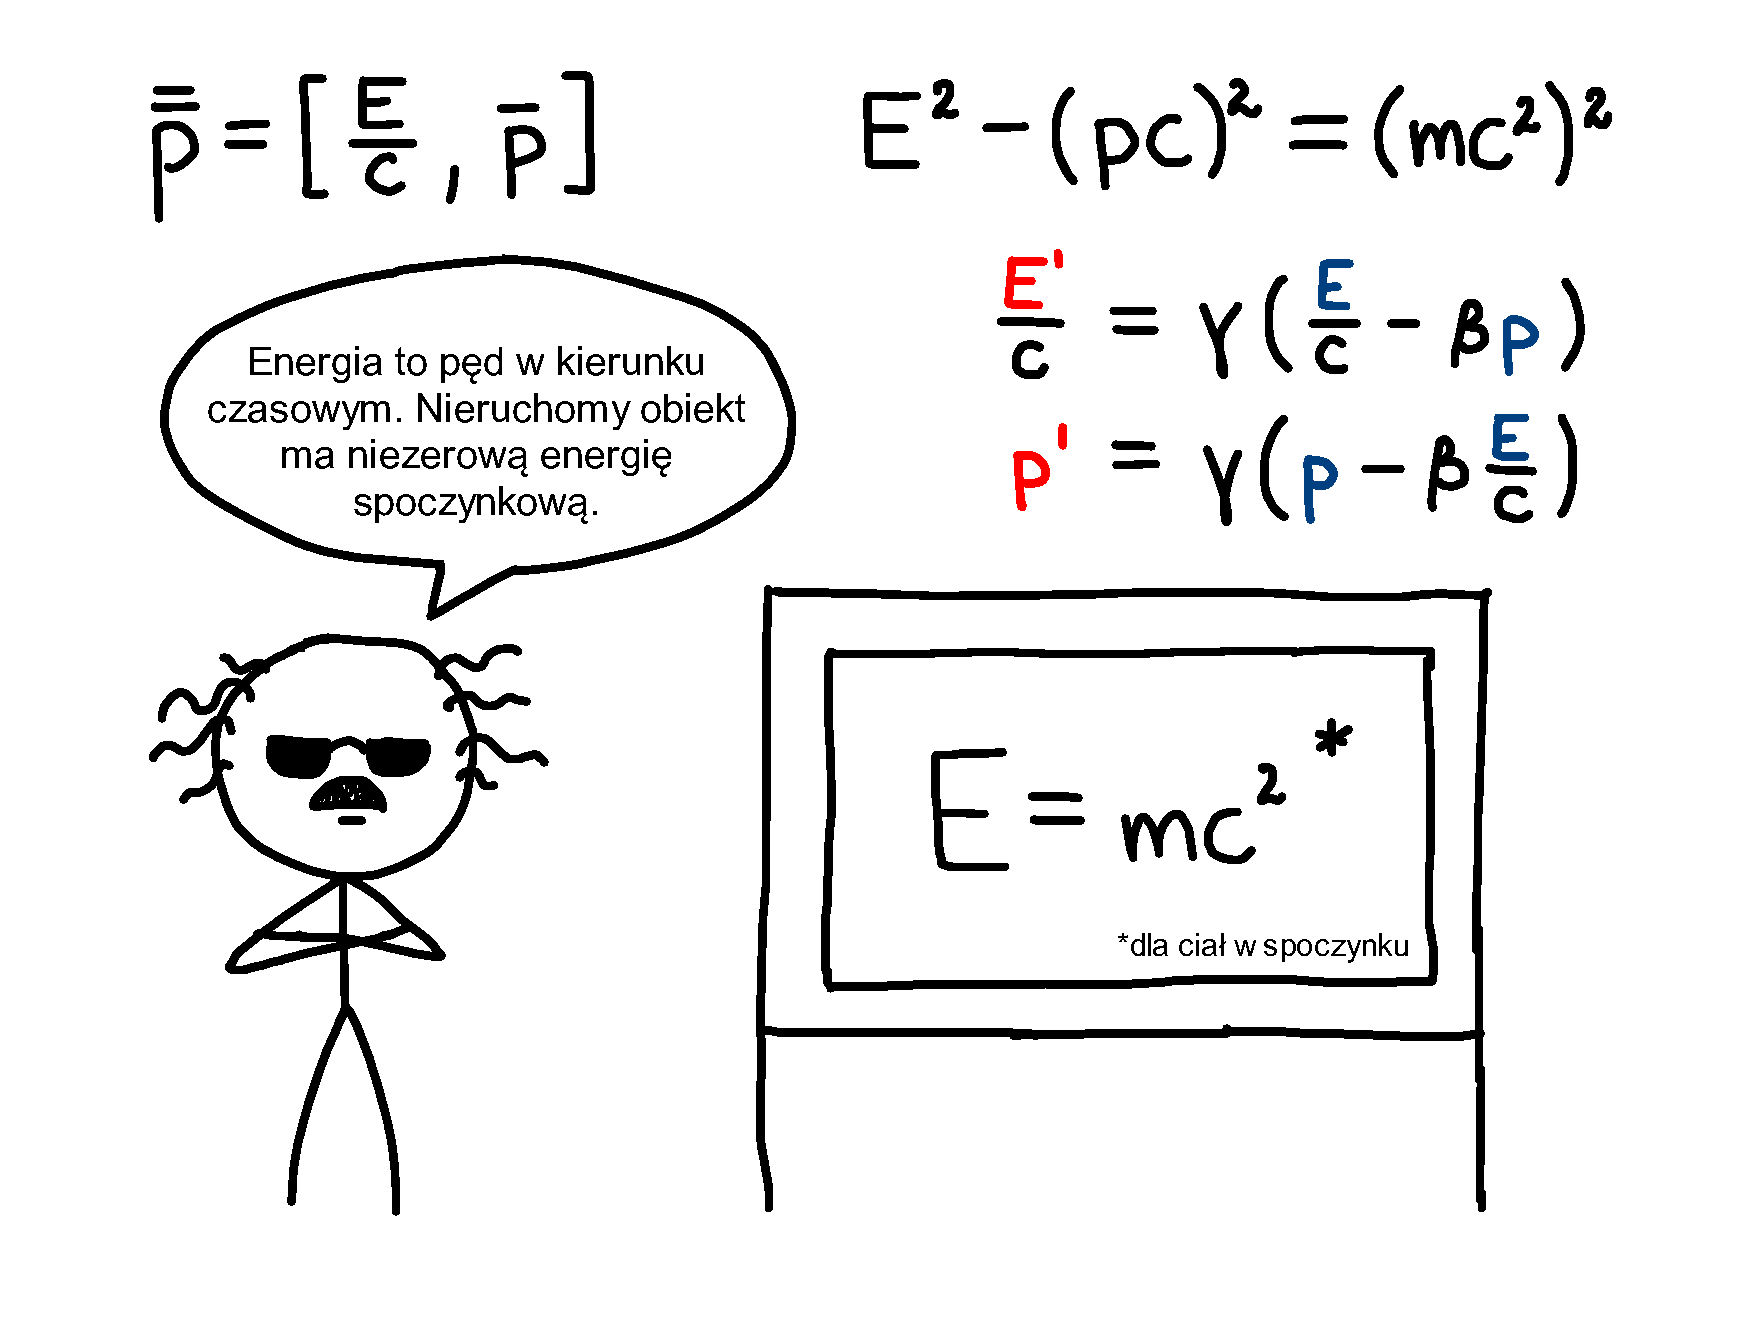
\includegraphics[width=1\linewidth]{pages/STA-page38}
Cały wektor czteropędu można zatem przestawić przy pomocy energii i pędu.
Mało kreatywni fizycy nazwali go wektorem energii-pędu.
\[\fourvec p = \left[\frac{E}{c}, \vec p\right]\]

Jego czterowymiarowa ``długość'' wynosi, jak już ustaliliśmy poprzednio,
\[ E^2 - (pc)^2 = (mc^2)^2, \]
gdzie $E = \gamma mc$ oraz $p = \gamma mv$ to relatywistyczna energia i pęd.

Ten czterowektor, tak jak wszystkie inne, przekształca sie transformacją Lorentza
przy zmianie układu odniesienia
\[
  \begin{eqsystem}
    \frac{\mred{E'}}{c} = \gamma \left(\frac{\mblue{E}}{c} - \beta \mblue{p}\right) \\
    \mred{p'} = \gamma \left(\mblue{p} - \beta \frac{\mblue E}{c}\right)
  \end{eqsystem}.
\]

Te równania są jednymi z najważniejszych w fizyce cząstek i nuklearnej.
Pozwalają na policzenie energii oraz pędu cząstek przy ekstremalnych energiach,
które towarzyszą rozpadom jądrowym lub reakcjom w zderzaczach hadronów.
\newpage

\noindent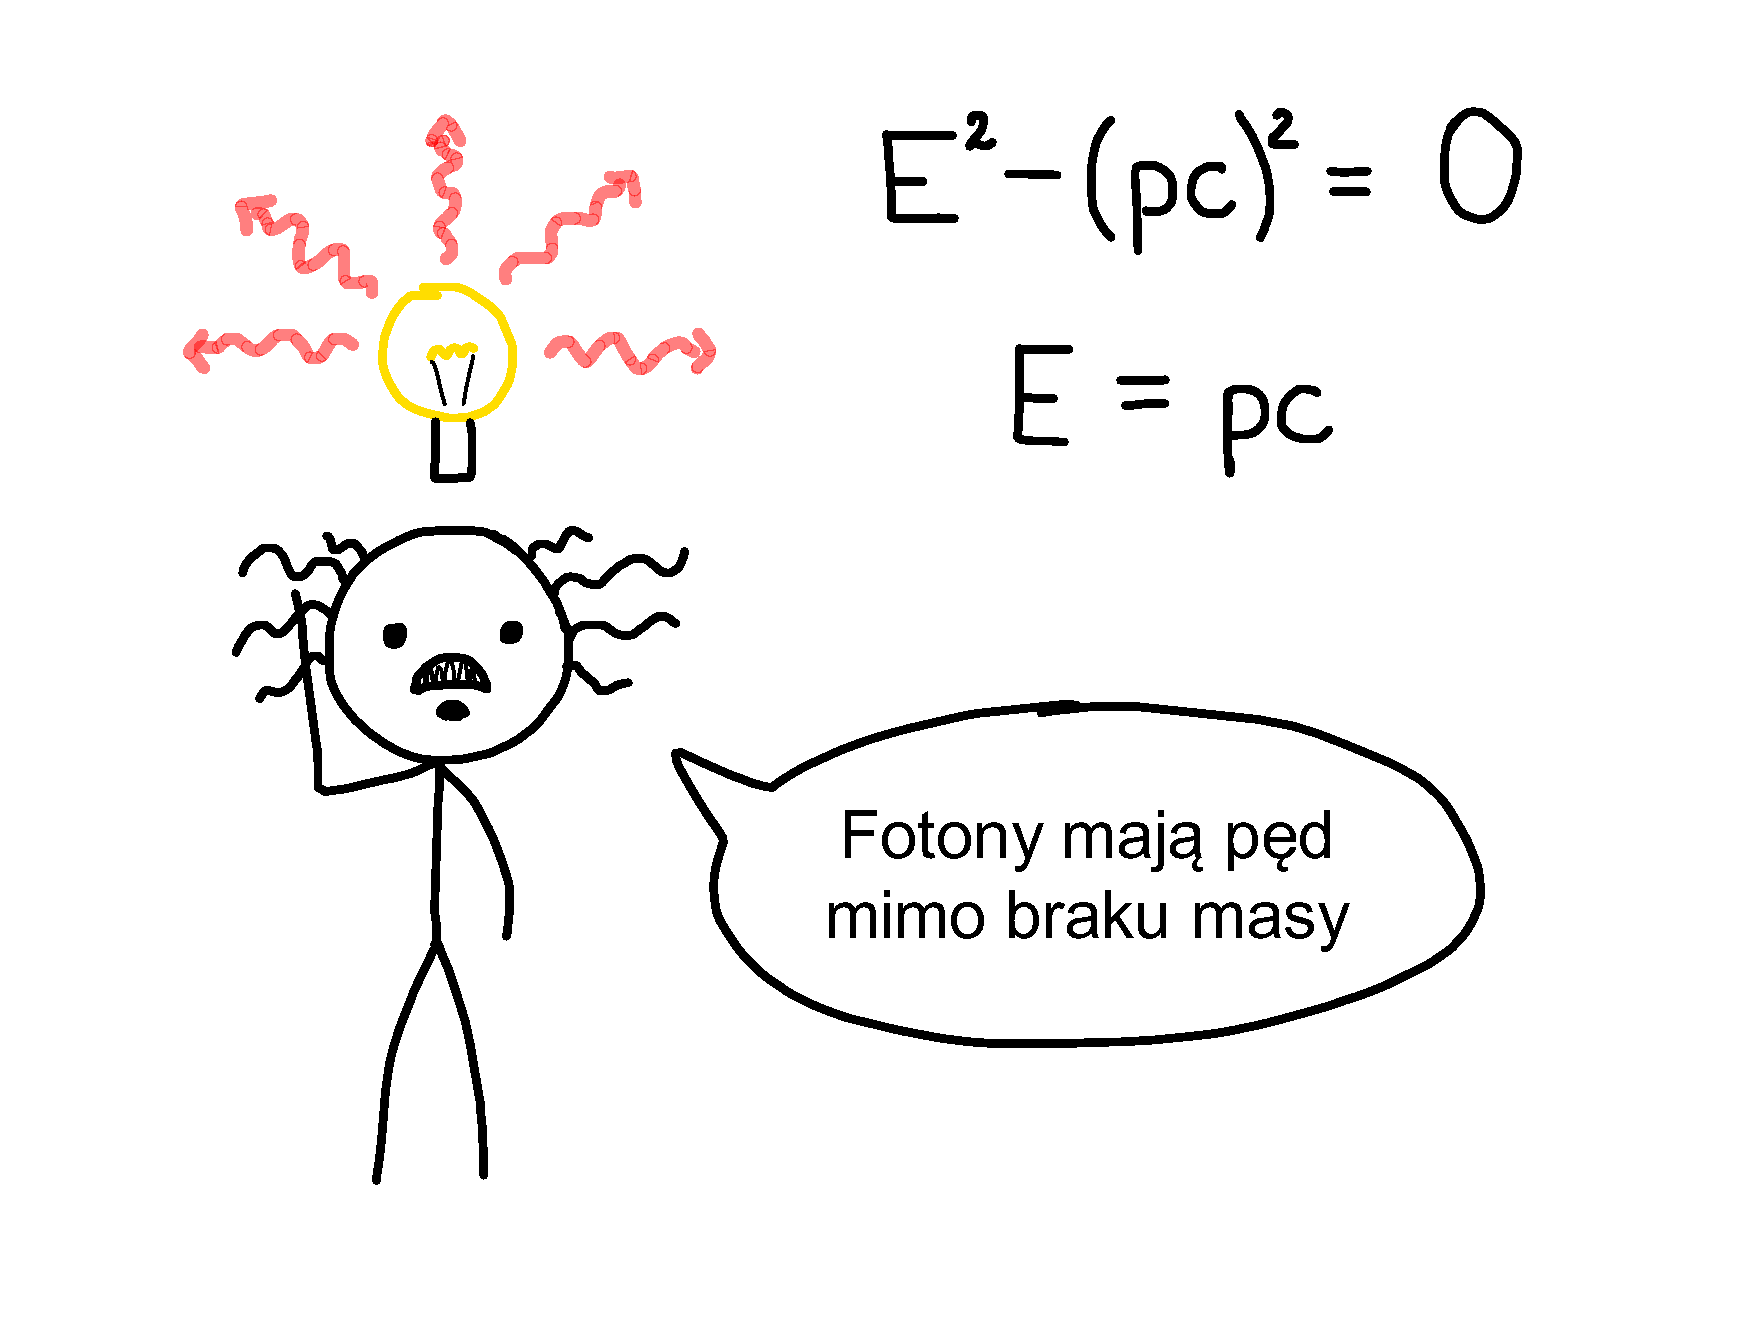
\includegraphics[width=1\linewidth]{pages/STA-page39}
Z analizy relatywistycznej energii i pędu można wyciągnąć jeszcze jeden ciekawy
wniosek. Jeśli coś nie posiada masy a posiada energię, jak na przykład fala
elektromagnetyczna, to koniecznie posiada też pęd.
\begin{gather*}
  E^2 - (pc)^2 = 0, \\
  E = pc.
\end{gather*}
Coś co w klasycznej mechanice byłoby nie do pomyślenia.

Co więcej, żeby ten warunek był spełniony to wszystkie bezmasowe obiekty muszą
poruszać się z prędkością światła i wszystko co porusza się z prędkością światła
musi nie mieć masy. W przeciwnym razie miałyby zerową energię i by nie istniały
lub miałyby nieskończoną energię i też by nie istniały.
\newpage

\section*{Pytania}
\begin{itemize}
\item Dwie wiązki protonów rozpędzone do całkowitej energii \SI{0.59}{TeV}
      zderzają się czołowo całkowicie nieelastycznie. Ile energii zostanie
      wyzwolone w każdym zderzeniu?
\item Jedna wiązka protonów rozpędzona do energii \SI{1.18}{TeV} zderza się
      nieelastycznie z nieruchomymi atomami złota. Ile energii zostanie teraz
      wyzwolone w zderzeniu?
\item Irradiancja, czyli moc promieniowania na jednostkę powierzchni, światła
      słonecznego padającego prostopadle na lustro wynosi
      \SI{0.93}{\watt\per\meter\squared}. Jakie ciśnienie wywiera odbijane
      światło na lustro?
\end{itemize}
\newpage

\section{Dodatki}
\section*{Transformacje współrzędnych}

Najprostszym rodzajem transformacji współrzędnych jest \textbf{przesunięcie}
punktu o stałą wartość np. o wektor $(t_x, t_y)$. Nowe współrzędne $(x', y')$
można wtedy wyrazić przy pomocy starych $(x, y)$ jako:
\[
  \begin{eqsystem}
    x' = x + t_x \\
    y' = y + t_y
  \end{eqsystem}.
\]
Przekształcając to równanie możemy łatwo wyznaczyć jak taką transformację
odkręcić
\[
  \begin{eqsystem}
    x = x' - t_x \\
    y = y' - t_y
  \end{eqsystem}.
\]

Inną prostą transformacją jest \textbf{rozciągnięcie} podczas którego każda
ze współrzędnych skaluje przez pewien czynnik np. $s_x, s_y$.
Nowe współrzędne można wyrazić jako:
\[
  \begin{eqsystem}
    x' = s_x \cdot x \\
    y' = s_y \cdot y
  \end{eqsystem}.
\]

Do nieco bardziej złożonych transformacji należy \textbf{obrót} i
\textbf{pochylenie} (ścinanie). W ich przypadku współrzędne $x$ i $y$ nie
przekształcają się niezależnie od siebie.
Obrót punktu wokół środka układu współrzędnych o kąt $\theta$ przeciwnie do ruchu
wskazówek zegara będzie dany układem równań:
\[
  \begin{eqsystem}
    x' = x \cos \theta - y \sin \theta \\
    y' = x \sin \theta + y \cos \theta
  \end{eqsystem}.
\]

W przypadku pochylenia osobno traktujemy pochylenie wzdłuż osi $x$ oraz $y$.
Pochylenie o kąt $\phi$ równoległe do osi $x$ wyraża układ:
\[
  \begin{eqsystem}
    x' = x + y \tan\phi \\
    y' = y
  \end{eqsystem}.
\]
Analogicznie możemy pochylić współrzędne równolegle do osi $y$:
\[
  \begin{eqsystem}
    x' = x \\
    y' = x \tan\phi + y
  \end{eqsystem}.
\]
Nie należy mylić pochylenia z obrotem. Kwadrat po obróceniu nadal jest kwadratem,
zaś po pochyleniu będzie równoległobokiem.

Przepisywanie układów równań nie należy do najprzyjemniejszych czynności, a
matematycy i fizycy lubią iść na skróty. Tak też się stało w przypadku transformacji
współrzędnych. Zamiast obliczać przekształcenie dla $x$ i $y$ osobno, można obie
współrzędne wrzucić w jeden wektor. Transformacja obywa się wtedy poprzez
iloczyn \textit{macierzy transformacji} oraz tego wektora.
Przykładowo, pochylenie możemy teraz zapisać jako:
\[
  \begin{bmatrix}x' \\ y'\end{bmatrix} =
  \begin{bmatrix}1 & \tan\phi \\ 0 & 1\end{bmatrix}
  \begin{bmatrix}x \\ y\end{bmatrix} =
  \begin{bmatrix}x + y\tan\phi \\ y\end{bmatrix}
\]

Nic nas nie ogranicza, aby nakładać transformacje jedna po drugiej. Możemy
wykonać kilka przekształceń na raz ustawiając je od prawej do lewej.
\[
  \begin{bmatrix}
    x' \\ y'
  \end{bmatrix} =
  \underbrace{
    \begin{bmatrix}
      \cos \theta & -\sin \theta \\
      \sin \theta & \cos \theta
    \end{bmatrix}
  }_\text{obrót}
  \underbrace{
    \begin{bmatrix}
      s_x & 0   \\
      0   & s_y
    \end{bmatrix}
  }_\text{rozciągnięcie}
  \begin{bmatrix}
    x \\ y
  \end{bmatrix}.
\]
W pierwszej kolejności na współrzędne działa rozciągnięcie a potem obrót.
Wektor najpierw mnożymy przez macierz najbardziej po prawej i wynik kolejno
redukujemy od prawej do lewej.

Ponieważ mnożenie macierzy kwadratowych jest łączne, możemy je ze sobą grupować.
Należy jednak pamiętać, że kolejność wykonania operacji jest istotna,
przeskalowanie a potem obrót to nie to samo co obrót a potem przeskalowanie
\[
  % \begin{split}
  \underbrace{
    \begin{bmatrix}
      1 & 0 \\ \tan\phi & 1
    \end{bmatrix}
  }_\text{pochylenie}
  \bigg(
  \underbrace{
    \begin{bmatrix}
      s_x & 0 \\ 0 & s_y
    \end{bmatrix}
  }_\text{rozciągnięcie}
  \begin{bmatrix}
    x \\ y
  \end{bmatrix}
  \bigg) =
  \bigg(
  \underbrace{
    \begin{bmatrix}
      1 & 0 \\ \tan\phi & 1
    \end{bmatrix}
  }_\text{pochylenie}
  \underbrace{
    \begin{bmatrix}
      s_x & 0 \\ 0 & s_y
    \end{bmatrix}
  }_\text{rozciągnięcie}
  \bigg)
  \begin{bmatrix}
    x \\ y
  \end{bmatrix} =
  \mkern-15mu
  \underbrace{
    \begin{bmatrix}
      s_x & 0 \\ s_x \tan\phi & s_y
    \end{bmatrix}
  }_\text{rozciągnięcie i pochylenie}
  \mkern-15mu
  \begin{bmatrix}
    x \\ y
  \end{bmatrix}
  % \end{split}
\]

W ogólności, dowolna transformacja liniowa sprowadza się do macierzy:
\[
  \begin{bmatrix}
    A & B \\
    C & D
  \end{bmatrix}
  \begin{bmatrix}
    x \\ y
  \end{bmatrix} =
  \begin{bmatrix}
    Ax + By \\
    Cx + Dy
  \end{bmatrix}.
\]

Mogłeś zauważyć już pewien mankament. Nie da się w ten sposób zapisać przesunięcia!
To dlatego, że przesunięcie nie jest legalną transformacją liniową. Matematycznym
warunkiem transformacji liniowej jest aby punkt $(0, 0)$ przekształcała
w samego siebie, czego przesuniecie nie spełnia.
Możemy w takiej sytuacji zrobić wyjątek i samodzielnie przesunąć punkt w odpowiednim
momencie dodając współrzędne jak tutaj:
\[
  \begin{bmatrix}x' \\ y'\end{bmatrix} =
  \underbrace{\begin{bmatrix}
      \cos \theta  & \sin \theta \\
      -\sin \theta & \cos \theta
    \end{bmatrix}}_{\text{obrót}}
  \bigg(
  \begin{bmatrix}x \\ y\end{bmatrix} + \mkern-20mu
  \underbrace{\begin{bmatrix}t_x \\ t_y\end{bmatrix}}_{\text{przesunięcie}}
  \mkern-20mu
  \bigg),
\]
ale psujemy wtedy piękno i prostotę mnożenia.

\newpage
\section*{Dlaczego transformacja Lorentza musi być liniowa?}
W jaki sposób z przesłanki, że transformacja Lorentza musi odbywać się tak samo w każdym miejscu
i czasie we wszechświecie wynika, że jest liniowa?
Nie jest to takie oczywiste na pierwszy rzut oka ale staje się jasne, gdy spojrzy się
na kontrprzykład.
Załóżmy, że transformacja \textbf{nie jest} liniowa i wynosi na przykład
\[x' = Ax + Bt^2.\]
Licząc z tego równania przyrosty (różniczki) otrzymujemy
\[\Delta x' = A \Delta x + 2Bt \Delta t.\]
Wynika z tego, że w inercjalnym układzie $(t', x')$ kij o długość $\Delta x'$ robiłby się
coraz dłuższy wraz z upływem czasu.
Każde użycie funkcji innej niż liniowa będzie skutkować zmieniającymi się długościami
obiektów w układach inercjalnych, co jest niedopuszczalne i łamie zasadę, że prawa fizyki
we wszystkich układach inercjalnych muszą być takie same.
Jedynie funkcja liniowa daje nam pochodną, która jest stałą.

Dla porównania, transformacja liniowa daje
\[x' = Ax + Bt\]
\[\Delta x' = A\Delta x + B\Delta t.\]
Długości zmienią się przy przejściu między układami, ale w obrębie jednego układu
inercjalnego będą niezmienne.

\end{document}
